\documentclass[twoside,makeidx]{book}
% set paper size and margins; needs to be adapted for A5 ideally, we
% should have a document class for conference handbooks where A5
% vs. letter-halved is a class option
\usepackage[
  paperheight=8.5in, 
  paperwidth=5.5in, 
  inner=.75in,
  outer=.5in,
  bottom=.75in,
  top=.75in,
  twoside]{geometry}
\usepackage[T1]{fontenc}
\usepackage[utf8]{inputenc}
\usepackage{textcomp}
\usepackage{graphicx}
\usepackage{color}
\definecolor{mygray}{gray}{0.75}
\usepackage{colortbl}
\usepackage{fancyhdr}
\usepackage[Bjornstrup]{fncychap}
\usepackage{longtable}
\usepackage{tabularx}
\usepackage{lscape}
\usepackage{array}
\usepackage{calc}
\usepackage{csquotes}
\usepackage[american]{babel}
\usepackage{multicol}
\usepackage{multirow}
\usepackage{times}
\usepackage{helvet}
\usepackage[maxnames=25,minnames=3,babel=hyphen]{biblatex}
\usepackage{bibentry}
\usepackage{setspace}
\usepackage{ifthen}
\usepackage{pstricks}
\usepackage{rotating}
\usepackage{makeidx}

%\providecommand{\BIBand}{and}

\newcommand{\leftheader}{}  
\newcommand{\rightheader}{} 
\pagestyle{fancy}
  % header spec
  %\renewcommand{\headrule}{{\color[rgb]{0.696,0,0}% 
  \renewcommand{\headrule}{{\color[rgb]{0.132,0.125,.46}% 
    \hrule height 2pt width \headwidth}
    \vspace{1pt}%
    {\color{mygray}%
    \hrule height 1pt width \headwidth
  \vspace{-4pt}}}

  \fancyhf{}				       % clear header contents
  %\fancyhead[LE]{\textit{\nouppercase{\leftmark}}}
  %\fancyhead[RO]{\textit{\nouppercase{\rightmark}}} % define header contents
  \fancyhead[LE]{\textit{\nouppercase{\leftheader}}}
  \fancyhead[RO]{\textit{\nouppercase{\rightheader}}} % define header contents

  % footer spec
  \renewcommand{\footrule}{\hrule width \headwidth height 1mm\vskip\footruleskip}
  \renewcommand{\footruleskip}{0.5\normalbaselineskip}
  \fancyfoot[C]{\thepage}			 %define footer conten

%  \rfoot{\setlength{\unitlength}{1mm} % logo in right part of footer
%  \begin{picture}(0,0)
    %\put(-13,-10){\includegraphics[scale=0.3]{images/conf.jpg}}%
%    \put(-10,-5){\includegraphics[scale=0.2]{images/conf.jpg}}%
%  \end{picture}}

\makeatletter
\renewcommand\chapter{\if@openright\cleardoublepage\else\clearpage\fi %let headers/footers show on pages that start a chapter
                    \global\@topnum\z@
                    \@afterindentfalse
                    \secdef\@chapter\@schapter}

\renewcommand{\chaptermark}[1]{\markboth{#1}{}} % show chapter in header w/o numbering
\renewcommand{\sectionmark}[1]{\markright{#1}{}} % show section in headers w/o numbering

% redefine sections to have a horizontal rule and no numbering
\def\section{\@ifstar\unnumberedsection\numberedsection}
\def\numberedsection{\@ifnextchar[%]
  \numberedsectionwithtwoarguments\numberedsectionwithoneargument}
\def\unnumberedsection{\@ifnextchar[%]
  \unnumberedsectionwithtwoarguments\unnumberedsectionwithoneargument}
\def\numberedsectionwithoneargument#1{\numberedsectionwithtwoarguments[#1]{#1}}
\def\unnumberedsectionwithoneargument#1{\unnumberedsectionwithtwoarguments[#1]{#1}}
\def\numberedsectionwithtwoarguments[#1]#2{
  \ifhmode\par\fi
  \removelastskip
  \vskip 3ex\goodbreak
  \refstepcounter{section}%			   % increment counter
  \begingroup
  \noindent\begin{minipage}{\columnwidth}
  \leavevmode\Large\bfseries\raggedright
%  \thesection\  % leave out numbering
  #2 \par\nobreak
  \vskip -.5em
  \noindent\hrulefill\nobreak
  \end{minipage}
  \endgroup
  \vskip 1ex\nobreak
  \markright{#1}{} % add mark to right (secondary) header
  \addcontentsline{toc}{section}{%
%    \protect\numberline{\thesection}% % leave out number
    #1}%
  }
\def\unnumberedsectionwithtwoarguments[#1]#2{
  \ifhmode\par\fi
  \removelastskip
  \vskip 3ex\goodbreak
  \begingroup
  \noindent\begin{minipage}{\columnwidth}
  \leavevmode\Large\bfseries\raggedright
  #2\par\nobreak
  \vskip -.5em
  \noindent\hrulefill\nobreak
  \end{minipage}
  \endgroup
  \vskip 1ex\nobreak
  \markright{#1}{} % add mark to right (secondary) header
  }

% redefine subsections to have a horizontal rule and no numbering
\def\subsection{\@ifstar\unnumberedsubsection\numberedsubsection}
\def\numberedsubsection{\@ifnextchar[%]
  \numberedsubsectionwithtwoarguments\numberedsubsectionwithoneargument}
\def\unnumberedsubsection{\@ifnextchar[%]
  \unnumberedsubsectionwithtwoarguments\unnumberedsubsectionwithoneargument}
\def\numberedsubsectionwithoneargument#1{\numberedsubsectionwithtwoarguments[#1]{#1}}
\def\unnumberedsubsectionwithoneargument#1{\unnumberedsubsectionwithtwoarguments[#1]{#1}}
\def\numberedsubsectionwithtwoarguments[#1]#2{
  \ifhmode\par\fi
  \removelastskip
  \vskip 3ex\goodbreak
  \refstepcounter{subsection}%			   % increment counter
  \begingroup
  \noindent
  \leavevmode\normalsize\bfseries\raggedright
%  \thesubsection\  % leave out numbering
  #2 \par\nobreak
  \endgroup
  \vskip 1ex\nobreak
  \addcontentsline{toc}{subsection}{%
%    \protect\numberline{\thesubsection}% % leave out number
    #1}%
  }
\def\unnumberedsubsectionwithtwoarguments[#1]#2{
  \ifhmode\par\fi
  \removelastskip
  \vskip 3ex\goodbreak
  \begingroup
  \noindent
  \leavevmode\normalsize\bfseries\raggedright
  #2\par\nobreak
  \endgroup
  \vskip 1ex\nobreak
  }

\makeatother

% Clears to an even-numbered page
\def\clearevenpage{
     \clearpage 
     \ifodd\value{page} \hbox{}\newpage\fi
}

% Clears to the back-cover (for logos)
\def\cleartobackcover{
     \clearpage 
     \ifodd\value{page}\pagestyle{empty}\clearevenpage \else\hbox{}\cleardoublepage\pagestyle{empty}\clearevenpage\fi
}

%\renewcommand{\cleardoublepage}{\clearpage}

% Min: index
\makeindex

%\raggedbottom
%\setlength{\parindent}{0pt}
% Unicode issues
% \DeclareUnicodeCharacter{fi}{fi}

% Min: correct column widths
\newlength{\mycolumnwidth}
\setlength{\mycolumnwidth}{\columnwidth}
\addtolength{\mycolumnwidth}{-2ex}

\renewcommand{\textfraction}{.2}
\renewcommand{\bottomfraction}{.8}

\newenvironment{bio}{%
  \begin{figure}[b]
  \centerline{\rule{.5\linewidth}{.5pt}}\vspace{2ex}}%
{\end{figure}}

\setlength{\parindent}{1em}

\fancypagestyle{emptyheader}
{
  \fancyhf{}
  \fancyfoot[C]{\thepage}
}

\newcommand{\setheaders}[2]{%
  \renewcommand{\leftheader}{#1}%
  \renewcommand{\rightheader}{#2}}
%%%%%%%%%%%%%%%%%%%%%%%%%%%%%%%%%%%%%%%%%%%%%%%%%%
 
% Macros for the production of Conference Handbooks / Program Brochures from
% ACLPUB bundles from the START conference manager.

\newlength{\w}      % width of the space available for paper entries in a
                    % multi-track schedule
\newlength{\tsl}    % with of a time specification in a schedule
\newlength{\en}     % \en-space
%\newlength{\tmplen}

\setlength{\tabcolsep}{.5ex} 

\newenvironment{SingleTrackSchedule}%
{%
  \settowidth{\en}{--}
  \setlength{\w}{\linewidth}%
  \settowidth{\tsl}{$\,$} % temporary abuse of this length measure
  \addtolength{\w}{-2\tsl}%
  \settowidth{\tsl}{00:00am}
  \addtolength{\w}{-2\tsl}%
  \addtolength{\w}{-2\tabcolsep}%
  \addtolength{\w}{-1\en}%
  \begin{longtable}{@{}%
      >{\raggedleft}p{\tsl}%
      @{$\,$}%
      p{1\en}%
      @{$\,$}%
      >{\raggedright}p{\tsl}%
      p{\w}@{}}%
}{%
  \end{longtable}%
}

\newenvironment{TwoTrackSchedule}{
\settowidth{\en}{--}
\setlength{\w}{\linewidth}%
\settowidth{\tsl}{$\,$}
\addtolength{\w}{-2\tsl}%
\settowidth{\tsl}{00:00am}
\addtolength{\tsl}{2ex}
\addtolength{\w}{-2\tsl}%
\addtolength{\w}{-2\tabcolsep}%
\addtolength{\w}{-1\en}%
\addtolength{\w}{-1cm}%
\renewcommand{\arraystretch}{1.1}
%\setlength{\tmplen}{\tabcolsep}
%\addtolength{\tmplen}{-.5\arrayrulewidth}
\begin{longtable}{@{}|%
    >{\raggedleft}p{\tsl}%
    @{$\,$}%
    p{1\en}%
    @{$\,$}%
    >{\raggedright}%
    p{\tsl}|%
    >{\centering\arraybackslash}p{.5\w}|%
    >{\centering\arraybackslash}p{.5\w}|@{}}%
}{\end{longtable}}

\newenvironment{ThreeTrackSchedule}{
\settowidth{\en}{--}
\setlength{\w}{\linewidth}%
\settowidth{\tsl}{$\,$}
\addtolength{\w}{-2\tsl}%
\settowidth{\tsl}{00:00am}
\addtolength{\tsl}{2ex}
\addtolength{\w}{-2\tsl}%
\addtolength{\w}{-2\tabcolsep}%
\addtolength{\w}{-1\en}%
\addtolength{\w}{-1cm}%
\renewcommand{\arraystretch}{1.1}
%\setlength{\tmplen}{\tabcolsep}
%\addtolength{\tmplen}{-.5\arrayrulewidth}
\begin{longtable}{@{}|%
    >{\raggedleft}p{\tsl}%
    @{$\,$}%
    p{1\en}%
    @{$\,$}%
    >{\raggedright}%
    p{\tsl}|%
    >{\centering\arraybackslash}p{.333\w}|%
    >{\centering\arraybackslash}p{.333\w}|%
    >{\centering\arraybackslash}p{.333\w}|@{}}%
}{\end{longtable}}

\newenvironment{FourTrackSchedule}{
\settowidth{\en}{--}
\setlength{\w}{\linewidth}%
\settowidth{\tsl}{$\,$}
\addtolength{\w}{-2\tsl}%
\settowidth{\tsl}{00:00am}
\addtolength{\tsl}{2ex}
\addtolength{\w}{-2\tsl}%
\addtolength{\w}{-2\tabcolsep}%
\addtolength{\w}{-1\en}%
\addtolength{\w}{-1cm}%
\renewcommand{\arraystretch}{1.1}
%\setlength{\tmplen}{\tabcolsep}
%\addtolength{\tmplen}{-.5\arrayrulewidth}
\begin{longtable}{@{}|%
    >{\raggedleft}p{\tsl}%
    @{$\,$}%
    p{1\en}%
    @{$\,$}%
    >{\raggedright}%
    p{\tsl}|%
    >{\centering\arraybackslash}p{.25\w}|%
    >{\centering\arraybackslash}p{.25\w}|%
    >{\centering\arraybackslash}p{.25\w}|%
    >{\centering\arraybackslash}p{.25\w}|@{}}%
}{\end{longtable}}

%%%%%%%%%%% BreakTime Macro %%%%%%%%%%%%%%%%%%%%%%%%%%%%%%%%%%%%%%%%%%%%%%
\newcommand{\BreakTime}[4]{%
% adds a gray background to a break or a break-style event
% #1 start time
% #2 end   time
% #3 number of parallel tracks
% #4 label of the break or break-style event
\multicolumn{3}{c}{\cellcolor[gray]{.8}} & 
\multicolumn{#3}{c}{\cellcolor[gray]{.8}} \\[-3ex]\hline 
\bfseries #1 & -- & \bfseries #2 &
\multicolumn{#3}{c|}{\bfseries #4}}
%%%%%%%%%%%%%%%%%%%%%%%%%%%%%%%%%%%%%%%%%%%%%%%%%%%%%%%%%%%%%%%%%%%%%%%%%%

%%%%%%%%%%% PlenaryEvent Macro %%%%%%%%%%%%%%%%%%%%%%%%%%%%%%%%%%%%%%%%%%%%%%
\newcommand{\PlenaryEvent}[4]{%
% event with nothing else going on in parallel
\bfseries #1 & -- & \bfseries #2 &
\multicolumn{#3}{>{\centering\arraybackslash}p{\w}|@{}}{\bfseries #4}}
%%%%%%%%%%%%%%%%%%%%%%%%%%%%%%%%%%%%%%%%%%%%%%%%%%%%%%%%%%%%%%%%%%%%%%%%%%

%%%%%%%%%%% SessionHeader Macro %%%%%%%%%%%%%%%%%%%%%%%%%%%%%%%%%%%%%%%%%%%%%%
\newcommand{\SingleTrackSessionHeader}[3]{%
% event with nothing else going on in parallel
\ifthenelse{\equal{{#1}}{{}}}{&}{#1 & -- } & #2 
\ifthenelse{\equal{#1}{{}}}{}{\hfill}
&\multicolumn{1}{>{\raggedright\arraybackslash}m{\w}}{\bfseries #3}}
%%%%%%%%%%%%%%%%%%%%%%%%%%%%%%%%%%%%%%%%%%%%%%%%%%%%%%%%%%%%%%%%%%%%%%%%%%

% insert references to the page ranges 
\newcommand{\ppp}[1]{pp. \pageref{#1start}--\pageref{#1end}}

% the following code requires the biblatex package
\DeclareNameFormat{authorswithinitials}{%
  % name format that prints the list of authors with initals
  \ifcase\value{uniquename}%
    \usebibmacro{name:first-last}{#1}{#4}{#5}{#7}%
  \or
    \ifuseprefix
      {\usebibmacro{name:first-last}{#1}{#4}{#5}{#8}}
      {\usebibmacro{name:first-last}{#1}{#4}{#6}{#8}}%
  \or
    \usebibmacro{name:first-last}{#1}{#4}{#5}{#7}%
  \fi
  \usebibmacro{name:andothers}}

\DeclareNameFormat{fullauthornames}{%
  % name format that prints the list of authors with full author names
  \ifcase\value{uniquename}%
    \usebibmacro{name:first-last}{#1}{#3}{#5}{#7}%
    \or
    \ifuseprefix
        {\usebibmacro{name:first-last}{#1}{#3}{#5}{#8}}
        {\usebibmacro{name:first-last}{#1}{#3}{#6}{#8}}%
  \or
  \usebibmacro{name:first-last}{#1}{#3}{#5}{#7}%
  \fi
  \usebibmacro{name:andothers}}

% insert the list of authors with first name initials
\DeclareCiteCommand{\citeauthorswithinitials}{%
  \boolfalse{citetracker}%
  \boolfalse{pagetracker}%
  \usebibmacro{prenote}%
}{\ifciteindex{\indexnames{labelname}}{}%
  \printnames[authorswithinitials]{labelname}%
}{\multicitedelim}{\usebibmacro{postnote}}
  
% insert the list of authors with full names
\DeclareCiteCommand{\citefullauthornames}{%
  \boolfalse{citetracker}%
  \boolfalse{pagetracker}%
  \usebibmacro{prenote}%
}{%\ifciteindex{\indexnames{labelname}}{}%
  \indexnames{labelname}%
  \printnames[fullauthornames]{labelname}%
}{\multicitedelim}{\usebibmacro{postnote}}
                     
\DeclareFieldFormat[inproceedings]{citetitle}{#1}

\newcommand{\paperauthor}[1]{{\itshape #1}}
\newcommand{\papertitle}[1]{\citetitle{#1}}

% insert an entry into a multi-track schedule cell
\newcommand{\paperentry}[1]{%
  \renewcommand{\baselinestretch}{.8}%
  \setlength{\parindent}{0pt}%
    \begin{small}%
      \parbox[t]{\linewidth}{%
        \papertitle{#1}
        \vspace{.5ex}}\par%
      \vfill
      \parbox[b]{\linewidth}{\raggedright%
        \paperauthor{\citeauthorswithinitials{#1}}%
        \mbox{}~\dotfill~ {\bfseries p.~\pageref{#1}}}%
    \end{small}%
}

\newcommand{\sempaperentry}[1]{%
  &&$\bullet$&
  \parbox[t]{\linewidth}{\raggedright\papertitle{#1}\newline
  {\itshape\paperauthor{\citefullauthornames{#1}}}
\mbox{}~\dotfill~\pageref{#1}}}

\newcommand{\atpaperentry}[2]{%
  \footnotesize\parbox[t]{\linewidth}{\noindent%
    \makebox[0pt][r]{#1\hspace*{\tabcolsep}}{%
      \paperauthor{\citeauthorswithinitials{#2}}}:
    \papertitle{#2}\mbox{}~\dotfill{p.~\pageref{#2}\par}}}

% insert an entry into a poster session index
\newcommand{\posterentry}[1]{%
  \renewcommand{\baselinestretch}{1.2}%
  \settowidth{\w}{\bfseries p.~\pageref{#1}}%
  \addtolength{\w}{1em}%
  \parbox[t]{\linewidth-\w}{\noindent\raggedright{\bfseries\papertitle{#1}}%
    \linebreak[0]\ {---~{\paperauthor{\citeauthorswithinitials{#1}}}}\mbox{}~\dotfill\makebox[0pt][l]%
    {\makebox[\w][r]{\bfseries p.~\pageref{#1}}}\vspace{1em}\par}}

% insert an abstract into a list of abstracts (for posters, no time needed)
\newcommand{\posterabstract}[1]{%
  \noindent%
  \begin{minipage}{\linewidth}%
    \begin{center}\label{#1}%
      {\bfseries\normalsize\papertitle{#1}}\\
      \normalsize\paperauthor{\citefullauthornames{#1}}\\
    \end{center}
  \end{minipage}\par\nopagebreak%
  \noindent{\small\input{auto/abstracts/#1}}\vspace{2em}\par}			% Space reduced to 2em from 3em - B

% insert an abstract into a list of abstracts
\newcommand{\paperabstract}[5]{%
  % #1 day
  % #2 time
  % #3 session title
  % #4 location
  % #5 paper id
  \noindent%
  \begin{minipage}{\linewidth}%
    \begin{center}\label{#5}%
      %\rule{\linewidth}{1pt}\linebreak
      {\bfseries\normalsize\papertitle{#5}}\\
      \normalsize\paperauthor{\citefullauthornames{#5}}\\
%      {\small #1 #2 --- #4}\vspace{.5ex}\\
      {\small #2}\vspace{.5ex}\\
%    \parbox[t]{.8\linewidth}{\centering
%      {\bfseries\papertitle{\citetitle{#5}}}\linebreak
%      \paperauthor{\citefullauthornames{#5}}}%
%    \parbox[t]{.2\linewidth}{\raggedleft\small%
%      #1\linebreak #2\linebreak #4}\par\nopagebreak
  %% \begin{center}\label{#5}%
  %%   \sloppy\hyphenpenalty=0%
  %%   %{\small --- Session: #3 --- \vspace{.5em}}\linebreak		% Redundant info? - B
  %%   {\bfseries \citetitle{#5}} \vspace{.5em}\linebreak
  %%   {\itshape    \citefullauthornames{#5}}%\vspace{.5em}\linebreak	% Reduce space between header and abstract - B
  %%   %#1 #2 --- #4\linebreak 						% Redundant info? - B
    \end{center}
  \end{minipage}\par\nopagebreak%
  \noindent{\small\input{auto/abstracts/#5}}\vspace{2em}\par}			% Space reduced to 2em from 3em - B

\newcommand{\TutorialCoverPage}[4]{%
\vspace*{.25in}
% #1 Tutorial Number
% #2 Tutorial Title
% #3 Tutorial Presenter
% #4 Tutorial Presenter Information
%\begin{minipage}{\linewidth}
\begin{centering}

\includegraphics[height=7.5cm,clip=true]{content/fmatter/conference-logo.eps}\\

\vspace{.5cm}

{\Large
The 2012 Conference of the \linebreak
North American Chapter of the \linebreak
Association for Computational Linguistics: \linebreak
Human Language Technologies}\par

\vspace{3cm}

%\begin{tabular}{@{}>{\centering\arraybackslash}p{.7\linewidth}@{}}
\centerline{\huge\bfseries Tutorial~#1\vspace{.25em}}
{\Large Tutorial Notes}\\

\vspace{1cm}

\begin{minipage}{.7\linewidth}
\centering\Large%\setstretch{1.1}
{\bfseries#2}
\end{minipage}

\vfill

{\itshape\Large #3}\\[.5em]
{#4}\\
\vspace{1cm}

{June 3, 2012}\\
{Montr\'{e}al, Queb\'{e}c, Canada}\\\end{centering}
%\end{minipage}
\clearpage}

\newcommand{\STARSEM}{$^\ast$SEM}

\newcommand{\nix}{\cellcolor{mygray}}
% used for the room occupation tables in the local information section

\newcommand{\mrup}[2]{\multirow{#1}{*}{%
%\rotatebox[origin=c]{90}{#2}}%
\begin{sideways}#2\end{sideways}%
}}

\newcommand{\PaperInSchedule}[4][false]{%
  % #1 (optional) with or without a \pageref to the abstract
  % #2 start time (can be empty)
  % #3 end time (can be empty)
  % #4 paper id
  \ifthenelse{\equal{{#2}}{{}}}{&&\hfill}{#2&--&} % ... start time
  \ifthenelse{\equal{{#3}}{{}}}{$\bullet$}{#3}    %   ... end time
    & \parbox[t]{\linewidth}{\raggedright\papertitle{#4}\newline
      {\paperauthor{\citefullauthornames{#4}}}%
      \ifthenelse{\equal{#1}{true}}{\mbox()~\dotfill~\pageref{#4}}}}

\newcommand{\ScheduleItem}[4][false]{%
  % #1 (optional) with or without a \pageref to the abstract
  % #2 start time (can be empty)
  % #3 end time (can be empty)
  % #4 paper id
  \ifthenelse{\equal{{#2}}{{}}}{&&\hfill}{#2&--&} % ... start time
  \ifthenelse{\equal{{#3}}{{}}}{$\bullet$}{#3}    %   ... end time
    & \parbox[t]{\linewidth}{\raggedright\papertitle{#4}\newline
      {\paperauthor{\citefullauthornames{#4}}}%
      \ifthenelse{\equal{#1}{true}}{\mbox()~\dotfill~\pageref{#4}}}}

\newenvironment{singledaywsprogram}[5]{%
% #1 worshop id
% #2 workshop number
% #3 workshop title
% #4 workshop day
% #5 workshop venue
\section{\textbf{W~#2:} #3}\label{#1}

\begin{center}
{\bfseries\Large #4}\vspace{1em}\par
{\itshape Venue:} #5\vspace{0.75em}\par
{\large\bfseries Program\vspace{0.75em}}\par
\setlength{\w}{\linewidth}
\begin{SingleTrackSchedule}}%
{\end{SingleTrackSchedule}\end{center}}

%\newlength{\wsscheduleindentation}
%\newlength{\wsschedulelabelwidth}
\newenvironment{wsschedule}[6]{%
  % #1 workshop title without line breaks
  % #2 workshop number
  % #3 workshop label
  % #4 workshop title
  % #5 workshop date
  % #6 workshop location
  %\typeout {#1}
  %%\typeout {#2}
  %\typeout {#3}
  %\typeout {#4}
  %\typeout {#5}
  %\typeout {#6}
  %\addcontentsline{toc}{section}{{{\bfseries W~#2:} #4}}

  %\addcontentsline{toc}{section}{{{\bfseries W~#2:} 
  %    \ifthenelse{\equal{#1}{none}}{#4}{#1}}}

  \addcontentsline{toc}{section}{{{\bfseries W~#2:} #1}}

  \markboth{}{}
  \label{#3}
  \begin{center}
    {\huge{\Large Workshop #2:}\vspace{.5ex}\\
      %\ifthenelse{\equal{#1}{none}}{{#4}}{{#1}}
      #4
      \vspace{1ex}}\\
    {\Large #5\vspace{1em}}\\
    {\large Venue: #6 \vspace{2em}}\\
    {\huge Workshop Program\vspace{1ex}}
  \end{center}
  \markright{{\bfseries W~#2:} #1}{}%
  \begin{list}{{}}{%
      \settowidth{\labelwidth}{\bfseries 12:00pm--12:00pm}
      \setlength{\labelsep}{1ex}
      \setlength{\topsep}{0pt}
      \setlength{\parsep}{0pt}
      \setlength{\listparindent}{0pt}
      \setlength{\itemsep}{.5ex}
      \setlength{\rightmargin}{0pt}
      \setlength{\leftmargin}{\labelwidth}
      \addtolength{\leftmargin}{\labelsep}}
}{\end{list}}
    
    \newcommand{\wspaperentry}[1]{
\parbox[t]{\linewidth}{\raggedright\papertitle{#1}\newline
\paperauthor{\citefullauthornames{#1}}}}
    
%% defines macros for event venues

% 2012 Venues
\newcommand{\FOY}{Foyer}
\newcommand{\WCBR}{West and Center\linebreak[0] Ballrooms}
\newcommand{\PLN}{\WCBR} % ``Plenum''
\newcommand{\EBR}{East\linebreak[0] Ballroom}
\newcommand{\CBR}{Center\linebreak[0] Ballroom}
\newcommand{\WBR}{West\linebreak[0] Ballroom}
\newcommand{\DBR}{Drummond\linebreak[0] Ballroom}
\newcommand{\DCW}{Drummond \linebreak[0] Ctr.$\,$/$\,$West}
\newcommand{\DCE}{Drummond \linebreak[0] Ctr.$\,$/$\,$East}
\newcommand{\DRE}{Drummond \linebreak[0] East}
\newcommand{\JJ}{Jarry$\,$/$\,$Joyce (L-A)}

% 2013 Venues
\newcommand{\TERR}{Terrace}
\newcommand{\ATLBRM}{Atlanta \linebreak[0] Ballroom}
\newcommand{\VNGS}{Vinings}
\newcommand{\BRDRM}{Boardroom}

\newcommand{\PLZBLRM}{Plaza \linebreak[0] Ballroom}
\newcommand{\PBLRM}{Peachtree \linebreak[0] Ballroom}
\newcommand{\PBC}{Peachtree \linebreak[0] B,C}
\newcommand{\PDE}{Peachtree \linebreak[0] D,E}

\newcommand{\INTBC}{International \linebreak[0] B,C}
\newcommand{\INTD}{International \linebreak[0] D}
\newcommand{\INTEF}{International \linebreak[0] E,F}
\newcommand{\PlenaryLoc}{\ATLBRM}

% Morning Tutorials
\newcommand{\TutLocA}{\INTBC} % T1
\newcommand{\TutLocB}{\INTD} % T2
\newcommand{\TutLocC}{\INTEF} % T3
\newcommand{\TutLocD}{\INTBC}  % T4

\newcommand{\TutLocE}{\INTBC} % T5
\newcommand{\TutLocF}{\INTD} % T6
\newcommand{\TutLocG}{\INTEF} % T7

\newcommand{\StudLunchLoc}{Salons A and B (L-B)}
\newcommand{\SRWPanelLoc}{Salons A, B and C (L-B)}
\newcommand{\PosterSessionLoc}{Ballroom West}
\newcommand{\Montreal}{Montr\'{e}al}

% *SEM sessions
\newcommand{\SSemLoc}{Drummond Center$\,$/$\,$West}
\newcommand{\SemEvalLoc}{Drummond East}
\newcommand{\STARSEMPBloc}{Salon 6$\,$/$\,$7 (L-3)}
\newcommand{\STARSEMCloc}{\SSemLoc}
\newcommand{\STARSEMBloc}{\SSemLoc}
\newcommand{\STARSEMDloc}{\SSemLoc}
\newcommand{\STARSEMEloc}{\SSemLoc}
\newcommand{\STARSEMFloc}{\SSemLoc}
\newcommand{\STARSEMGloc}{\SSemLoc}
\newcommand{\STARSEMHloc}{\SSemLoc}
\newcommand{\STARSEMIloc}{\SSemLoc}
\newcommand{\SEBloc}{\SemEvalLoc}
\newcommand{\SECloc}{\SemEvalLoc}
\newcommand{\SEDloc}{\SemEvalLoc}
\newcommand{\TSKBloc}{\SemEvalLoc}
\newcommand{\TSKCloc}{\SemEvalLoc}
\newcommand{\SEEloc}{Salon 6$\,$/$\,$7}
\newcommand{\SEFloc}{Salon 6$\,$/$\,$7}

% Workshops
\newcommand{\FSD}{Foyer Salon Drummond}
\newcommand{\SAONE}{Salon 1 (L-2)} %W2,W9
\newcommand{\SATWO}{Salon 2 (L-2)} %W4,W15
\newcommand{\SAA}{Salon A (L-B)} %W14
\newcommand{\SAB}{Salon B (L-B)} %W16
\newcommand{\SAC}{Salon C (L-B)} %W13
\newcommand{\SAFF}{Salon 4$\,$/$\,$5 (L-2)} %W8,12
\newcommand{\SASS}{Salon 6$\,$/$\,$7 (L-3)} %*SEM/ SemEval posters
\newcommand{\SABC}{Salon B$\,$/$\,$C (L-B)} %W7
\newcommand{\DW}{Drummond West} %SemEval
\newcommand{\MU}{Musset (L-A)} %W10
\newcommand{\HE}{Hemon (L-A)} %W6
\newcommand{\KL}{Kafka-Lamartine (L-A)} %W5,W11
%\newcommand{\KL}{Kafka-L. (L-A)} %W5,W11


\newcommand{\INTA}{International \linebreak[0] A}
\newcommand{\INTB}{International \linebreak[0] B}
\newcommand{\INTC}{International \linebreak[0] C}
\newcommand{\INTE}{International \linebreak[0] E}
\newcommand{\INTF}{International \linebreak[0] F}
\newcommand{\INTG}{International \linebreak[0] G}
\newcommand{\INTH}{International \linebreak[0] H}

\newcommand{\WShopLocA}{\INTG}    % WS-1
\newcommand{\WShopLocB}{\INTC} % WS-2
\newcommand{\WShopLocC}{\INTA}   % WS-3
\newcommand{\WShopLocD}{\INTB} % WS-4
\newcommand{\WShopLocE}{\INTH}    % WS-5
\newcommand{\WShopLocF}{\INTC}    % WS-6
\newcommand{\WShopLocG}{\INTH}  % WS-7
\newcommand{\WShopLocH}{\INTG}  % WS-8
\newcommand{\WShopLocI}{\INTF} % WS-9
\newcommand{\WShopLocJ}{\INTA}    % WS-10
    % macros for event locations
% define macros for session titles here
\newcommand{\DDP}{Discourse, Dialog\linebreak[0] and Pragmatics}
\newcommand{\MT}{Machine\linebreak[0] Translation}
\newcommand{\IE}{Information\linebreak[0] Extraction}
\newcommand{\SLP}{Spoken Language\linebreak[0] Processing}
\newcommand{\ML}{Machine\linebreak[0] Learning}
\newcommand{\LRE}{Language Resources\linebreak[0] and Evaluation}
\newcommand{\PM}{Phonology and Morphology}
\newcommand{\SM}{Semantics}
\newcommand{\SP}{Syntax and Parsing}
\newcommand{\DC}{Discourse}
\newcommand{\CTM}{Document Categorization\linebreak[0] and Topic Modeling}
\newcommand{\SU}{Summarization}
\newcommand{\SSM}{Sentiment and\linebreak[0] Social Media}
%
\newcommand{\MonBEtitle}{\DDP~I}
\newcommand{\MonBWtitle}{\MT~I}
\newcommand{\MonBDtitle}{\IE~I}
%
\newcommand{\MonCEtitle}{\SLP}
\newcommand{\MonCWtitle}{\ML~I}
\newcommand{\MonCDtitle}{\LRE}

\newcommand{\MonBEloc}{\EBR}
\newcommand{\MonBWloc}{\WBR}
\newcommand{\MonBDloc}{\DBR}
\newcommand{\MonCEloc}{\EBR}
\newcommand{\MonCWloc}{\WBR}
\newcommand{\MonCDloc}{\DBR}

\newcommand{\TueDtitle}{Best Paper Awards}
\newcommand{\TueDloc}{\WCBR}

\newcommand{\TueEEtitle}{\PM}
\newcommand{\TueEEloc}{\EBR}
\newcommand{\TueECtitle}{\MT~II}
\newcommand{\TueECloc}{\CBR}
\newcommand{\TueEWtitle}{\SM~I}
\newcommand{\TueEWloc}{\WBR}
\newcommand{\TueEDtitle}{\SP}
\newcommand{\TueEDloc}{\DBR}

\newcommand{\TueFEtitle}{Short papers:\linebreak[0] \DC}
\newcommand{\TueFEloc}{\WBR}
\newcommand{\TueFCtitle}{Short papers:\linebreak[0] \MT}
\newcommand{\TueFCloc}{\CBR}
\newcommand{\TueFWtitle}{Short papers:\linebreak[0] \CTM}
\newcommand{\TueFWloc}{\WBR}
\newcommand{\TueFDtitle}{Short papers:\linebreak[0] Syntax}
\newcommand{\TueFDloc}{\DBR}

\newcommand{\WedGEtitle}{Short Papers: \SSM}
\newcommand{\WedGEloc}{\EBR}
\newcommand{\WedGCtitle}{Short Papers: \SM}
\newcommand{\WedGCloc}{\CBR}
\newcommand{\WedGWtitle}{Short Papers: \SU}
\newcommand{\WedGWloc}{\WBR}

\newcommand{\WedHEtitle}{\SSM}
\newcommand{\WedHEloc}{\EBR}
\newcommand{\WedHCtitle}{\ML~II}
\newcommand{\WedHCloc}{\CBR}
\newcommand{\WedHWtitle}{\DDP~II}
\newcommand{\WedHWloc}{\WBR}

\newcommand{\WedIEtitle}{\SU}
\newcommand{\WedIEloc}{\EBR}
\newcommand{\WedICtitle}{\SM~II}
\newcommand{\WedICloc}{\CBR}
\newcommand{\WedIWtitle}{\CTM~II}
\newcommand{\WedIWloc}{\WBR}
  % session titles and venues

\renewcommand{\normalsize}{\fontsize{8}{9}\selectfont}
\renewcommand{\small}{\fontsize{7}{8}\selectfont}
\renewcommand{\footnotesize}{\fontsize{6}{6}\selectfont}
\renewcommand{\large}{\fontsize{10}{11}\selectfont}
\renewcommand{\Large}{\fontsize{12}{14}\selectfont}
\renewcommand{\huge}{\fontsize{14}{17}\selectfont}

% for each part of the conference, add the .bib file produced with
% meta2bibtex.py here:
\bibliography{auto/main/papers.bib}
\bibliography{auto/demo/papers.bib}
\bibliography{auto/TACL/papers.bib}
\bibliography{auto/tutorials/papers.bib}
\bibliography{auto/srw/papers.bib}
\bibliography{auto/STARSEM/papers.bib}
\bibliography{auto/SemEval/papers.bib}
\bibliography{auto/BEA8/papers}
\bibliography{auto/CLfL/papers.bib}
\bibliography{auto/EVENTS/papers.bib}
\bibliography{auto/LASM2013/papers.bib}
\bibliography{auto/MWE2013/papers.bib}
\bibliography{auto/Meta4NLP2013/papers.bib}
\bibliography{auto/NLP4ITA2013/papers.bib}
\bibliography{auto/SSST-7/papers.bib}
\bibliography{auto/WASSA2013/papers.bib}
\bibliography{auto/WVL13/papers.bib}

\begin{document}

\fancyfoot[C]{}
\mbox{}\vfill
\newcommand{\starsemstamp}{%
\renewcommand{\arraystretch}{.7}%
\begin{tabular}{c}
This year with\\
\includegraphics[height=2cm,keepaspectratio=true]%
{content/star-sem/starsem12-logo.eps}\\
\small the collocated\\
\small First Joint Conference on\\
\small Lexical and Computational\\
\small Semantics\\
\small June 7--8, 2012
\end{tabular}}
%\begin{minipage}{\linewidth}
\begin{pspicture}(0,0)(0,0)
%\rput{0}(9,1){\starsemstamp}
\end{pspicture}
\begin{center}

\includegraphics[height=5cm,clip=true]{content/fmatter/conference-logo.eps}
\vspace{5em}

The 2012 Conference of the \\
North American Chapter of the \\
Association for Computational Linguistics: \\
Human Language Technologies
\vspace{5em}

{\huge Conference Handbook}\vspace{3em}\\

{\large June 3 - 8, 2012\\
Montr\'{e}al, Queb\'{e}c, Canada\\}
\vspace{2em}
\vfill

\starsemstamp
\end{center}
%\end{minipage}
\newpage
 
\fancyfoot[C]{\thepage}

\thispagestyle{empty}
\mbox{}

\vfill
\noindent Handbook production by: \\ 
\indent Alex Clemmer (University of Utah) \\
\indent Matt Post (Johns Hopkins University) \\  
% NAACL HLT 2013 logo by Lucy Roark (VERIFY THIS)
Printing by Omnipress of Madison, Wisconsin
\newpage

\frontmatter
\thispagestyle{empty}

\mbox{}\vfill
%% \renewcommand{\arraystretch}{.7}%

\begin{center}
  \begin{tabular}{cc}
    
\includegraphics[width=2.5in]{content/fmatter/NAACL2013.pdf}
    & 
\includegraphics[width=1.5in]{content/fmatter/STARSEM.pdf} \\
    \vspace{0.5in} \\
    The 2013 Conference of the                     & The Second Joint Conference on \\
    North American Chapter of the                  & Lexical and Computational Semantics \\
    Association for Computational Linguistics: \\  
    Human Language Technologies                    & (with SemEval, June 14--15) \\
    \\
    June 9--14, 2013                               & June 13--14 \\
  \end{tabular}

  \vspace{0.5in}
  {\huge Conference Handbook}\vspace{3em}

  {\large June 9--15, 2013 \\
    Westin Peachtree Plaza Hotel \\
    Atlanta, Georgia}
  \vspace{2em}

  \vfill

\end{center}
%\end{minipage}
\newpage

\clearpage
%\documentclass[11pt]{article}
%\usepackage[utf8]{inputenc} 
%\usepackage[T1]{fontenc} % fonts to encode unicode
%\usepackage{times}
%\sloppy
%\hyphenpenalty 10000

% for Letter size

%\setlength\topmargin{0.2cm} \setlength\oddsidemargin{-0cm}
%\setlength\textheight{22cm} \setlength\textwidth{15.8cm}
%\setlength\columnsep{0.25in}  \newlength\titlebox \setlength\titlebox{2.00in}
%\setlength\headheight{5pt}   \setlength\headsep{0pt}
%\setlength\footskip{1.0cm}
%\setlength\leftmargin{0.0in}
%\pagestyle{empty}
%%%%%%%%%%%%%%%%%%%%%%%%%%%%%%%%%%%%%%%%%%%%%%%%%%%%%%%%%%%%%%%%


% for A4 size

%\setlength\topmargin{-5mm} \setlength\oddsidemargin{-0cm}
%\setlength\textheight{24.7cm} \setlength\textwidth{16cm}
%\setlength\columnsep{0.6cm}  \newlength\titlebox \setlength\titlebox{2.00in}
%\setlength\headheight{5pt}   \setlength\headsep{0pt}
%\setlength\footskip{1.0cm}
%\setlength\leftmargin{0.0in}
%\pagestyle{empty}
%%%%%%%%%%%%%%%%%%%%%%%%%%%%%%%%%%%%%%%%%%%%%%%%%%%%%%%%%%%%%%%%


%\setlength{\parindent}{0in}
%\setlength{\parskip}{2ex}

%\begin{document}

\begin{center}
  {\Large \bf General Chair Preface} 
\end{center}

\vspace*{0.5cm}

%%%%%%%%%%%%%%%%%%%%%%%%%%%%%%%%%%%%%%%%%%%%%%%%%%%%%%%%%%%%%%%%%%%%%%%%

%%% INSERT YOUR INTRO HERE

Welcome everyone!

It is my pleasure to welcome you all to Atlanta, Georgia, for the 2013 NAACL Human Language Technologies conference.  This is a great opportunity to reconnect with old friends and make new acquaintances, learn the latest in your own field and become curious about new areas, and also to experience Atlanta's warm southern hospitality.
That hospitality starts with Priscilla Rasmussen! Priscilla thinks about everything that we all take for granted: the registration that just took place, the rooms in which we sit, the refreshments that keep us energized, and the social events that make this conference so fun, and many other details that you would miss if they weren't there. Please introduce yourself and say hi. Priscilla is the backbone of the NAACL organization. Thank you!

This conference started a year ago, when Hal Daum\'{e} III and Katrin Kirchhoff graciously agreed to be program co-chairs. It is no exaggeration to say how much their dedication has shaped this conference and how grateful I am for their initiative and hard work. Thank you Hal and Katrin, especially for all the fun discussion that made the work light and the year go by fast!  This conference could not have happened with you.

Thanks go to the entire organizing committee. As I am writing this to be included in the proceedings, I am grateful for the fantastic detailed and proactive work by Colin Cherry and Matt Post, the publications chairs.  The tutorials chairs, Katrin Erk and Jimmy Lin, selected, and solicited, 6 tutorials to present in depth material on some of the diverse topics represented in our community. Chris Dyer and Derrick Higgins considered which projects shine best when shown as a demonstration.  The workshops chairs for NAACL, Sujith Ravi and Luke Zettlemoyer, worked jointly with ACL and EMNLP to select the workshops to be held at NAACL. They also worked with ICML 2013 to co-host workshops that bridge the two communities, in addition to the Joint NAACL/ICML symposium.

Posters from the student research workshop are part of the poster and demonstrations session on Monday night. This is a great opportunity for the students to be recognized in the community and to benefit from lively discussion of their presentations (attendees take note!) Annie Louis and Richard Socher are the student research workshop chairs, and Julia Hockenmaier and Eric Ringger generously share their wisdom as the faculty advisors.  The student research workshop itself will be held on the first day of workshops.
There are so many people who contribute their time to the behind-the-scenes organization of the conference, without which the conference cannot take place. Asking for money is probably not a natural fit for anyone, but Chris Brew worked on local sponsorship, and Dan Bikel and Patrick Pantel worked to obtain sponsorship across the ACL conferences this year - thank you!  Jacob Eisenstein had the more fun role of distributing money as the student volunteer coordinator, and we thank all of the student volunteers who will be helping to run a smooth conference.  Kristy Boyer kept the communication ``short and tweet'' using a variety of social media (and old-fashioned media too).
An important part of the behind-the-scenes efforts that enable a conference like NAACL to come together are the sponsors. We thank all of the sponsors for the contributions to the conference , both for the general funding made available as well as the specific programs that are funded through sponsorship.  You can read more about these sponsors in our conference handbook.

This year there are several initiatives, and if successful, we hope  they’ll be part of NAACL conferences in the future. One is to make the proceedings available prior to the conference; we hope you will benefit from the extra time to read the papers beforehand.  Another is for tutorials and all oral presentations to be recorded on video and made available post-conference. We are also delighted to host presentations, in both oral and poster formats, from the new Transactions of the ACL journal, to enhance the impact these will already have as journal publications. Finally, Matt Post is creating a new digital form of conference handbook to go with our digital age; thanks also go to  Alex Clemmer who  has prepared the paper copy that you may be reading right now.  We hope you use the \#NAACL2013 tag when you are tweeting about the conference or papers at the conference; together, we'll be creating a new social media corpus to explore.

Once again, we are pleased to be co-located with *SEM conference, and the SemEval workshop. We are lucky to have ICML 2013 organized  so  close  in time and place.  Several  researchers who span the two communities have reconvened the Joint NAACL/ICML symposium on June  15, 2013. In addition, two workshops that address areas of interest to both NAACL and ICML members have been organized on June 16th, as part of the ICML conference.

NAACL 2013 has given me a great appreciation for the volunteering that is part of our culture. Besides the organizing committee itself, we are guided by the NAACL executive board, who think about questions with a multi-year perspective. I also want to recognize the members who first initiated and now maintain the ACL Anthology, where all of our published work will be available to all in perpetuity, a fabulous contribution and one that distinguishes our academic community.

Have a fun conference!

Lucy Vanderwende, Microsoft Research
\\NAACL HLT 2013 General Chair


%\end{document}

\clearpage
%\documentclass[11pt]{article}
%\usepackage[utf8]{inputenc} 
%\usepackage[T1]{fontenc} % fonts to encode unicode
%\usepackage{times}
%\sloppy
%\hyphenpenalty 10000

% for Letter size

%\setlength\topmargin{0.2cm} \setlength\oddsidemargin{-0cm}
%\setlength\textheight{22cm} \setlength\textwidth{15.8cm}
%\setlength\columnsep{0.25in}  \newlength\titlebox \setlength\titlebox{2.00in}
%\setlength\headheight{5pt}   \setlength\headsep{0pt}
%\setlength\footskip{1.0cm}
%\setlength\leftmargin{0.0in}
%\pagestyle{empty}
%%%%%%%%%%%%%%%%%%%%%%%%%%%%%%%%%%%%%%%%%%%%%%%%%%%%%%%%%%%%%%%%


% for A4 size

%\setlength\topmargin{-5mm} \setlength\oddsidemargin{-0cm}
%\setlength\textheight{24.7cm} \setlength\textwidth{16cm}
%\setlength\columnsep{0.6cm}  \newlength\titlebox \setlength\titlebox{2.00in}
%\setlength\headheight{5pt}   \setlength\headsep{0pt}
%\setlength\footskip{1.0cm}
%\setlength\leftmargin{0.0in}
%\pagestyle{empty}
%%%%%%%%%%%%%%%%%%%%%%%%%%%%%%%%%%%%%%%%%%%%%%%%%%%%%%%%%%%%%%%%


%\setlength{\parindent}{0in}
%\setlength{\parskip}{2ex}

%\begin{document}

\begin{center}
  {\Large \bf Program Chair Preface} 
\end{center}

\vspace*{0.5cm}
%%%%%%%%%%%%%%%%%%%%%%%%%%%%%%%%%%%%%%%%%%%%%%%%%%%%%%%%%%%%%%%%%%%%%%%%

%%% INSERT YOUR INTRO HERE

Welcome to NAACL HLT 2013 in Atlanta, Georgia. We have an exciting program consisting of six tutorials, 24 sessions of talks (both for long and short papers), an insane poster madness session that includes posters from the newly revamped student research workshop, ten workshops and two additional cross-pollination workshops held jointly with ICML (occurring immediately after NAACL HLT, just one block away). There are a few innovations in the conference this year, the most noticeable of which is the twitter channel \#naacl2013 and the fact that we are the first conference to host papers published in the Transactions of the ACL journal -- there are six such papers in our program, marked as [TACL].
We are very excited about our two invited talks, one on Monday morning and one Wednesday morning. The first is by Gina Kuperberg, who will talk about ``Predicting Meaning: What the Brain tells us about the Architecture of Language Comprehension.'' The second presenter is our own Kathleen KcKeown, who will talk about ``Natural Language Applications from Fact to Fiction.''

The morning session on Tuesday includes the presentation of best paper awards to two worthy recipients. The award for Best Short Paper goes to Marta Recasens, Marie-Catherine de Marneffe and Christopher Potts for their paper ``The Life and Death of Discourse Entities: Identifying Singleton Mentions'' The award for Best Student Paper goes to the long paper ``Automatic Generation of English Respellings'' by Bradley Hauer and Greg Kondrak. We gratefully acknowledge IBM’s support for the Student Best Paper Award. Finally, many thanks to the Best Paper Committee for selecting these excellent papers!

The complete program includes 95 long papers (of which six represent presentations from the journal Transactions of the ACL, a first for any ACL conference!) and 51 short papers. We are excited that the conference is able to present such a dynamic array of papers, and would like to thank the authors for their great work. We worked hard to keep the conference to three parallel sessions at any one time to hopefully maximize a participant's ability to see everything she wants! This represents an acceptance rate of 30\% for long papers and 37\% for short papers. More details about the distribution across areas and other statistics will be made available in the NAACL HLT Program Chair report on the ACL wiki: \\\texttt{http://aclweb.org/adminwiki/index.php?title=Reports}

The review process for the conference was double-blind, and included an author response period for
clarifying reviewers’ questions. We were very pleased to have the assistance of 350 reviewers, each of whom reviewed an average of 3.7 papers, in deciding the program. We are especially thankful for the reviewers who spent time reading the author responses and engaging other reviewers in the discussion board. Assigning reviewers would not have been possible without the hard work of Mark Dredze and his miracle assignment scripts. Furthermore, constructing the program would not have been possible without 22 excellent area chairs forming the Senior Program Committee: Eugene Agichtein, Srinivas Bangalore, David Bean, Phil Blunsom, Jordan Boyd-Graber, Marine Carpuat, Joyce Chai, Vera Demberg, Bill Dolan, Doug Downey, Mark Dredze, Markus Dreyer, Sanda Harabagiu, James Henderson, Guy Lapalme, Alon Lavie, Percy Liang, Johanna Moore, Ani Nenkova, Joakim Nivre, Bo Pang, Zak Shafran, David Traum, Peter Turney, and Theresa Wilson. Area chairs were responsible for managing paper assignments, collating reviewer responses, handling papers for other area chairs or program chairs who had conflicts of interest, making recommendations for paper acceptance or rejection, and nominating best papers from their areas. We are very grateful for the time and energy that they have put into the program.

There are a number of other people that we interacted with who deserve a hearty thanks for the success of the program. Rich Gerber and the START team at Softconf have been invaluable for helping us with the mechanics of the reviewing process. Matt Post and Colin Cherry, as publications co-chairs, have been very helpful in assembling the final program and coordinating the publications of the workshop proceedings. There are several crucial parts of the overall program that were the responsibility of various contributors, including Annie Louis, Richard Socher, Julia Hockenmaier and Eric Ringger (Student Research Workshop chairs, who did an amazing job revamping the SRW); Jimmy Lin and Katrin Erk (Tutorial Chairs); Luke Zettlemoyer and Sujith Ravi (Workshop Chairs); Chris Dyer and Derrick Higgins (Demo Chairs); Jacob Eisenstein (Student Volunteer Coordinator); Chris Brew (Local Sponsorship Chair); Patrick Pantel and Dan Bikel (Sponsorship Chairs); and the new-founded Publicity chair who handled \#naacl2013 tweeting among other things, Kristy Boyer.

We would also like to thank Chris Callison-Burch and the NAACL Executive Board for guidance during the process. Michael Collins was amazingly helpful in getting the inaugural TACL papers into the NAACL HLT conference. Priscilla Rasmussen deserves, as always, special mention and warmest thanks as the local arrangements chair and general business manager. Priscilla is amazing and everyone who sees her at the conference should thank her.

Finally, we would like to thank our General Chair, Lucy Vanderwende, for both her trust and guidance during this process. She helped turn the less-than-wonderful parts of this job to roses, and her ability to organize an incredibly complex event is awe inspiring. None of this would have happened without her.

We hope that you enjoy the conference!

Hal Daum\'{e} III, University of Maryland
\\Katrin Kirchhoff, University of Washington

\clearpage%{\thispagestyle{emptyheader}\cleardoublepage}
\setheaders{}{}
\markboth{}{} % clear the right header
\markright{}{} % clear the right header

\section*{NAACL HLT 2013 Organizing Committee}{}

\setlength{\parindent}{0pt}

{\bf General Conference Chair} \\
Lucy Vanderwende, Microsoft Research \\

{\bf Program Committee Chairs} \\
Hal Daumé III, University of Maryland \\
Katrin Kirchhoff, University of Washington \\

{\bf Local Arrangements} \\
Priscilla Rassmussen \\

{\bf Workshop Chairs} \\
Luke Zettlemoyer, University of Washington \\
Sujith Ravi, Google \\

{\bf Tutorial Chairs} \\
Jimmy Lin, University of Maryland \\
Katrin Erk, University of Texas at Austin \\

{\bf Student Research Workshop} \\
\emph{Chairs}: \\
\hspace*{5mm} Annie Louis, University of Pennsylvania \\
\hspace*{5mm} Richard Socher, Stanford University \\
\emph{Faculty Advisors}: \\
\hspace*{5mm} Julia Hockenmaier, University of Illinois at Urbana-Champaign \\
\hspace*{5mm} Eric Ringger, Brigham Young University \\

{\bf Student Volunteer Coordinator} \\
Jacob Eisenstein, School of Interactive Computing, Georgia Tech \\

{\bf Demonstrations Chairs} \\
Chris Dyer, Carnegie Mellon University \\
Derrick Higgins, Educational Testing Service \\

{\bf Local Sponsorship Chair} \\
Chris Brew, Educational Testing Service \\

{\bf NAACL Sponsorship Chairs} \\
Patrick Pantel, Microsoft Research \\
Dan Bikel, Google \\

{\bf Publications Chairs} \\
Matt Post, Johns Hopkins University \\
Colin Cherry, National Research Council, Canada \\

{\bf Publicity Chair} \\
Kristy Boyer, North Carolina State University \\

{\bf Area Chairs} \\
\emph{Phonology and Morphology, Word Segmentation} \\
Markus Dreyer (SDL Language Weaver) \\

\emph{Syntax, Tagging, Chunking and Parsing}	\\
Joakim Nivre (Uppsala University) \\
James Henderson (Université de Genève) \\

\emph{Semantics}	\\
Percy Liang (Stanford University) \\
Peter Turney (National Research Council of Canada) \\

\emph{Multimodal NLP} \\
Srinivas Bangalore (AT\&T) \\

\emph{Discourse, Dialogue, Pragmatics}	\\
David Traum (Institute for Creative Technologies) \\
Joyce Chai (Michigan State University) \\

\emph{Linguistic Aspects of CL} \\
Vera Demberg (Saarland University) \\

\emph{Summarization} \\
Guy Lapalme (Université de Montréal) \\

\emph{Generation} \\
Johanna Moore (University of Edinburgh) \\

\emph{ML for Language Processing} \\
Phil Blunsom (University of Oxford) \\
Mark Dredze (Johns Hopkins University) \\

\emph{Machine Translation} \\
Alon Lavie (Carnegie Mellon University) \\
Marine Carpuat (National Research Council of Canada) \\

\emph{Information Retrieval and QA} \\
Eugene Agichtein (Emory University) \\

\emph{Information Extraction} \\
Doug Downey (Northwestern University) \\
Sanda Harabagiu (University of Texas at Dallas) \\

\emph{Spoken Language Processing} \\
Zak Shafran (Oregon Health and Science University) \\

\emph{Sentiment Analysis and Opinion Mining} \\
Bo Pang (Cornell University) \\
Theresa Wilson (Johns Hopkins University) \\

\emph{NLP-enabled Technology} \\
David Bean (TDW) \\

\emph{Document Categorization and Topic Clustering} \\
Jordan Boyd-Graber (University of Maryland) \\

\emph{Social Media Analysis and Processing} \\
Bill Dolan (Microsoft Research) \\

\emph{Language Resources and Evaluation Methods} \\
Ani Nenkova (University of Pennsylvania)

%% \begin{small}
%% \setlength{\parindent}{0pt}
%% \textbf{General Chair}\\
%% Jennifer Chu-Carroll (IBM T.J. Watson Research Center)\\\index{Chu-Carroll, Jennifer}

%% \textbf{Program Co-Chairs}\\
%% Eric Fosler-Lussier (Ohio State University)\\
%% Ellen Riloff (University of Utah)\\
%% Srinivas Bangalore (AT\&T)\\
%% \index{Bangalore, Srinivas}
%% \index{Fosler-Lussier, Eric}
%% \index{Riloff, Ellen}

%% \textbf{Area Chairs}\\
%% Roberto Basili (University of Rome): Semantics\\
%% Guiseppe Carenini (University of British Columbia): Summarization and Generation\\
%% Yejin Choi (Stony Brook University): Sentiment Analysis and Opinion Mining\\
%% Christy Doran (MITRE): Language Resources Novel Evaluation Methods\\
%% Jason Eisner (Johns Hopkins University): Phonology and Morphology Word Segmentation\\
%% George Foster (National Research Council Canada): Machine Translation\\
%% Roxana Girju (University of Illinois Urbana-Champaign): Social Media Analysis and Processing\\
%% Heng Ji (City University of New York): Information Extraction\\
%% Sadao Kurohashi (Kyoto University): Syntactic Tagging and Chunking\\
%% Matt Lease (University of Texas Austin): Information Retrieval and Question Answering\\
%% Diane Litman (University of Pittsburgh): Discourse Dialogue and Pragmatics\\
%% Deepak Ravichandran (Google): Information Extraction\\
%% Guiseppe Ricardi (University of Trento): Spoken Language Processing\\
%% Richard Rose (McGill University): Spoken Language Processing\\
%% Giorgio Satta (University of Padova): Syntax and Parsing\\
%% Fei Sha (University of Southern California): Machine Learning for Language Processing\\
%% Suzanne Stevenson (University of Toronto): Semantics\\
%% David Traum (University of Southern California): End-to-end Language Processing Systems\\
%% Scott Yih (Microsoft): Machine Learning for Language Processing\\
%% Luke Zettlemoyer (University of Washington): Syntax and Parsing\\
%% Bowen Zhou (IBM): Machine Translation\\
%% Jerry Zhu (University of Wisconsin): Document Categorization/Topic Clustering\\
%% \index{Basili, Roberto}
%% \index{Carneni, Guiseppe}
%% \index{Choi, Yejin}
%% \index{Doran, Christy}
%% \index{Eisner, Jason}
%% \index{Foster, George}
%% \index{Girju, Roxana}
%% \index{Ji, Heng}
%% \index{Kurohashi, Sadao}
%% \index{Lease, Matt}
%% \index{Litman, Diane}
%% \index{Ravichandran, Deepak}
%% \index{Ricardi, Guiseppe}
%% \index{Rose, Richard}
%% \index{Satta, Giorgio}
%% \index{Sha, Fei}
%% \index{Stevenson, Suzanne}
%% \index{Traum, David}
%% \index{Yih, Scott}
%% \index{Zettlemoyer, Luke}
%% \index{Zhou, Bowen}
%% \index{Zhu, Jerry}

%% \begin{multicols}{2}
%% \textbf{Local Arrangements Chair}\\
%% Priscilla Rasmussen (ACL Business Office)\\
%% \index{Rasmussen, Priscilla}

%% \textbf{Local Arrangements Advisory Committee}\\
%% Sabine Bergler (Concordia University)\\
%% Guy Lapalme (Universit\'{e} de Montr\'{e}al)\\
%% \index{Bergler, Sabine}
%% \index{Lapalme, Guy}

%% \textbf{Workshop Co-Chairs}\\
%% Colin Cherry (National Research Council of Canada)\\
%% Mona Diab (Columbia University)\\
%% \index{Cherry, Colin}
%% \index{Diab, Mona}

%% \textbf{Tutorials Co-Chairs}\\
%% Jacob Eisenstein (CMU)\\
%% Radu Florian (IBM T.J. Watson Research Center)\\
%% \index{Eisenstein, Jacob}
%% \index{Florian, Radu}

%% \textbf{Demos Co-Chairs}\\
%% Aria Haghighi (Prismatic)\\
%% Yaser Al-Onaizan (IBM T.J. Watson Research Center)\\
%% \index{Haghighi, Aria}
%% \index{Al-Onaizan, Yaser}


%% \begin{minipage}[t]{\linewidth}
%% \textbf{Student Research Workshop Co-Chairs}\\
%% Rivka Levitan (Columbia University)\\
%% Myle Ott (Cornell University)\\
%% \index{Levitan, Rivka}
%% \index{Ott, Myle}

%% \textbf{Student Research Workshop Faculty Advisors}\\
%% Roger Levy (UCSD)\\
%% Ani Nenkova (University of Pennsylvania)\\
%% \index{Levy, Roger}
%% \index{Nenkova, Ani}
%% \end{minipage}

%% \textbf{Publications Co-Chairs}\\
%% Nizar Habash (Columbia University)\\
%% William Schuler (OSU)\\
%% \index{Habash, Nizar}
%% \index{Schuler, William}

%% \textbf{Publicity Chair}\\
%% Smaranda Muresan (Rutgers University)\\
%% \index{Muresan, Smaranda}

%% \textbf{Exhibits Chair}\\
%% Joel Tetreault (Education Testing Services)\\
%% \index{Tetreault, Joel}

%% \textbf{Americas Sponsorship Co-Chairs}\\
%% Michael Gamon (Microsoft Research)\index{Gamon, Michael}\\
%% Patrick Pantel (Microsoft Research)\index{Pantel, Patrick}\\

%% \textbf{Webmaster}\\
%% Dirk Hovy (USC/ISI)\\
%% \index{Hovy, Dirk}

%% \textbf{Conference Handbook}\\
%% Baskaran Sankaran, Simon Fraser University\\
%% Ulrich Germann, University of Toronto
%% \index{Sankaran, Baskaran}
%% \index[Germann, Ulrich}
%\input{content/fmatter/committee_col_conf}
%\input{content/fmatter/committee_workshops}

%\end{footnotesize}
%\normalsize
%% \end{multicols}
%% \end{small}

\clearpage
%\section*{Sponsors}
\setheaders{Sponsors}{Sponsors}
\thispagestyle{emptyheader}

%% \vfill
%% {\Large \bf Sponsors}

NAACL HLT 2013 gratefully acknowledges the following sponsors for their support.

\vspace*{0.5cm}

%
% SPONSOR LOGOS
%
{\bf \large Gold Level}\vspace{5mm} \\
\begin{tabular*}{\textwidth}{@{\extracolsep{\fill}} lll }
    
\includegraphics[width=1.4in]{content/fmatter/sponsors/google.pdf} 
    & 
\includegraphics[width=1.4in]{content/fmatter/sponsors/microsoft_research.pdf} \\
\end{tabular*} \\

\vspace{10mm}
{\bf \large Bronze Level}\vspace{5mm} \\
\begin{tabular*}{\textwidth}{@{\extracolsep{\fill}} lll }
  
\includegraphics[width=1.4in]{content/fmatter/sponsors/ets.pdf}
  & 
\includegraphics[width=1.4in]{content/fmatter/sponsors/rakuten-logo.pdf}
  & 
\includegraphics[width=1.4in]{content/fmatter/sponsors/abh-logo.pdf} \\
\end{tabular*} \\

\vspace{10mm}
{\bf \large Student Best Paper Award and Student Lunch Sponsor}\vspace{5mm} \\
\hspace*{5mm}
\includegraphics[width=1.4in]{content/fmatter/sponsors/IBM_Research.pdf} \\

\vspace{10mm}
{\bf \large Student Volunteer Sponsor}\vspace{5mm} \\
%\hspace*{5mm}University of Southern California, Information Sciences Institute \\
\hspace*{5mm}
\includegraphics[width=1.4in]{content/fmatter/sponsors/usc-logo.pdf}

\vspace{10mm}
{\bf \large Conference Bags}\vspace*{5mm} \\
\hspace*{5mm}
\includegraphics[width=1.4in]{content/fmatter/sponsors/sdl-logo.pdf}

\vfill

\clearpage%{\thispagestyle{emptyheader}\cleardoublepage}
\setheaders{}{}

\setcounter{tocdepth}{2}
\tableofcontents
\mainmatter
\pagestyle{fancy}

%LOCAL INFO HERE
%\input{content/fmatter/local-info}
\clearpage
\chapter{Tutorials: Sunday, June 9}
\thispagestyle{emptyheader}
\setheaders{Tutorials}{Sunday, June 9, 2013}
\vspace{-3em}
\sloppy
%\addcontentsline{toc}{chapter}{Sunday, Jun 9, 2013: Tutorials}
\setlength{\parindent}{0in}
\setlength{\parskip}{2ex}
\renewcommand{\baselinestretch}{0.87}

\section*{Overview}

\begin{SingleTrackSchedule}
 7:30am & -- & 6:00pm &
 {\bfseries Registration} \hfill (\RegLoc)  \\
 \\

 9:00am & -- & 12:30pm &
 {\bfseries Morning Session} \\
 \\
 
 & & & 
 {\em Deep Learning for NLP (without Magic)}\hfill (\TutLocA)\newline
 Richard Socher and Christopher D. Manning \\
 \\

 & & &
 {\em Discourse Processing}\hfill (\TutLocB)\newline
 Manfred Stede \\
 \\

 & & &
 {\em NLP for uncertain data at scale}\hfill (\TutLocC)\newline
 Sameep Mehta and L V Subramaniam \\
 \\

 12:30pm & -- & 2:00pm &
 {\bf Lunch} \\
 \\

 1:00pm & -- & 6:00pm &
 {\bf NAACL Board Meeting}\hfill (\BRDRM) \newline
 \emph{(Lunch provided)} \\
 \\

 2:00pm & -- & 5:30pm &
 {\bfseries Afternoon Session} \\
 \\

 & & & 
 {\em Semantic Role Labeling}\hfill (\TutLocD)\newline
 Martha Palmer, Ivan Titov and Shumin Wu \\
 \\

 & & &  
 {\em Spectral Learning Algorithms for Natural Language}\hfill(\TutLocE)\newline
 {\em Processing}\newline
 Shay Cohen, Michael Collins, Dean Foster, Karl Stratos and Lyle Ungar \\
 \\

 & & & 
 {\em Morphological, Syntactical and Semantic Knowledge in}\hfill(\TutLocF)\newline
 {\em Statistical Machine Translation}\newline
 Marta Ruiz Costa-juss\`{a} and Chris Quirk \\
 \\

 6:00pm & -- & 9:00pm
 & {\bf Welcoming Reception}\hfill(\ATLBRM) \\

\end{SingleTrackSchedule}


\clearpage
\begin{bio}
\noindent
{\bfseries Richard Socher} is a PhD student at Stanford working with Chris Manning and Andrew Ng. His research interests are machine learning for NLP and vision. He is interested in developing new models that learn useful features, capture compositional and hierarchical structure in multiple modalities and perform well across different tasks. He was awarded the 2011 Yahoo! Key Scientific Challenges Award, the Distinguished Application Paper Award at ICML 2011 and a Microsoft Research PhD Fellowship in 2012.

\noindent
{\bfseries Christopher Manning} is an Associate Professor of Computer Science and Linguistics at Stanford University (PhD, Stanford, 1995). Manning has coauthored leading textbooks on statistical approaches to NLP (Manning and Schuetze 1999) and information retrieval (Manning et al. 2008). His recent work concentrates on machine learning and natural language processing, including applications such as statistical parsing and text understanding, joint probabilistic inference, clustering, and deep learning over text and images.
\end{bio}




\section%
    [\textbf{T1:} Deep Learning for NLP (without Magic) (R. Socher and M.~D. Manning)]
    {Tutorial 1}
\index{Socher, Richard}\label{TutA}
\index{Manning, Christopher~D.}
\begin{center}
\begin{Large}
\bfseries Deep Learning for NLP (without Magic)\\ \vspace{2em}\par
\end{Large}

{\itshape Richard Socher and Christopher D. Manning}\vspace{1em}\par
Sunday, June 9, 2013, 9:00am -- 12:30pm \vspace{1em}\\
\TutLocA
\end{center}

\noindent
{\bfseries Abstract:} Machine learning is everywhere in today's NLP, but by and large machine learning amounts to numerical optimization of weights for human designed representations and features. The goal of deep learning is to explore how computers can take advantage of data to develop features and representations appropriate for complex interpretation tasks. This tutorial aims to cover the basic motivation, ideas, models and learning algorithms in deep learning for natural language processing. Recently, these methods have been shown to perform very well on various NLP tasks such as language modeling, POS tagging, named entity recognition, sentiment analysis and paraphrase detection, among others. The most attractive quality of these techniques is that they can perform well without any external hand-designed resources or time-intensive feature engineering. Despite these advantages, many researchers in NLP are not familiar with these methods. Our focus is on insight and understanding, using graphical illustrations and simple, intuitive derivations. The goal of the tutorial is to make the inner workings of these techniques transparent, intuitive and their results interpretable, rather than black boxes labeled "magic here". The first part of the tutorial presents the basics of neural networks, neural word vectors, several simple models based on local windows and the math and algorithms of training via backpropagation. In this section applications include language modeling and POS tagging. In the second section we present recursive neural networks which can learn structured tree outputs as well as vector representations for phrases and sentences. We cover both equations as well as applications. We show how training can be achieved by a modified version of the backpropagation algorithm introduced before. These modifications allow the algorithm to work on tree structures. Applications include sentiment analysis and paraphrase detection. We also draw connections to recent work in semantic compositionality in vector spaces. The principle goal, again, is to make these methods appear intuitive and interpretable rather than mathematically confusing. By this point in the tutorial, the audience members should have a clear understanding of how to build a deep learning system for word-, sentence- and document-level tasks. The last part of the tutorial gives a general overview of the different applications of deep learning in NLP, including bag of words models. We will provide a discussion of NLP-oriented issues in modeling, interpretation, representational power, and optimization.
\clearpage
\begin{bio}
\noindent
{\bfseries Manfred Stede}, University of Potsdam. After completing his dissertation on the role of lexical semantics in multilingual text generation, Manfred Stede shifted his research focus towards problems of discourse structure and its role in various applications of text understanding. For discourse structure, his work centered on coherence relations and associated structural descriptions of text, and on the linguistic signals of such relations, especially connectives. From the early 2000s on, he developed the Potsdam Commentary Corpus as an example of (German) texts analyzed simultaneously on multiple levels, including sentential syntax, coreference, and rhetorical structure; in parallel, the technical infrastructure of a database for querying and visualizing multi-layer corpora was developed. In recent years, more analysis levels have been added to the corpus (e.g., content zones, connectives and their arguments). As for applications, Manfred worked on text summarization and various tasks of information extraction; more recently, his focus has been on issues of subjectivity and sentiment analysis.
\end{bio}

\section%
    [\textbf{T2:} Discourse Processing (M. Stede)]
    {Tutorial 2}
\index{Stede, M.}\label{TutV}
\begin{center}
\begin{Large}
\bfseries Discourse Processing\\ \vspace{2em}\par
\end{Large}

{\itshape Manfred Stede (University of Potsdam)}\vspace{1em}\par
Sunday, June 9, 2013, 9:00am -- 12:30pm \vspace{1em}\\
\TutLocB
\end{center}

\noindent
{\bfseries Abstract:} The observation that discourse is more than a mere sequence of utterances or sentences amounts to a truism. But what follows from this? In what way does the "value added" arise when segments of discourse are juxtaposed - how does hierarchical structure originate from a linearized discourse?

While many discourse phenomena apply to dialogue and monologue alike, this tutorial will center its attention on monologue written text. The perspective taken is that of practical language processing: We study methods for automatically deriving discourse information from text, and point to aspects of their implementation. The emphasis is on breadth rather than depth, so that the attendees will get an overview of the central tasks of discourse processing, with pointers to the literature for studying the individual problems in more depth. Much of the tutorial will follow the line of the recent book M. Stede: Discourse Processing. Morgan \& Claypool 2011.

Specifically, we will study the most important ways of ascribing structure to discourse. This is, first, a breakdown into functional units that are characteristic for the genre of the text. A news message, for example, is conventionally structured in a different way than a scientific paper is. For grasping this level of structure, the patterns that are characteristic for the specific genre need to be modeled.

Second, an ongoing text, unless it is very short, will cover different topics and address them in a sensible linear order. This is largely independent of genre, and since the notion of topic is relatively vague, it is harder to describe and sometimes difficult to identify. The common approach is to track the distribution of content words across the text, but in addition, overt signals for topic switches can be exploited.

Third, the identification of coreference links is a central aspect of discourse processing, and has received much attention in computational linguistics. We will survey the corpus-based methods that have dominated the field in recent years, and then look at the ramifications that the set of all coreference links in a text has for its structure.

Fourth, we investigate the structure resulting from establishing coherence relations (e.g., Cause, Contrast) among adjacent text segments. The term "discourse parsing" is often used for the task of identifying such relations (by exploiting more or less explicit linguistic signals) and building tree structures that reflect the semantic or pragmatic scaffolding of a (portion of) text.

Thus emerges a picture of a text as a series of different, yet related, layers of analysis. The final part of the tutorial addresses the issue of inter-connections between these levels. As a tool for accessing such multi-layered text corpora, we will see how the (open-source) ANNIS2 database allows for querying the data across different layers, and for visualizing different structural layers in appropriate ways.
\clearpage
\begin{bio}
\noindent
{\bfseries Sameep Mehta} is researcher in Information Management Group at IBM Research India. He received his M.S. and Ph.D. from The Ohio State University, USA in 2006. He also holds an Adjunct Faculty position at the International Institute of Information Technology, New Delhi. Sameep regularly advises MS and PhD students at University of Delhi and IIT Delhi. He regularly delivers Tutorials at COMAD (2009, 2010 and 2011). His current research interests include Data Mining, Business Analytics, Service Science, Text Mining, and Workforce Optimization.
\noindent

{\bfseries L Venkata Subramaniam} manages the information management analytics and solutions group at IBM Research India. He received his PhD from IIT Delhi in 1999. His research focuses on unstructured information management, statistical natural language processing, noisy text analytics, text and data mining, information theory, speech and image processing. He often teaches and guides student thesis at IIT Delhi on these topics. His tutorial titled Noisy Text Analytics was the second largest at NAACL-HLT 2010. He co founded the AND (Analytics for Noisy Unstructured Text Data) workshop series and also co-chaired the first four workshops, 2007-2010. He was guest co-editor of two special issues on Noisy Text Analytics in the International Journal of Document Analysis and Recognition in 2007 and 2009.
\end{bio}


\section%
    [\textbf{T3:} Towards Reliability-Aware Entity Analytics and Integration for Noisy Text at Scale (S. Mehta and L.~V. Subramaniam)]
    {Tutorial 3}
\index{Mehta, Sameep}\label{TutC}
\index{Subramaniam, L.~Venkata.}
\begin{center}
\begin{Large}
\bfseries Towards Reliability-Aware Entity Analytics and Integration for Noisy Text at Scale\\ \vspace{2em}\par
\end{Large}

{\itshape Sameep Mehta and L.~Venkata Subramaniam}\vspace{1em}\par
Sunday, June 9, 2013, 9:00am -- 12:30pm \vspace{1em}\\
\TutLocC
\end{center}

\noindent
{\bfseries Abstract:} Due to easy to use apps (Facebook, Twitter, etc.), higher Internet connectivity and always on facility allowed by smart phones, the key characteristics of raw data are changing. This new data can be characterized by 4V's - Volume, Velocity, Variety and Veracity. For example during a Football match, some people will Tweet about goals, penalties, etc., while others may write longer blogs and further there will be match reports filed in trusted online news media after the match. Although the sources may be varied, the data describes and provides multiple evidences for the same event. Such multiple evidences should be used to strengthen the belief in the underlying physical event as the individual data points may have inherent uncertainty. The uncertainty can arise from inconsistent, incomplete and ambiguous reports. The uncertainty is also because the trust levels of the different sources vary and affect the overall reliability. We will summarize various efforts to perform reliability aware entity integration.

The other problem in text analysis in such setting is posed by presence of noise in the text. Since the text is produced in several informal settings such as email, blogs, tweet, SMS, chat and is inherently noisy and has several veracity issues. For example, missing punctuation and the use of non-standard words can often hinder standard natural language processing techniques such as part-of-speech tagging and parsing. Further downstream applications such as entity extraction, entity resolution and entity completion have to explicitly handle noise in order to return useful results. Often, depending on the application, noise can be modeled and it may be possible to develop specific strategies to immunize the system from the effects of noise and improve performance. Also the aspect of reliability is key as a lot of this data is ambiguous, incomplete, conflicting, untrustworthy and deceptive. The key goals of this tutorial are:

\begin{itemize}
\item Draw the attention of researchers towards methods for doing entity analytics and integration on data with 4V characteristics.
\item Differentiate between noise and uncertainty in such data.
\item Provide an in-depth discussion on handling noise in NLP based methods.
\item Finally, handling uncertainty through information fusion and integration.
\end{itemize}

This tutorial builds on two earlier tutorials — NAACL 2010 tutorial on Noisy Text and COMAD 2012 tutorial on Reliability Aware Data Fusion. In parallel the authors are also hosting a workshop on related topic "Reliability Aware Data Fusion" at SIAM Data Mining Conference, 2013.
\clearpage
\begin{bio}
\setlength{\parskip}{1ex}

\noindent
{\bfseries Martha Palmer} is a Professor of Linguistics and Computer Science, and a Fellow of the Institute of Cognitive Science at the University of Colorado. Her current research is aimed at building domain-independent and language independent techniques for semantic interpretation based on linguistically annotated data, such as Proposition Banks. She has been the PI on NSF, NIH and DARPA projects for linguistic annotation (syntax, semantics and pragmatics) of English, Chinese, Korean, Arabic and Hindi. She has been a member of the Advisory Committee for the DARPA TIDES program, Chair of SIGLEX, Chair of SIGHAN, a past President of the Association for Computational Linguistics, and is a Co-Editor of JNLE and of LiLT and is on the CL Editorial Board. She received her Ph.D. in Artificial Intelligence from the University of Edinburgh in 1985.

\noindent
{\bfseries Ivan Titov} joined the Saarland University as a junior faculty and head of a research group in November 2009, following a postdoc at the University of Illinois at Urbana-Champaign. He received his Ph.D. in Computer Science from the University of Geneva in 2008 and his master's degree in Applied Mathematics and Informatics from the St. Petersburg State Polytechnic University (Russia) in 2003. His research interests are in statistical natural language processing (models of syntax, semantics and sentiment) and machine learning (structured prediction methods, latent variable models, Bayesian methods).

\noindent
{\bfseries Shumin Wu} is a Computer Science PhD student (advised by Dr. Martha Palmer) at the University of Colorado. His current research is aimed at developing and applying semantic mapping (aligning and jointly inferring predicate-argument structures between languages) to Chinese dropped-pronoun recovery/alignment, automatic verb class induction, and other applications relevant to machine translation.
\end{bio}

\section%
    [\textbf{T4:} Semantic Role Labeling (M. Palmer, I. Titov and S. Wu)]
    {Tutorial 4}
\index{Palmer, Martha}\label{TutD}
\index{Titov, Ivan}
\index{Wu, Shumin}
\begin{center}
\begin{Large}
\bfseries Semantic Role Labeling\\ \vspace{2em}\par
\end{Large}

{\itshape Martha Palmer (University of Colorado), Ivan Titov (Saarland University), and Shumin Wu (University of Colorado)}\vspace{1em}\par
Sunday, June 9, 2013, 2:00pm -- 5:30pm \vspace{1em}\\
\TutLocD
\end{center}

\noindent
This tutorial will describe semantic role labeling, the assignment of semantic roles to eventuality participants in an attempt to approximate a semantic representation of an utterance. The linguistic background and motivation for the definition of semantic roles will be presented, as well as the basic approach to semantic role annotation of large amounts of corpora. Recent extensions to this approach that encompass light verb constructions and predicative adjectives will be included, with reference to their impact on English, Arabic, Hindi and Chinese. Current proposed extensions such as Abstract Meaning Representations and richer event representations will also be touched on.

Details of machine learning approaches will be provided, beginning with fully supervised approaches that use the annotated corpora as training material. The importance of syntactic parse information and the contributions of different feature choices, including tree kernels, will be discussed, as well as the advantages and disadvantages of particular machine learning algorithms and approaches such as joint inference. Appropriate considerations for evaluation will be presented as well as successful uses of semantic role labeling in NLP applications.

We will also cover techniques for exploiting unlabeled corpora and transferring models across languages. These include methods, which project annotations across languages using parallel data, induce representations solely from unlabeled corpora (unsupervised methods) or exploit a combination of a small amount of human annotation and a large unlabeled corpus (semi-supervised techniques). We will discuss methods based on different machine learning paradigms, including generative Bayesian models, graph-based algorithms and bootstrapping style techniques.
\clearpage
\begin{bio}
\noindent

\end{bio}

\section%
    [\textbf{T5:}  Spectral Learning Algorithms for Natural Language Processing (S. Cohen, M. Collins, D.~P. Foster, K. Stratos and L. Ungar)]
    {Tutorial 5}
\index{Cohen, Shay}\label{TutE}
\index{Collins, Michael}
\index{Foster, Dean P.}
\index{Stratos, Karl}
\index{Collins, Michael}
\index{Ungar, Lyle				}
\begin{center}
\begin{Large}
\bfseries Towards Reliability-Aware Entity Analytics and Integration for Noisy Text at Scale\\ \vspace{2em}\par
\end{Large}

{\itshape Shay Cohen (Columbia University), Michael Collins (Columbia University), Dean P. Foster (University of Pennsylvania), Karl Stratos (Columbia University), and Lyle Ungar (University of Pennsylvania)}\vspace{1em}\par
Sunday, June 9, 2013, 2:00am -- 5:30pm \vspace{1em}\\
\TutLocE
\end{center}

\noindent
{\bfseries Abstract:} Recent work in machine learning and NLP has developed spectral algorithms for many learning tasks involving latent variables. Spectral algorithms rely on singular value decomposition as a basic operation, usually followed by some simple estimation method based on the method of moments. From a theoretical point of view, these methods are appealing in that they offer consistent estimators (and PAC-style guarantees of sample complexity) for several important latent-variable models. This is in contrast to the EM algorithm, which is an extremely successful approach, but which only has guarantees of reaching a local maximum of the likelihood function.

From a practical point of view, the methods (unlike EM) have no need for careful initialization, and have recently been shown to be highly efficient (as one example, in work under submission by the authors on learning of latent-variable PCFGs, a spectral algorithm performs at identical accuracy to EM, but is around 20 times faster).

In this tutorial we will aim to give a broad overview of spectral methods, describing theoretical guarantees, as well as practical issues. We will start by covering the basics of singular value decomposition and describe efficient methods for doing singular value decomposition. The SVD operation is at the core of most spectral algorithms that have been developed.

We will then continue to cover canonical correlation analysis (CCA). CCA is an early method from statistics for dimensionality reduction. With CCA, two or more views of the data are created, and they are all projected into a lower dimensional space which maximizes the correlation between the views. We will review the basic algorithms underlying CCA, give some formal results giving guarantees for latent-variable models and also describe how they have been applied recently to learning lexical representations from large quantities of unlabeled data. This idea of learning lexical representations can be extended further, where unlabeled data is used to learn underlying representations which are subsequently used as additional information for supervised training.

We will also cover how spectral algorithms can be used for structured prediction problems with sequences and parse trees. A striking recent result by Hsu, Kakade and Zhang (2009) shows that HMMs can be learned efficiently using a spectral algorithm. HMMs are widely used in NLP and speech, and previous algorithms (typically based on EM) were guaranteed to only reach a local maximum of the likelihood function, so this is a crucial result. We will review the basic mechanics of the HMM learning algorithm, describe its formal guarantees, and also cover practical issues.

Last, we will cover work about spectral algorithms in the context of natural language parsing. We will show how spectral algorithms can be used to estimate the parameter models of latent-variable PCFGs, a model which serves as the base for state-of-the-art parsing models such as the one of Petrov et al. (2007). We will show what are the practical steps that are needed to be taken in order to make spectral algorithms for L-PCFGs (or other models in general) practical and comparable to state of the art.
\clearpage
\begin{bio}
\noindent
{\bfseries Marta R. Costa-jussà}, Institute for Infocomm Research (I2R), is a Telecommunication's Engineer by the Universitat Politècnica de Catalunya (UPC, Barcelona) and she received her PhD from the UPC in 2008. Her research experience is mainly in Automatic Speech Recognition, Machine Translation and Information Retrieval. She has worked at LIMSI-CNRS (Paris), Barcelona Media Innovation Center (Barcelona) and the Universidade de Sao Paulo (São Paulo). Since December 2012 she is working at Institute for Infocomm Research (Singapore) implementing the IMTraP project ("Integration of Machine Translation Paradigms") on Hybrid Machine Translation, funded by the European Marie Curie International Outgoing European Fellowship program. She is currently organizing the ACL Workshop HyTRA 2013 and she will be teaching a summer school course on hybrid machine translation at ESSLLI 2013.

\noindent
{\bfseries Chris Quirk}, Microsoft Research. After studying Computer Science and Mathematics at Carnegie Mellon University, Chris joined Microsoft in 2000 to work on the Intentional Programming project, an extensible compiler and development framework. He moved to the Natural Language Processing group in 2001, where his research has mostly focused on statistical machine translation powering Microsoft Translator, especially on several generations of a syntax directed translation system that powers over half of the translation systems. He is also interested in semantic parsing, paraphrase methods, and very practical problems such as spelling correction and transliteration.
\end{bio}

\section%
    [\textbf{T6:} Morphological, Syntactical and Semantic Knowledge in Statistical Machine Translation (M.~R. Costa-juss\`{a} and C. Quirk)]
    {Tutorial 6}
\index{Costa-juss\`{a}, Marta R.}\label{TutF}
\index{Titov, Ivan}
\index{Quirk, Chris}
\begin{center}
\begin{Large}
\bfseries Morphological, Syntactical and Semantic Knowledge in Statistical Machine Translation\\ \vspace{2em}\par
\end{Large}

{\itshape Marta R. Costa-juss\`{a} (Institute for Infocomm Research) and Chris Quirk (Microsoft Research)}\vspace{1em}\par
Sunday, June 9, 2013, 2:00am -- 5:30pm \vspace{1em}\\
\TutLocF
\end{center}

\noindent
{\bfseries Abstract:} 

This tutorial focuses on how morphology, syntax and semantics may be introduced into a standard phrase-based statistical machine translation system with techniques such as machine learning, parsing and word sense disambiguation, among others.

Regarding the phrase-based system, we will describe only the key theory behind it. The main challenges of this approach are that the output contains unknown words, wrong word orders and non-adequate translated words. To solve these challenges, recent research enhances the standard system using morphology, syntax and semantics.

Morphologically-rich languages have many different surface forms, even though the stem of a word may be the same. This leads to rapid vocabulary growth, as various prefixes and suffixes can combine with stems in a large number of possible combinations. Language model probability estimation is less robust because many more word forms occur rarely in the data. This morphologically-induced sparsity can be reduced by incorporating morphological information into the SMT system. We will describe the three most common solutions to face morphology: preprocessing the data so that the input language more closely resembles the output language; using additional language models that introduce morphological information; and post-processing the output to add proper inflections.

Syntax differences between the source and target language may lead to significant differences in the relative word order of translated words. Standard phrase-based SMT systems surmount reordering/syntactic challenges by learning from data. Most approaches model reordering inside translation units and using statistical methodologies, which limits the performance in language pairs with different grammatical structures. We will briefly introduce some recent advances in SMT that use modeling approaches based on principles more powerful flat phrases and better suited to the hierarchical structures of language: SMT decoding with stochastic synchronous context free grammars and syntax-driven translation models.

Finally, semantics are not directly included in the SMT core algorithm, which means that challenges such as polysemy or synonymy are either learned directly from data or they are incorrectly translated. We will focus on recent attempts to introduce semantics into statistical-based systems by using source context information.

The course material will be suitable both for attendees with limited knowledge of the field, and for researchers already familiar with SMT who wish to learn about modern tendencies in hybrid SMT. The mathematical content of the course include probability and simple machine learning, so reasonable knowledge of statistics and mathematics is required. There will be a small amount of linguistics and ideas from natural language processing.




\chapter{Monday, June 10, 2013: Main Conference}
\thispagestyle{emptyheader}
\setheaders{NAACL HLT: Main Conference}{Monday, June 10, 2013}

\centerline{\bfseries\Large Overview}
\renewcommand{\arraystretch}{1.2}
\begin{SingleTrackSchedule}
  8:45am & -- &  9:00am & 
  \bfseries Welcome to NAACL 2013! \hfill (\ATLBRM)
  \\

  9:00am & -- & 10:10am & 
  \bfseries Invited talk by Gina Kuperberg -- Predicting Meaning: What the Brain tells us about the Architecture of Language Comprehension
  \\[1ex]%\hline[-2ex]

  10:10am & -- & 10:40am & \bfseries Break
  \\[1ex]%\hline[-2ex]

  10:40am & -- & 12:20pm & 
  \bfseries Parallel Sessions\hfill (\MOaLoc, \MObLoc, \MOcLoc)
  \\[1ex]%\hline[-2ex]
  
  12:20pm & -- & 2:00pm & 
  \bfseries Lunch\hfill (\StudLunchLoc)\newline
  \\[1ex]%\hline[-2ex]

  2:00am & -- & 3:40pm & 
  \bfseries Parallel Sessions\hfill (\MOaLoc, \MObLoc, \MOcLoc)
  \\[1ex]%\hline[-2ex]

  3:40am & -- & 4:10am & \bfseries Break
  \\[1ex]%\hline[-2ex]

  4:10pm & -- & 6:00pm & 
  \bfseries Poster Madness! \hfill (\PosterSessionLoc)
  \\[1ex]%\hline[-2ex]

  6:00am & -- & 6:30am & \bfseries Break
  \\[1ex]%\hline[-2ex]

  6:30pm & -- & 9:00pm & 
  \bfseries Posters \& Demonstrations
  \mbox{}~\hfill (200 Building Grand Atrium)
  \\[1ex]%\hline[-2ex]


\end{SingleTrackSchedule}
\newpage
%% \begin{landscape}
\vfill

\centerline{\bfseries\Large Schedule}%\vspace{-1ex}
%\section{Schedule}
\noindent
\begin{ThreeTrackSchedule}
\hline\BreakTime{7:30am}{5:00pm}{3}{Registration (\FOY)}\\\hline\noalign{\bigskip}
%\multicolumn{6}{c}{\ }\\[.25ex]
\hline
\BreakTime   {7:30am}{9:00am}{3}{Breakfast (\FOY)}\\\hline
\PlenaryEvent{9:00am}{9:15am}{3}{Welcome (\PLN)}\\\hline
\PlenaryEvent{9:15am}{10:30am}{3}{{\bfseries Invited Talk (\PLN)\linebreak
{\itshape Eduard Hovy:}  {``A New Semantics: Merging Propositional and Distributional Information''}}\linebreak
{\small\normalfont {\bfseries Chair:} {\itshape Ellen Riloff}}}\\\hline
\BreakTime{10:30am}{11:00am}{3}{Coffee Break (\FOY)}\\\hline

\multicolumn{3}{|c|}{\bfseries Parallel Sessions}
& \bfseries East Ballroom
& \bfseries West Ballroom
& \bfseries Drummond
\\\hline

&&
& \bfseries \DDP~I 
& \bfseries \MT~I 
& \bfseries \IE 
\\
&&
& {\small {\bfseries Chair:} {\itshape David Traum}} 
& {\small {\bfseries Chair:} {\itshape Daniel Marcu}} 
& {\small {\bfseries Chair:} {\itshape Radu Florian}} 
\\\hline


10:40am & -- & 11:05am & \paperentry{main-268}\\\hline
11:05am & -- & 11:30am & \paperentry{main-319}\\\hline
11:30am & -- & 11:55am & \paperentry{main-276}\\\hline
11:55am & -- & 12:20pm & \paperentry{main-419}\\\hline
10:40am & -- & 11:05am & \paperentry{main-441}\\\hline
11:05am & -- & 11:30am & \paperentry{main-282}\\\hline
11:30am & -- & 11:55am & \paperentry{main-174}\\\hline
11:55am & -- & 12:20pm & \paperentry{main-125}\\\hline
10:40am & -- & 11:05am & \paperentry{main-377}\\\hline
11:05am & -- & 11:30am & \paperentry{main-474}\\\hline
11:30am & -- & 11:55am & \paperentry{main-082}\\\hline
11:55am & -- & 12:20pm & \paperentry{main-370}\\\hline


\BreakTime{12:30pm}{1:15pm}{3}{Student Lunch (students only!; \StudLunchLoc)}\\\hline

\end{ThreeTrackSchedule}

\newpage

\begin{ThreeTrackSchedule}
\hline

\PlenaryEvent{1:15pm}{2:15pm}{3}{%
{\bfseries Student Research Workshop Panel:} ``{Reviewing Practices}''\linebreak
(open to all; \SRWPanelLoc)}\\\hline

\multicolumn{3}{|c|}{\bfseries Parallel Sessions}
& \bfseries East Ballroom
& \bfseries West Ballroom
& \bfseries Drummond
\\\hline

\bfseries 2:30pm & -- & \bfseries 4:00pm
& \bfseries \SLP  
& \bfseries \ML~I 
& \bfseries \LRE  \\
&&
& {\small {\bfseries Chair:} {\itshape Giuseppe Riccardi}} 
& {\small {\bfseries Chair:} {\itshape Hal Daum\'{e} III}} 
& {\small {\bfseries Chair:} {\itshape Jill Burstein}} 
\\\hline

2:00pm & -- & 2:25pm & \paperentry{main-233} & \paperentry{main-363}\\\hline
2:25pm & -- & 2:50pm & \paperentry{main-002} & \paperentry{main-429}\\\hline
2:50pm & -- & 3:15pm & \paperentry{main-239} & \paperentry{main-438}\\\hline
3:15pm & -- & 3:40pm & \paperentry{main-001} & \paperentry{main-361}\\\hline
2:00pm & -- & 2:25pm & \paperentry{main-266} & \paperentry{main-000}\\\hline
2:25pm & -- & 2:50pm & \paperentry{main-317}\\\hline
2:50pm & -- & 3:15pm & \paperentry{main-308}\\\hline
3:15pm & -- & 3:40pm & \paperentry{main-155}\\\hline


\BreakTime{4:00pm}{4:30pm}{3}{Coffee Break (\FOY)}\\\hline

\PlenaryEvent{4:30pm}{5:30pm}{3}{%
{\bfseries ---~\CBR~---\linebreak 
Posters and Demos: One-minute Madness (Poster Descriptions)} \linebreak
{\small {\bfseries Chair:} \textnormal{\itshape Joel Tetreault}} } \\\hline

\PlenaryEvent{6:00pm}{9:00pm}{3}{%
{\bfseries ---~\WBR~---\linebreak Poster Session and Demos (with Buffet Dinner)}}\\\hline

\end{ThreeTrackSchedule}
\end{landscape}
\newpage
%\thispagestyle{myheadings}
\section{Invited Talk: Gina R Kuperberg}
\index{Kuperberg, Gina R}
\begin{center}
%% --- Keynote Address ---
%% \vspace{2em}\\
%% \vfill

\begin{Large}
{\bfseries\Large ``Predicting Meaning: What the Brain tells us about the Architecture of Language Comprehension''}\vspace{1em}\par
\end{Large}

{\itshape Gina R. Kuperberg}\vspace{1em}\par
Monday, June 10, 2013, 9:00am -- 10:10am \vspace{1em}\\
\index{Kuperberg, Gina R.}
\PlenaryLoc \\
\vspace{1em}\par 
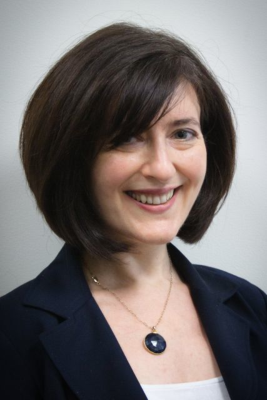
\includegraphics[height=100px]{content/day2/kuperberg-headshot.pdf}
\end{center}

\noindent
{\bfseries Abstract:} It is well established that we draw upon our real-world knowledge to predict
upcoming events and even individual words. I will discuss evidence that the neurocognitive
mechanisms that we engage in retrieving conceptual information associated with incoming words are
quite distinct from those engaged when these predictions are disconfirmed by the input. Drawing
broad links with computational models conceptualizing language comprehension as an incremental
process of belief updating, I will suggest that the engagement of these distinct neurocognitive
systems allows for comprehension that is both highly efficient and highly flexible (1).

I will first discuss studies using event-related potentials (ERPs) to examine online brain activity
during sentence and discourse comprehension. I will then draw some (still tentative) links between
this ERP literature and some relevant fMRI and MEG studies. Finally, I will discuss the advantages
of a predictive comprehension system. Predicting correctly clearly offers advantages in terms of
computational efficiency. Here I will argue that the costs incurred when we predict incorrectly are
also crucial for successful and flexible comprehension. Neurocognitive responses triggered by
prediction errors may rescue us from interpretation errors in noisy environments, may allow us learn
novel events, and may enable us to flexibly adjust our comprehension strategies in response to
everchanging task and environmental demands.

\vspace{3em}\par 

\vfill
\noindent
{\bfseries Biography}: Gina R Kuperberg is a Cognitive Neuroscientist and a Professor in the
Department of Psychology and the Cognitive Science Center at Tufts University, Boston. She is also a
Board Certified Psychiatrist and a Principal Investigator in the Psychiatry Neuroscience Program at
Massachusetts General Hospital, Harvard Medical School. Her research program aims to understand the
neurocognitive mechanisms by which the human brain builds meaning from language, and how these
mechanisms break down in neuropsychiatric disorders, particularly schizophrenia.

Dr.\ Kuperberg's Lab is situated across in both the Department of Psychology at Tufts and the
Martinos Center for Biomedical Imaging at Massachusetts General Hospital. The Lab uses multimodal
neuroimaging methods –– event-related potentials (ERPs), functional MRI (fMRI) and
magneto-encephalography (MEG) –– to probe both the spatial and temporal dimensions of cognition in
the brain. Her research program is funded by an RO1 from the National Institute of Mental Health
(NIMH), as well as awards from the Brain and Behavior Research Foundation and the Sidney Baer
Trust. She, her students, postdocs and collaborators publish in a wide range of journals of
Cognitive Neuroscience, Psycholinguistics, Experimental Psychology, Neuroimaging and Psychiatry.

Dr.\ Kuperberg has served as a standing member for the Language and Communication Study Section for
the National Institute of Health, and as a committee representative for Language for the Cognitive
Neuroscience society. Her research accomplishments have been recognized by several awards, including
the A.E. Bennett Research Award from the Society for Biological Psychiatry, the Joseph Zubin Award
for Significant Contributions to Research in Psychopathology, and an Award from Brain Research for
their most highly cited article, for her review of the architecture of the language system, Neural
Mechanisms of Language Comprehension: Challenges to Syntax.

Dr.\ Kuperberg earned her MD at St. Bartholomew's Medical School, London, and her PhD in Psychology
and Cognitive Neuroscience at Kings College, University of London. She completed an internship at
St. Bartholomew's Hospital and residency training in Psychiatry at the Maudsley Hospital and
Institute of Psychiatry, London. In 1998, she came to Boston where she completed research
fellowships in Neuroimaging and Cognitive Electrophysiology at Massachusetts General Hospital,
Harvard Medical School and Tufts University, working with David Caplan, Anders Dale and Phil
Holcomb.
\newpage
\newpage

%\section{Oral Presentations}
%\vspace{1em}\par\centerline{\bfseries\Large Paper Abstracts}\vspace{1em}\par
%% \addcontentsline{toc}{section}{Session 1}
\clearpage
\par\centerline{\bfseries\large Session M1a: Machine Translation}\vspace{1em}\par
\paperabstract{Monday}{10:40am--11:05am}{garbage}{garbage}{main-268}
\paperabstract{Monday}{11:05am--11:30am}{garbage}{garbage}{main-319}
\paperabstract{Monday}{11:30am--11:55am}{garbage}{garbage}{main-276}
\paperabstract{Monday}{11:55am--12:20pm}{garbage}{garbage}{main-419}
\clearpage
\par\centerline{\bfseries\large Session M1b: Information Extraction}\vspace{1em}\par
\paperabstract{Monday}{10:40am--11:05am}{garbage}{garbage}{main-441}
\paperabstract{Monday}{11:05am--11:30am}{garbage}{garbage}{main-282}
\paperabstract{Monday}{11:30am--11:55am}{garbage}{garbage}{main-174}
\paperabstract{Monday}{11:55am--12:20pm}{garbage}{garbage}{main-125}
\clearpage
\par\centerline{\bfseries\large Session M1c: Cognitive and Psycholinguistics}\vspace{1em}\par
\paperabstract{Monday}{10:40am--11:05am}{garbage}{garbage}{main-377}
\paperabstract{Monday}{11:05am--11:30am}{garbage}{garbage}{main-474}
\paperabstract{Monday}{11:30am--11:55am}{garbage}{garbage}{main-082}
\paperabstract{Monday}{11:55am--12:20pm}{garbage}{garbage}{main-370}
\clearpage
\par\centerline{\bfseries\large Session M2a: Parsing and Syntax}\vspace{1em}\par
\paperabstract{Monday}{2:00pm--2:25pm}{garbage}{garbage}{main-233}
\paperabstract{Monday}{2:25pm--2:50pm}{garbage}{garbage}{main-002}
\paperabstract{Monday}{2:50pm--3:15pm}{garbage}{garbage}{main-239}
\paperabstract{Monday}{3:15pm--3:40pm}{garbage}{garbage}{TACL-001}
\clearpage
\par\centerline{\bfseries\large Session M2b: Topic Modeling and Text Mining}\vspace{1em}\par
\paperabstract{Monday}{2:00pm--2:25pm}{garbage}{garbage}{main-266}
\paperabstract{Monday}{2:25pm--2:50pm}{garbage}{garbage}{main-317}
\paperabstract{Monday}{2:50pm--3:15pm}{garbage}{garbage}{main-308}
\paperabstract{Monday}{3:15pm--3:40pm}{garbage}{garbage}{main-155}
\clearpage
\par\centerline{\bfseries\large Session M2c: Spoken Language Processing}\vspace{1em}\par
\paperabstract{Monday}{2:00pm--2:25pm}{garbage}{garbage}{main-363}
\paperabstract{Monday}{2:25pm--2:50pm}{garbage}{garbage}{main-429}
\paperabstract{Monday}{2:50pm--3:15pm}{garbage}{garbage}{main-438}
\paperabstract{Monday}{3:15pm--3:40pm}{garbage}{garbage}{main-361}

\newpage

% I'm bypassing the \section command here because I didn't like the layout
% from the ACL-IJNLP handbook that I started from. UG

\setheaders{NAACL HLT: Poster and Demonstrations Session}{Monday, June 10, 2013}

\vspace{1em}\par\centerline{\bfseries\Large Poster Madness!}\vspace{1em}\par
\addcontentsline{toc}{section}{Poster madness!}

Prior to the poster session, poster presenters are given one minute each to pitch their
paper. Posters from the Student Research Workshop are included. Following the Poster Madness!
session, there will be a buffet dinner and a combined Posters and Demonstrations session.

\noindent
\vspace{1em}\par\centerline{\bfseries\large Main Conference Posters}\vspace{1em}\par
\posterabstract{main-180}
\posterabstract{main-393}
\posterabstract{main-345}
\posterabstract{main-108}
\posterabstract{main-195}
\posterabstract{main-410}
\posterabstract{main-020}
\posterabstract{main-206}
\posterabstract{main-089}
\posterabstract{main-420}
\posterabstract{TACL-002}
\posterabstract{main-289}
\posterabstract{main-184}
\posterabstract{main-293}
\posterabstract{main-120}
\posterabstract{main-390}
\posterabstract{main-431}
\posterabstract{main-137}
\posterabstract{main-457}
\posterabstract{main-336}
\posterabstract{main-402}
\posterabstract{main-075}
\posterabstract{main-385}
\posterabstract{main-300}
\posterabstract{main-128}
\posterabstract{main-264}
\posterabstract{main-278}
\posterabstract{main-397}
\posterabstract{main-212}
\posterabstract{main-250}
\posterabstract{main-313}
\posterabstract{main-351}
\posterabstract{main-225}
\posterabstract{main-340}
\posterabstract{main-023}
\posterabstract{main-446}
\posterabstract{main-004}
\posterabstract{main-372}
\posterabstract{main-066}
\posterabstract{main-449}
\posterabstract{main-095}
\posterabstract{main-057}
\posterabstract{main-283}
\posterabstract{main-275}
\posterabstract{main-467}
\posterabstract{main-070}
\posterabstract{main-221}
\posterabstract{main-072}


\noindent
\vspace{1em}\par\centerline{\bfseries\large Student Research Workshop Posters}\vspace{1em}\par
\noindent
%% \posterentry{srw-005}\\[1ex]
\posterentry{srw-020}\\[1ex]
\posterentry{srw-008}\\[1ex]
\posterentry{srw-007}\\[1ex]
\posterentry{srw-002}\\[1ex]
\posterentry{srw-010}\\[1ex]
\posterentry{srw-018}\\[1ex]
\posterentry{srw-015}\\[1ex]
\posterentry{srw-024}\\[1ex]
\posterentry{srw-016}\\[1ex]
\posterentry{srw-014}\\[1ex]
\posterentry{srw-012}\\[1ex]
\posterentry{srw-021}\\[1ex]

\posterabstract{srw-002}\par
\posterabstract{srw-005}\par
\posterabstract{srw-007}\par
\posterabstract{srw-008}\par
\posterabstract{srw-010}\par
\posterabstract{srw-012}\par
\posterabstract{srw-014}\par
\posterabstract{srw-015}\par
\posterabstract{srw-016}\par
\posterabstract{srw-018}\par
\posterabstract{srw-020}\par
\posterabstract{srw-021}\par
\posterabstract{srw-024}\par


\noindent
\vspace{1em}\par\centerline{\bfseries\large Demonstrations}\vspace{1em}\par
\addcontentsline{toc}{section}{Poster and Demonstrations Session}

Demonstrations will be held during the Poster and Demonstrations Session, but are not part of the
Poster Madness!

\noindent
%% \posterentry{demo-001}\\[1ex]
\posterentry{demo-002}\\[1ex]
\posterentry{demo-004}\\[1ex]
\posterentry{demo-006}\\[1ex]
\posterentry{demo-008}\\[1ex]
\posterentry{demo-009}\\[1ex]
\posterentry{demo-012}\\[1ex]
\posterentry{demo-015}\\[1ex]
\posterentry{demo-016}\\[1ex]

\paperabstract{Monday}{6:00pm--9:00pm}{Poster Session}{\PosterSessionLoc}{demo-001}\par
\paperabstract{Monday}{6:00pm--9:00pm}{Poster Session}{\PosterSessionLoc}{demo-002}\par
\paperabstract{Monday}{6:00pm--9:00pm}{Poster Session}{\PosterSessionLoc}{demo-004}\par
\paperabstract{Monday}{6:00pm--9:00pm}{Poster Session}{\PosterSessionLoc}{demo-006}\par
\paperabstract{Monday}{6:00pm--9:00pm}{Poster Session}{\PosterSessionLoc}{demo-008}\par
\paperabstract{Monday}{6:00pm--9:00pm}{Poster Session}{\PosterSessionLoc}{demo-009}\par
\paperabstract{Monday}{6:00pm--9:00pm}{Poster Session}{\PosterSessionLoc}{demo-012}\par
\paperabstract{Monday}{6:00pm--9:00pm}{Poster Session}{\PosterSessionLoc}{demo-015}\par
\paperabstract{Monday}{6:00pm--9:00pm}{Poster Session}{\PosterSessionLoc}{demo-016}\par


%\mbox{}\vspace*{-5cm}\par

\chapter{Tuesday, June 5, 2012: Main Conference}
\thispagestyle{emptyheader}
\setheaders{NAACL HLT Main Conference}{Tuesday, June 5, 2012}
%\vspace{-.5cm}
\section*{Overview}
\renewcommand{\arraystretch}{1.2}
\begin{SingleTrackSchedule}
 7:00am & -- & 6:00pm &
 {\bfseries Registration} \hfill (\RegLoc)
 \\

 7:30am & -- & 9:00am &
 {\bfseries Continental Breakfast} \hfill (\BreakfastLoc)
 \\

  9:15am & -- &  10:15am & 
  {\bfseries Best Paper Awards Session} \hfill (\PBLRM)
  \\[1ex]%\hline[-2ex]

  10:15am & -- & 10:45am & \bfseries Break \hfill (\BreakLoc)
  \\[1ex]%\hline[-2ex]

  10:45am & -- & 12:00pm & 
  {\bfseries Parallel Sessions: Short papers}\newline
  \hfill \emph{Machine Translation and Multilinguality} \hfill (\PBC)\newline
  \hfill \emph{Sentiment Analysis and Topic Modeling} \hfill (\PLZBLRM)\newline
  \hfill \emph{Spoken Language Processing} \hfill (\PDE)
  \\[1ex]%\hline[-2ex]
  
  12:00pm & -- & 2:00pm & 
  {\bfseries Lunch}\hfill
  \\[1ex]%\hline[-2ex]

  1:00pm & -- & 2:00pm & 
  {\bfseries Business Meeting}\hfill (\PBC)\newline
  \hfill \emph{All are welcome!}
  \\[1ex]%\hline[-2ex]

  2:00pm & -- & 3:15pm & 
  {\bfseries Parallel Sessions: Short papers}\newline
  \hfill \emph{Semantics} \hfill (\PBC)\newline
  \hfill \emph{Information Extraction} \hfill (\PLZBLRM)\newline
  \hfill \emph{Discourse and Dialog		} \hfill (\PDE)
  \\[1ex]%\hline[-2ex]

  3:15pm & -- & 3:45pm & 
  \bfseries Break \hfill (\BreakLoc)
  \\[1ex]%\hline[-2ex]

  3:45pm & -- & 5:25pm & 
  {\bfseries Parallel Sessions}\newline
  \hfill \emph{Semantics} \hfill (\PBC)\newline
  \hfill \emph{Information Extraction} \hfill (\PLZBLRM)\newline
  \hfill \emph{Discourse} \hfill (\PDE)
  \\[1ex]%\hline[-2ex]

  7:00pm & -- & 11:00pm & 
  \bfseries Banquet at World of Coca-Cola Museum

\end{SingleTrackSchedule}

%%\begin{landscape}
%\vspace*{-.75cm}
\begin{landscape}
%\mbox{}\vfill 
\noindent
\begin{FourTrackSchedule}
\multicolumn{7}{c}{\bfseries\Large Schedule}\\\hline
\hline\BreakTime{7:30am}{5:00pm}{4}{Registration (\FOY)}\\\hline\noalign{\smallskip}
%\multicolumn{6}{c}{\ }\\[.25ex]
\hline
\BreakTime   {7:30am}{9:00am}{4}{Breakfast (\FOY)}\\\hline
\PlenaryEvent{9:00am}{10:30am}{4}{
{\bfseries Best Paper Awards (\PLN)}\linebreak
\small{\bfseries Chair:} {\textnormal{\itshape Eric Fosler-Lussier}}) } \\\hline

\PlenaryEvent{9:00am}{9:30am}{4}{\paperentry{main-062}}\\\hline
\PlenaryEvent{9:30am}{10:00am}{4}{\paperentry{main-054}}\\\hline
\PlenaryEvent{10:00am}{10:30am}{4}{\paperentry{main-101}}\\\hline
%\multicolumn{3}{|c|}{$\downarrow$}&\multicolumn{4}{c|}{$\downarrow$}\\
%\end{FourTrackSchedule}


%\begin{FourTrackSchedule}
%\multicolumn{3}{|c|}{$\vdots$} & \multicolumn{4}{c|@{}}{$\vdots$}\\

\BreakTime{10:30am}{11:00am}{4}{Coffee Break (\FOY)}\\\hline
\multicolumn{3}{|c|}{\bfseries Parallel Sessions}
& \bfseries East Ballroom
& \bfseries Center Ballroom
& \bfseries West Ballroom
& \bfseries Drummond
\\\hline

\bfseries 11:00am & -- & \bfseries 12:30pm
& \bfseries \PM 
& \bfseries \MT~II  
& \bfseries \SM~I 
& \bfseries \SP  
\\
&&
& {\small {\bfseries Chair:} {\itshape T.B.D.}} 
& {\small {\bfseries Chair:} {\itshape Chris Callison-Burch}} 
& {\small {\bfseries Chair:} {\itshape Chris Brew}} 
& {\small {\bfseries Chair:} {\itshape Noah Smith}}\\\hline
10:45am & -- & 11:00am & \paperentry{main-047}\\\hline
11:00am & -- & 11:15am & \paperentry{main-022}\\\hline
11:15am & -- & 11:30am & \paperentry{main-444}\\\hline
11:30am & -- & 11:45am & \paperentry{main-392}\\\hline
11:45am & -- & 12:00pm & \paperentry{main-071}\\\hline
10:45am & -- & 11:00am & \paperentry{main-016}\\\hline
11:00am & -- & 11:15am & \paperentry{main-106}\\\hline
11:15am & -- & 11:30am & \paperentry{main-400}\\\hline
11:30am & -- & 11:45am & \paperentry{main-310}\\\hline
11:45am & -- & 12:00pm & \paperentry{main-314}\\\hline
10:45am & -- & 11:00am & \paperentry{main-329}\\\hline
11:00am & -- & 11:15am & \paperentry{main-404}\\\hline
11:15am & -- & 11:30am & \paperentry{main-455}\\\hline
11:30am & -- & 11:45am & \paperentry{main-442}\\\hline
11:45am & -- & 12:00pm & \paperentry{main-353}\\\hline
\hline
\BreakTime{12:30pm}{2:00pm}{4}{Lunch Break}\\\hline
\end{FourTrackSchedule}
\end{landscape}\pagebreak
\noindent
\begin{landscape}
\noindent
\begin{FourTrackSchedule}\hline
\PlenaryEvent{2:00pm}{3:30pm}{4}{%
\index{Charniak, Eugene}\index{Hirst, Graeme}\index{Mooney, Ray}%
\index{Ostendorf, Mari}\index{Eisner, Jason}\index{Resnik, Philip}%
\index{Vanderwende, Lucy}\renewcommand{\baselinestretch}{1}%
\centering
{\bfseries\rule{0pt}{2.5ex} NLP Idol: Plucked from Obscurity (\CBR)} 
\linebreak
\normalfont\small
{\itshape Eugene Charniak, Graeme Hirst, Ray Mooney,} and {\itshape
  Mari Ostendorf $\dots$}\linebreak
$\dots$ have dug out papers from the past that they think should still get us excited today.\linebreak Come and see
what they've brought for show and tell! Can they convince the
judges?\vspace{.5ex}\linebreak
{\bfseries Moderator:} {\itshape Brian Roark} \hspace{1em}
{\bfseries Judges:} {\itshape Jason Eisner, Philip Resnik, Lucy Vanderwende}}%\\
\\\hline

\BreakTime{3:30pm}{4:00pm}{4}{Coffee Break (\FOY)}\\\hline

\multicolumn{3}{|c|}{\bfseries Parallel Sessions}
& \bfseries East Ballroom
& \bfseries Center Ballroom
& \bfseries West Ballroom
& \bfseries Drummond
\\\hline

\multicolumn{3}{|c|}{\bfseries Short Papers}
& \bfseries \DC 
& \bfseries \MT  
& \bfseries \CTM  
& \bfseries Syntax  
\\
&&
& {\small {\bfseries Chair:} {\itshape Vincent Ng}} 
& {\small {\bfseries Chair:} {\itshape George Foster}} 
& {\small {\bfseries Chair:} {\itshape Diana Inkpen}} 
& {\small {\bfseries Chair:} {\itshape Chris Manning}} 
\\\hline

2:00pm & -- & 2:15pm & \paperentry{main-001}\\\hline
2:15pm & -- & 2:30pm & \paperentry{main-119}\\\hline
2:30pm & -- & 2:45pm & \paperentry{main-037}\\\hline
2:45pm & -- & 3:00pm & \paperentry{main-197}\\\hline
3:00pm & -- & 3:15pm & \paperentry{main-434}\\\hline
2:00pm & -- & 2:15pm & \paperentry{main-114}\\\hline
2:15pm & -- & 2:30pm & \paperentry{main-046}\\\hline
2:30pm & -- & 2:45pm & \paperentry{main-163}\\\hline
2:45pm & -- & 3:00pm & \paperentry{main-417}\\\hline
3:00pm & -- & 3:15pm & \paperentry{main-375}\\\hline
2:00pm & -- & 2:15pm & \paperentry{main-292}\\\hline
2:15pm & -- & 2:30pm & \paperentry{main-462}\\\hline
2:30pm & -- & 2:45pm & \paperentry{main-098}\\\hline
2:45pm & -- & 3:00pm & \paperentry{main-274}\\\hline
3:00pm & -- & 3:15pm & \paperentry{main-160}\\\hline


\BreakTime{7:00pm}{late}{4}{Banquet at Le Windsor Ballroom}\\\hline
\end{FourTrackSchedule}
\vfill
\end{landscape}

\newpage

%\section[]{Best Paper Awards Session}
\noindent
\vspace{1em}\par\centerline{\bfseries\Large Best Paper Awards}\vspace{1em}\par
\addcontentsline{toc}{section}{Best Paper Awards}

\paperabstract{Tuesday}{9:25am--9:45am}{\Btitle}{\PBLRM}{main-027}
\paperabstract{Tuesday}{9:45am--10:15am}{\Btitle}{\PBLRM}{main-332}

\clearpage
%\section{Banquet}
\noindent
\par
\addcontentsline{toc}{section}{Banquet Venue}
%\section{NAACL 2013 Banquet}
\begin{center}

\begin{Large}
{\bfseries\Large NAACL 2013 Banquet at World of Coca Cola}\vspace{1em}\par
\end{Large}

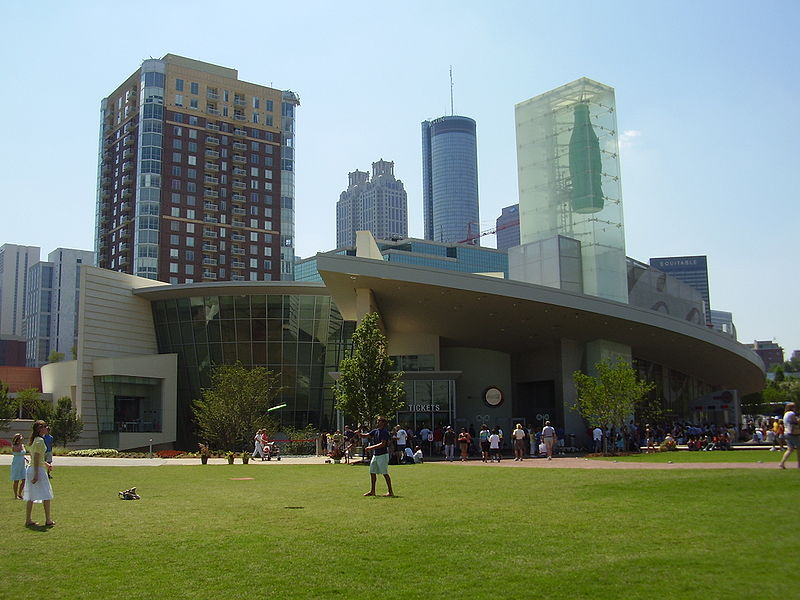
\includegraphics[height=100px]{content/day3/cocacola.jpg}

Tuesday, June 11, 2013, 7:00pm -- 9:00am \vspace{1em}\\
The World of Coca-Cola\\
121 Baker St. NW\\
Atlanta, GA 30313-1807\\
\end{center}

\noindent
This year's NAACL banquet promises to be a unique and interactive experience! Taking place in the intriguing World of Coca Cola Museum, attendees will have access to a multi-sensory 4D theater, an extraordinary 1880s soda fountain, the smallest bottling line in the world, plus an opportunity to sample nearly 70 different beverages from around the globe. Multiple buffet stations and seating areas will allow banquet-goers to enjoy the food and explore the museum at their leisure. And, of course there will be a DJ for your dancing pleasure. The banquet will take place at the World of Coca Cola Museum , Tuesday evening, June 11th. So, save yourselves the standard \$15-16 entrance fee and join us on Tuesday.


\newpage


\clearpage
%\section{Oral Presentations}
\noindent
\vspace{1em}\par\centerline{\bfseries\Large Paper Abstracts}\vspace{1em}\par
\addcontentsline{toc}{section}{Paper Abstracts}
\paperabstract{Tuesday}{10:45am--11:00am}{\Btitle}{\PBC}{main-047}
\paperabstract{Tuesday}{11:00am--11:15am}{\Btitle}{\PBC}{main-022}
\paperabstract{Tuesday}{11:15am--11:30am}{\Btitle}{\PBC}{main-444}
\paperabstract{Tuesday}{11:30am--11:45am}{\Btitle}{\PBC}{main-392}
\paperabstract{Tuesday}{11:45am--12:00pm}{\Btitle}{\PBC}{main-071}
\paperabstract{Tuesday}{10:45am--11:00am}{\Btitle}{\PLZBLRM}{main-016}
\paperabstract{Tuesday}{11:00am--11:15am}{\Btitle}{\PLZBLRM}{main-106}
\paperabstract{Tuesday}{11:15am--11:30am}{\Btitle}{\PLZBLRM}{main-400}
\paperabstract{Tuesday}{11:30am--11:45am}{\Btitle}{\PLZBLRM}{main-310}
\paperabstract{Tuesday}{11:45am--12:00pm}{\Btitle}{\PLZBLRM}{main-314}
\paperabstract{Tuesday}{10:45am--11:00am}{\Btitle}{\PDE}{main-329}
\paperabstract{Tuesday}{11:00am--11:15am}{\Btitle}{\PDE}{main-404}
\paperabstract{Tuesday}{11:15am--11:30am}{\Btitle}{\PDE}{main-455}
\paperabstract{Tuesday}{11:30am--11:45am}{\Btitle}{\PDE}{main-442}
\paperabstract{Tuesday}{11:45am--12:00pm}{\Btitle}{\PDE}{main-353}

\paperabstract{Tuesday}{2:00pm--2:15pm}{\Btitle}{\PBC}{main-001}
\paperabstract{Tuesday}{2:15pm--2:30pm}{\Btitle}{\PBC}{main-119}
\paperabstract{Tuesday}{2:30pm--2:45pm}{\Btitle}{\PBC}{main-037}
\paperabstract{Tuesday}{2:45pm--3:00pm}{\Btitle}{\PBC}{main-197}
\paperabstract{Tuesday}{3:00pm--3:15pm}{\Btitle}{\PBC}{main-434}
\paperabstract{Tuesday}{2:00pm--2:15pm}{\Btitle}{\PLZBLRM}{main-114}
\paperabstract{Tuesday}{2:15pm--2:30pm}{\Btitle}{\PLZBLRM}{main-046}
\paperabstract{Tuesday}{2:30pm--2:45pm}{\Btitle}{\PLZBLRM}{main-163}
\paperabstract{Tuesday}{2:45pm--3:00pm}{\Btitle}{\PLZBLRM}{main-417}
\paperabstract{Tuesday}{3:00pm--3:15pm}{\Btitle}{\PLZBLRM}{main-375}
\paperabstract{Tuesday}{2:00pm--2:15pm}{\Btitle}{\PDE}{main-292}
\paperabstract{Tuesday}{2:15pm--2:30pm}{\Btitle}{\PDE}{main-462}
\paperabstract{Tuesday}{2:30pm--2:45pm}{\Btitle}{\PDE}{main-098}
\paperabstract{Tuesday}{2:45pm--3:00pm}{\Btitle}{\PDE}{main-274}
\paperabstract{Tuesday}{3:00pm--3:15pm}{\Btitle}{\PDE}{main-160}

\clearpage{\thispagestyle{emptyheader}\cleardoublepage}


\chapter{Wednesday, June 12, 2013: Main Conference}
\thispagestyle{emptyheader}
\setheaders{NAACL HLT Main Conference}{Wednesday, June 12, 2013}
\centerline{\bfseries\Large Overview}
\renewcommand{\arraystretch}{1.2}
\begin{SingleTrackSchedule}
 7:00am & -- & 6:00pm &
 {\bfseries Registration} \hfill (\RegLoc)
 \\

 7:30am & -- & 9:00am &
 {\bfseries Continental Breakfast} \hfill (\BreakfastLoc)
 \\

  9:00am & -- & 10:10am & 
  {\bfseries Invited Talk: Kathleen McKeown} \hfill (\ATLBRM)
  \\[1ex]%\hline[-2ex]

  10:10am & -- & 10:40am & {\bfseries Break} \hfill (\BreakLoc)
  \\[1ex]%\hline[-2ex]

  10:40am & -- & 12:20pm & 
  {\bfseries Parallel Sessions}\newline
  \hfill \emph{Machine Translation} \hfill (\MOaLoc)\newline
  \hfill \emph{Semantics} \hfill (\MObLoc)\newline
  \hfill \emph{Social Media Processing} \hfill (\MOcLoc)
  \\[1ex]%\hline[-2ex]
  
  12:20pm & -- & 2:00pm & 
  \bfseries Lunch
  \\[1ex]%\hline[-2ex]

  2:00pm & -- & 3:15pm & 
  {\bfseries Parallel Sessions}\newline
  \hfill \emph{Parsing and Syntax} \hfill (\MOaLoc)\newline
  \hfill \emph{Dialog} \hfill (\MObLoc)\newline
  \hfill \emph{Annotation and Language Resources} \hfill (\MOcLoc)
  \\[1ex]%\hline[-2ex]

  3:15pm & -- & 3:45pm & 
     {\bfseries Break} \hfill (\BreakLoc)
  \\[1ex]%\hline[-2ex]

  3:45pm & -- & 5:00pm & 
  {\bfseries Parallel Sessions}\newline
  \hfill \emph{Semantics and Syntax} \hfill (\MOaLoc)\newline
  \hfill \emph{Summarization and Generation} \hfill (\MObLoc)\newline
  \hfill \emph{Morphology and Phonology} \hfill (\MOcLoc)
  \\[1ex]%\hline[-2ex]

  5:00pm & & & 
  \bfseries Conference adjourns!
  \\[1ex]%\hline[-2ex]

\end{SingleTrackSchedule}

\newpage
%\begin{landscape}
\centerline{\bfseries\Large Schedule}%\vspace{2ex}

\noindent
\begin{ThreeTrackSchedule}
\hline\BreakTime{7:30am}{5:00pm}{3}{Registration (\FOY)}\\\hline\noalign{\bigskip}
%\multicolumn{6}{c}{\ }\\[.25ex]
\hline
\BreakTime   {7:30am}{9:00am}{3}{Breakfast (\FOY)}\\\hline
\PlenaryEvent{9:00am}{10:15am}{3}{{\bfseries Invited Talk (\PLN)}\linebreak
{\itshape J. W. Pennebaker:} {``A, is, I, and, the: How our smallest words reveal the most about who we Are''}\linebreak{\small {\bfseries Chair:} by {\itshape Srinivas Bangalore}}}\\\hline
\BreakTime{10:15am}{10:40am}{3}{Coffee Break (\FOY)}\\\hline

\multicolumn{3}{|c|}{\bfseries Parallel Sessions}
& \bfseries East Ballroom
& \bfseries Center Ballroom
& \bfseries West Ballroom
\\\hline

\multicolumn{3}{|c|}{\bfseries Short Papers}
& \bfseries \SSM 
& \bfseries \SM  
& \bfseries \SU  
\\
&&
& {\small {\bfseries Chair:} {\itshape Theresa Wilson}} 
& {\small {\bfseries Chair:} {\itshape Phil Resnik}} 
& {\small {\bfseries Chair:} {\itshape Ani Nenkova}} 
\\\hline

\input{auto/main/wednesday-main-1}

\end{ThreeTrackSchedule}

\clearpage

\begin{ThreeTrackSchedule}

\hline
\BreakTime{12:00pm}{1:00pm}{3}{Lunch Break}\\\hline

\PlenaryEvent{1:00pm}{2:00pm}{3}{%
{\bfseries NAACL Business Meeting (open to all; \CBR)}}\\\hline

\multicolumn{3}{|c|}{\bfseries Parallel Sessions}
& \bfseries East Ballroom
& \bfseries Center Ballroom
& \bfseries West Ballroom
\\\hline

%\bfseries 2:30pm & -- & \bfseries 4:00pm
&&
& \bfseries \SSM  
& \bfseries \ML~II 
& \bfseries \DDP~II \\
&&
& {\small {\bfseries Chair:} {\itshape Saif Mohammed}} 
& {\small {\bfseries Chair:} {\itshape Scott Yih}} 
& {\small {\bfseries Chair:} {\itshape Diane Litman}} 
\\\hline

\input{auto/main/wednesday-main-2}

\BreakTime{3:40pm}{4:10pm}{3}{Coffee Break (\FOY)}\\\hline

\multicolumn{3}{|c|}{\bfseries Parallel Sessions}
& \bfseries East Ballroom
& \bfseries Center Ballroom
& \bfseries West Ballroom
\\\hline

%\bfseries 2:30pm & -- & \bfseries 4:00pm
&&
& \bfseries \SU  
& \bfseries \SM~II 
& \bfseries \CTM \\
&&
& {\small {\bfseries Chair:} {\itshape Advaith Siddharthan}} 
& {\small {\bfseries Chair:} {\itshape Mona Diab}} 
& {\small {\bfseries Chair:} {\itshape Ryan McDonald}}
\\\hline
\input{auto/main/wednesday-main-3}
\end{ThreeTrackSchedule}
\end{landscape}

%\thispagestyle{myheadings}
\section{Invited Talk: Kathleen McKeown}
\index{McKeown, Kathleen}
\begin{center}
%% --- Keynote Address ---
%% \vspace{2em}\\
%% \vfill

\begin{Large}
{\bfseries\Large ``Natural Language Applications from Fact to Fiction''}\vspace{1em}\par
\end{Large}

{\itshape Kathleen McKeown}\vspace{1em}\par
Wednesday, June 12, 2013, 9:00am -- 10:10am \vspace{1em}\\
\PlenaryLoc
\end{center}

\noindent
{\bfseries Abstract:} Much research in the natural language field has been carried out on news, given the large amount of annotated data now available for this genre.

Certainly, the ability to analyze the facts of real world events, enabling systems to answer questions and summarize the events of the day is an important application. As research has moved to analysis of new genres, whether fact, opinion or fiction, new approaches to existing applications have arisen and opportunities for new applications have emerged. In this talk, I will present research in my group at Columbia as it has moved from news to scientific articles to online discussion forums to novels. I will touch on summarization, open-ended question answering, social influence and social networks.

\vspace{3em}\par 

\vfill
\noindent
{\bfseries Biography:} A leading scholar and researcher in the field of natural language processing,
McKeown focuses her research on big data; her interests include text summarization, question
answering, natural language generation, multimedia explanation, digital libraries, and multilingual
applications. Her research group's Columbia Newsblaster, which has been live since 2001, is an
online system that automatically tracks the day's news, and demonstrates the group's new
technologies for multi-document summarization, clustering, and text categorization, among
others. Currently, she leads a large research project involving prediction of technology emergence
from a large collection of journal articles.

McKeown joined Columbia in 1982, immediately after earning her Ph.D. from University of Pennsylvania. In 1989, she became the first woman professor in the school to receive tenure, and later the first woman to serve as a department chair (1998-2003). McKeown has received numerous honors and awards for her research and teaching. She received the National Science Foundation Presidential Young Investigator Award in 1985, and also is the recipient of a National Science Foundation Faculty Award for Women, was selected as an AAAI Fellow, a Founding Fellow of the Association for Computational Linguistics and an ACM Fellow. In 2010, she won both the Columbia Great Teacher Award—an honor bestowed by the students—and the Anita Borg Woman of Vision Award for Innovation.

McKeown served as a board member of the Computing Research Association and as secretary of the board. She was president of the Association of Computational Linguistics in 1992, vice president in 1991, and secretary treasurer for 1995-1997. She was also a member of the Executive Council of the Association for Artificial Intelligence and the co-program chair of their annual conference in 1991.

\newpage

\newpage

%\section{Oral Presentations}
\vspace{1em}\par\centerline{\bfseries\Large Paper Abstracts}\vspace{1em}\par
\addcontentsline{toc}{section}{Paper Abstracts}
\input{auto/main/wednesday-main-1-B-abstracts.tex}
\input{auto/main/wednesday-main-2-B-abstracts.tex}
\input{auto/main/wednesday-main-3-B-abstracts.tex}
\clearpage{\thispagestyle{emptyheader}\cleardoublepage}


%%\mbox{}\vspace*{-5cm}\par

\chapter{Tuesday, June 5, 2012: Main Conference}
\thispagestyle{emptyheader}
\setheaders{NAACL HLT Main Conference}{Tuesday, June 5, 2012}
%\vspace{-.5cm}
\section*{Overview}
\renewcommand{\arraystretch}{1.2}
\begin{SingleTrackSchedule}
 7:00am & -- & 6:00pm &
 {\bfseries Registration} \hfill (\RegLoc)
 \\

 7:30am & -- & 9:00am &
 {\bfseries Continental Breakfast} \hfill (\BreakfastLoc)
 \\

  9:15am & -- &  10:15am & 
  {\bfseries Best Paper Awards Session} \hfill (\PBLRM)
  \\[1ex]%\hline[-2ex]

  10:15am & -- & 10:45am & \bfseries Break \hfill (\BreakLoc)
  \\[1ex]%\hline[-2ex]

  10:45am & -- & 12:00pm & 
  {\bfseries Parallel Sessions: Short papers}\newline
  \hfill \emph{Machine Translation and Multilinguality} \hfill (\PBC)\newline
  \hfill \emph{Sentiment Analysis and Topic Modeling} \hfill (\PLZBLRM)\newline
  \hfill \emph{Spoken Language Processing} \hfill (\PDE)
  \\[1ex]%\hline[-2ex]
  
  12:00pm & -- & 2:00pm & 
  {\bfseries Lunch}\hfill
  \\[1ex]%\hline[-2ex]

  1:00pm & -- & 2:00pm & 
  {\bfseries Business Meeting}\hfill (\PBC)\newline
  \hfill \emph{All are welcome!}
  \\[1ex]%\hline[-2ex]

  2:00pm & -- & 3:15pm & 
  {\bfseries Parallel Sessions: Short papers}\newline
  \hfill \emph{Semantics} \hfill (\PBC)\newline
  \hfill \emph{Information Extraction} \hfill (\PLZBLRM)\newline
  \hfill \emph{Discourse and Dialog		} \hfill (\PDE)
  \\[1ex]%\hline[-2ex]

  3:15pm & -- & 3:45pm & 
  \bfseries Break \hfill (\BreakLoc)
  \\[1ex]%\hline[-2ex]

  3:45pm & -- & 5:25pm & 
  {\bfseries Parallel Sessions}\newline
  \hfill \emph{Semantics} \hfill (\PBC)\newline
  \hfill \emph{Information Extraction} \hfill (\PLZBLRM)\newline
  \hfill \emph{Discourse} \hfill (\PDE)
  \\[1ex]%\hline[-2ex]

  7:00pm & -- & 11:00pm & 
  \bfseries Banquet at World of Coca-Cola Museum

\end{SingleTrackSchedule}

%%\begin{landscape}
%\vspace*{-.75cm}
\begin{landscape}
%\mbox{}\vfill 
\noindent
\begin{FourTrackSchedule}
\multicolumn{7}{c}{\bfseries\Large Schedule}\\\hline
\hline\BreakTime{7:30am}{5:00pm}{4}{Registration (\FOY)}\\\hline\noalign{\smallskip}
%\multicolumn{6}{c}{\ }\\[.25ex]
\hline
\BreakTime   {7:30am}{9:00am}{4}{Breakfast (\FOY)}\\\hline
\PlenaryEvent{9:00am}{10:30am}{4}{
{\bfseries Best Paper Awards (\PLN)}\linebreak
\small{\bfseries Chair:} {\textnormal{\itshape Eric Fosler-Lussier}}) } \\\hline

\PlenaryEvent{9:00am}{9:30am}{4}{\paperentry{main-062}}\\\hline
\PlenaryEvent{9:30am}{10:00am}{4}{\paperentry{main-054}}\\\hline
\PlenaryEvent{10:00am}{10:30am}{4}{\paperentry{main-101}}\\\hline
%\multicolumn{3}{|c|}{$\downarrow$}&\multicolumn{4}{c|}{$\downarrow$}\\
%\end{FourTrackSchedule}


%\begin{FourTrackSchedule}
%\multicolumn{3}{|c|}{$\vdots$} & \multicolumn{4}{c|@{}}{$\vdots$}\\

\BreakTime{10:30am}{11:00am}{4}{Coffee Break (\FOY)}\\\hline
\multicolumn{3}{|c|}{\bfseries Parallel Sessions}
& \bfseries East Ballroom
& \bfseries Center Ballroom
& \bfseries West Ballroom
& \bfseries Drummond
\\\hline

\bfseries 11:00am & -- & \bfseries 12:30pm
& \bfseries \PM 
& \bfseries \MT~II  
& \bfseries \SM~I 
& \bfseries \SP  
\\
&&
& {\small {\bfseries Chair:} {\itshape T.B.D.}} 
& {\small {\bfseries Chair:} {\itshape Chris Callison-Burch}} 
& {\small {\bfseries Chair:} {\itshape Chris Brew}} 
& {\small {\bfseries Chair:} {\itshape Noah Smith}}\\\hline
10:45am & -- & 11:00am & \paperentry{main-047}\\\hline
11:00am & -- & 11:15am & \paperentry{main-022}\\\hline
11:15am & -- & 11:30am & \paperentry{main-444}\\\hline
11:30am & -- & 11:45am & \paperentry{main-392}\\\hline
11:45am & -- & 12:00pm & \paperentry{main-071}\\\hline
10:45am & -- & 11:00am & \paperentry{main-016}\\\hline
11:00am & -- & 11:15am & \paperentry{main-106}\\\hline
11:15am & -- & 11:30am & \paperentry{main-400}\\\hline
11:30am & -- & 11:45am & \paperentry{main-310}\\\hline
11:45am & -- & 12:00pm & \paperentry{main-314}\\\hline
10:45am & -- & 11:00am & \paperentry{main-329}\\\hline
11:00am & -- & 11:15am & \paperentry{main-404}\\\hline
11:15am & -- & 11:30am & \paperentry{main-455}\\\hline
11:30am & -- & 11:45am & \paperentry{main-442}\\\hline
11:45am & -- & 12:00pm & \paperentry{main-353}\\\hline
\hline
\BreakTime{12:30pm}{2:00pm}{4}{Lunch Break}\\\hline
\end{FourTrackSchedule}
\end{landscape}\pagebreak
\noindent
\begin{landscape}
\noindent
\begin{FourTrackSchedule}\hline
\PlenaryEvent{2:00pm}{3:30pm}{4}{%
\index{Charniak, Eugene}\index{Hirst, Graeme}\index{Mooney, Ray}%
\index{Ostendorf, Mari}\index{Eisner, Jason}\index{Resnik, Philip}%
\index{Vanderwende, Lucy}\renewcommand{\baselinestretch}{1}%
\centering
{\bfseries\rule{0pt}{2.5ex} NLP Idol: Plucked from Obscurity (\CBR)} 
\linebreak
\normalfont\small
{\itshape Eugene Charniak, Graeme Hirst, Ray Mooney,} and {\itshape
  Mari Ostendorf $\dots$}\linebreak
$\dots$ have dug out papers from the past that they think should still get us excited today.\linebreak Come and see
what they've brought for show and tell! Can they convince the
judges?\vspace{.5ex}\linebreak
{\bfseries Moderator:} {\itshape Brian Roark} \hspace{1em}
{\bfseries Judges:} {\itshape Jason Eisner, Philip Resnik, Lucy Vanderwende}}%\\
\\\hline

\BreakTime{3:30pm}{4:00pm}{4}{Coffee Break (\FOY)}\\\hline

\multicolumn{3}{|c|}{\bfseries Parallel Sessions}
& \bfseries East Ballroom
& \bfseries Center Ballroom
& \bfseries West Ballroom
& \bfseries Drummond
\\\hline

\multicolumn{3}{|c|}{\bfseries Short Papers}
& \bfseries \DC 
& \bfseries \MT  
& \bfseries \CTM  
& \bfseries Syntax  
\\
&&
& {\small {\bfseries Chair:} {\itshape Vincent Ng}} 
& {\small {\bfseries Chair:} {\itshape George Foster}} 
& {\small {\bfseries Chair:} {\itshape Diana Inkpen}} 
& {\small {\bfseries Chair:} {\itshape Chris Manning}} 
\\\hline

2:00pm & -- & 2:15pm & \paperentry{main-001}\\\hline
2:15pm & -- & 2:30pm & \paperentry{main-119}\\\hline
2:30pm & -- & 2:45pm & \paperentry{main-037}\\\hline
2:45pm & -- & 3:00pm & \paperentry{main-197}\\\hline
3:00pm & -- & 3:15pm & \paperentry{main-434}\\\hline
2:00pm & -- & 2:15pm & \paperentry{main-114}\\\hline
2:15pm & -- & 2:30pm & \paperentry{main-046}\\\hline
2:30pm & -- & 2:45pm & \paperentry{main-163}\\\hline
2:45pm & -- & 3:00pm & \paperentry{main-417}\\\hline
3:00pm & -- & 3:15pm & \paperentry{main-375}\\\hline
2:00pm & -- & 2:15pm & \paperentry{main-292}\\\hline
2:15pm & -- & 2:30pm & \paperentry{main-462}\\\hline
2:30pm & -- & 2:45pm & \paperentry{main-098}\\\hline
2:45pm & -- & 3:00pm & \paperentry{main-274}\\\hline
3:00pm & -- & 3:15pm & \paperentry{main-160}\\\hline


\BreakTime{7:00pm}{late}{4}{Banquet at Le Windsor Ballroom}\\\hline
\end{FourTrackSchedule}
\vfill
\end{landscape}

\newpage

%\section[]{Best Paper Awards Session}
\noindent
\vspace{1em}\par\centerline{\bfseries\Large Best Paper Awards}\vspace{1em}\par
\addcontentsline{toc}{section}{Best Paper Awards}

\paperabstract{Tuesday}{9:25am--9:45am}{\Btitle}{\PBLRM}{main-027}
\paperabstract{Tuesday}{9:45am--10:15am}{\Btitle}{\PBLRM}{main-332}

\clearpage
%\section{Banquet}
\noindent
\par
\addcontentsline{toc}{section}{Banquet Venue}
%\section{NAACL 2013 Banquet}
\begin{center}

\begin{Large}
{\bfseries\Large NAACL 2013 Banquet at World of Coca Cola}\vspace{1em}\par
\end{Large}

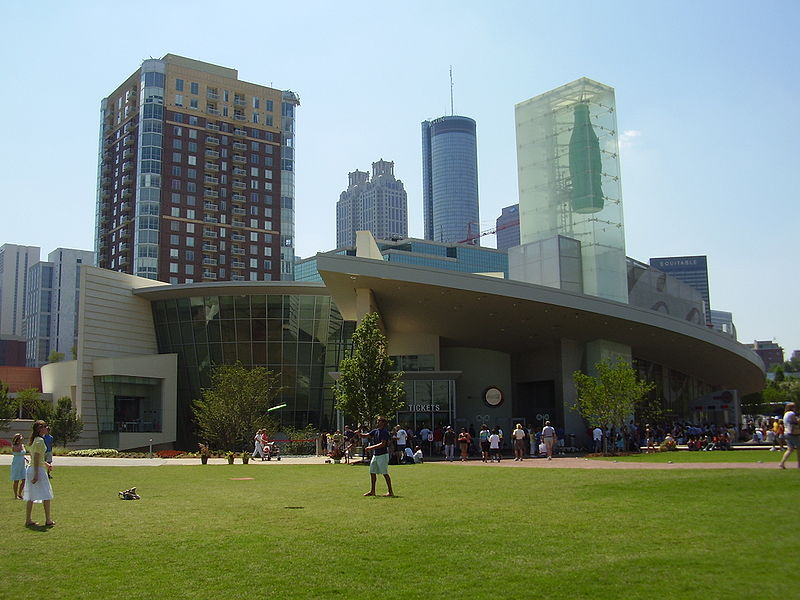
\includegraphics[height=100px]{content/day3/cocacola.jpg}

Tuesday, June 11, 2013, 7:00pm -- 9:00am \vspace{1em}\\
The World of Coca-Cola\\
121 Baker St. NW\\
Atlanta, GA 30313-1807\\
\end{center}

\noindent
This year's NAACL banquet promises to be a unique and interactive experience! Taking place in the intriguing World of Coca Cola Museum, attendees will have access to a multi-sensory 4D theater, an extraordinary 1880s soda fountain, the smallest bottling line in the world, plus an opportunity to sample nearly 70 different beverages from around the globe. Multiple buffet stations and seating areas will allow banquet-goers to enjoy the food and explore the museum at their leisure. And, of course there will be a DJ for your dancing pleasure. The banquet will take place at the World of Coca Cola Museum , Tuesday evening, June 11th. So, save yourselves the standard \$15-16 entrance fee and join us on Tuesday.


\newpage


\clearpage
%\section{Oral Presentations}
\noindent
\vspace{1em}\par\centerline{\bfseries\Large Paper Abstracts}\vspace{1em}\par
\addcontentsline{toc}{section}{Paper Abstracts}
\paperabstract{Tuesday}{10:45am--11:00am}{\Btitle}{\PBC}{main-047}
\paperabstract{Tuesday}{11:00am--11:15am}{\Btitle}{\PBC}{main-022}
\paperabstract{Tuesday}{11:15am--11:30am}{\Btitle}{\PBC}{main-444}
\paperabstract{Tuesday}{11:30am--11:45am}{\Btitle}{\PBC}{main-392}
\paperabstract{Tuesday}{11:45am--12:00pm}{\Btitle}{\PBC}{main-071}
\paperabstract{Tuesday}{10:45am--11:00am}{\Btitle}{\PLZBLRM}{main-016}
\paperabstract{Tuesday}{11:00am--11:15am}{\Btitle}{\PLZBLRM}{main-106}
\paperabstract{Tuesday}{11:15am--11:30am}{\Btitle}{\PLZBLRM}{main-400}
\paperabstract{Tuesday}{11:30am--11:45am}{\Btitle}{\PLZBLRM}{main-310}
\paperabstract{Tuesday}{11:45am--12:00pm}{\Btitle}{\PLZBLRM}{main-314}
\paperabstract{Tuesday}{10:45am--11:00am}{\Btitle}{\PDE}{main-329}
\paperabstract{Tuesday}{11:00am--11:15am}{\Btitle}{\PDE}{main-404}
\paperabstract{Tuesday}{11:15am--11:30am}{\Btitle}{\PDE}{main-455}
\paperabstract{Tuesday}{11:30am--11:45am}{\Btitle}{\PDE}{main-442}
\paperabstract{Tuesday}{11:45am--12:00pm}{\Btitle}{\PDE}{main-353}

\paperabstract{Tuesday}{2:00pm--2:15pm}{\Btitle}{\PBC}{main-001}
\paperabstract{Tuesday}{2:15pm--2:30pm}{\Btitle}{\PBC}{main-119}
\paperabstract{Tuesday}{2:30pm--2:45pm}{\Btitle}{\PBC}{main-037}
\paperabstract{Tuesday}{2:45pm--3:00pm}{\Btitle}{\PBC}{main-197}
\paperabstract{Tuesday}{3:00pm--3:15pm}{\Btitle}{\PBC}{main-434}
\paperabstract{Tuesday}{2:00pm--2:15pm}{\Btitle}{\PLZBLRM}{main-114}
\paperabstract{Tuesday}{2:15pm--2:30pm}{\Btitle}{\PLZBLRM}{main-046}
\paperabstract{Tuesday}{2:30pm--2:45pm}{\Btitle}{\PLZBLRM}{main-163}
\paperabstract{Tuesday}{2:45pm--3:00pm}{\Btitle}{\PLZBLRM}{main-417}
\paperabstract{Tuesday}{3:00pm--3:15pm}{\Btitle}{\PLZBLRM}{main-375}
\paperabstract{Tuesday}{2:00pm--2:15pm}{\Btitle}{\PDE}{main-292}
\paperabstract{Tuesday}{2:15pm--2:30pm}{\Btitle}{\PDE}{main-462}
\paperabstract{Tuesday}{2:30pm--2:45pm}{\Btitle}{\PDE}{main-098}
\paperabstract{Tuesday}{2:45pm--3:00pm}{\Btitle}{\PDE}{main-274}
\paperabstract{Tuesday}{3:00pm--3:15pm}{\Btitle}{\PDE}{main-160}

\clearpage{\thispagestyle{emptyheader}\cleardoublepage}

 
%\addcontentsline{toc}{chapter}{Program}
\setlength{\parindent}{0in}
\setlength{\parskip}{2ex}
\renewcommand{\baselinestretch}{0.87}

\begin{center}
{\Large \bf
  Conference Program Summary
}
\end{center}
\vspace{-10mm}
%\usepackage{graphicx}
\graphicspath{{./}{../templates/}{../templates/logo/}}
\includegraphics[height=1.1\textheight]{starsem-sts-semeval-schedule_summary_130510e1.pdf}
\newpage
\graphicspath{{./}{../templates/}{../templates/logo/}}
\includegraphics[height=1.1\textheight]{starsem-sts-semeval-schedule_summary_130510e2.pdf}
\newpage


\begin{center}
{\Large \bf
  Conference Program
}
\end{center}
\vspace{3mm}
\begin{tabular}{p{20mm}p{128mm}}
\multicolumn{2}{l}{\bf Day 1: Thursday June 13th 2013} \\
\\
 & {\bf (08:00--08:45) Registration} \\
\\
 & {\bf Session *SEM1: (08:45--10:30) Opening Remarks and *SEM Long Papers (1)} \\
\\
9:00--9:30 & \hyperlink{page.1}{\em Towards a Formal Distributional Semantics: Simulating Logical Calculi with Tensors}\\
         & Edward Grefenstette \\
\\

9:30--10:00 & \hyperlink{page.11}{\em Montague Meets Markov: Deep Semantics with Probabilistic Logical Form}\\
         & Islam Beltagy, Cuong Chau, Gemma Boleda, Dan Garrette, Katrin Erk and Raymond Mooney \\
\\

10:00--10:30 & \hyperlink{page.22}{\em Coarse to Fine Grained Sense Disambiguation in Wikipedia}\\
         & Hui Shen, Razvan Bunescu and Rada Mihalcea \\
\\

 & {\bf (10:30--11:00) Coffee Break} \\
\\
 & {\bf Session ST1: (11:00--12:30) STS Shared Task (1)} \\
\\
11:00--11:30 & \hyperlink{page.32}{\em *SEM 2013 shared task: Semantic Textual Similarity}\\
         & Eneko Agirre, Daniel Cer, Mona Diab, Aitor Gonzalez-Agirre and Weiwei Guo \\
\\

11:30--11:50 & \hyperlink{page.44}{\em UMBC\_EBIQUITY-CORE: Semantic Textual Similarity Systems}\\
         & Lushan Han, Abhay L. Kashyap, Tim Finin, James Mayfield and Jonathan Weese \\
\\

11:50--12:10 & \hyperlink{page.53}{\em iKernels-Core: Tree Kernel Learning for Textual Similarity}\\
         & Aliaksei Severyn, Massimo Nicosia and Alessandro Moschitti \\
\\

12:10--12:30 & \hyperlink{page.59}{\em UNITOR-CORE\_TYPED: Combining Text Similarity and Semantic Filters through SV Regression}\\
         & Danilo Croce, Valerio Storch and Roberto Basili \\
\\

\end{tabular}
\newpage
\begin{tabular}{p{20mm}p{138mm}}
\\
\multicolumn{2}{l}{\bf Day 1: Thursday June 13th 2013 (continued)} \\\\
 & {\bf (12:30--2:00) Lunch} \\
\\
 & {\bf Session ST2a: (2:00--2:40) STS Shared Task (2)} \\
\\
2:00--2:20 & \hyperlink{page.66}{\em NTNU-CORE: Combining strong features for semantic similarity}\\
         & Erwin Marsi, Hans Moen, Lars Bungum, Gleb Sizov, Bj\"{o}rn Gamb\"{a}ck and Andr\'{e} Lynum \\
\\

2:20--2:40 & \hyperlink{page.74}{\em SXUCFN-Core: STS Models Integrating FrameNet Parsing Information}\\
         & Sai Wang, Ru Li, Ruibo Wang, Zhiqiang Wang and Xia Zhang \\
\\

 & {\bf Session ST2b: (2:40--3:30) STS Poster boosters} \\
\\
 & {\bf (3:30--4:00) Coffee Break} \\
\\
 & {\bf Session *SEM2a: (4:00--4:25) *SEM Short Papers (1)} \\
\\
4:00--4:25 & \hyperlink{page.80}{\em Unsupervised Word Usage Similarity in Social Media Texts}\\
         & Spandana Gella, Paul Cook and Bo Han \\
\\

 & {\bf Session *SEM2b: (4:30--6:00) *SEM Panel: Toward Deep Natural Language Understanding: Kevin Knight (USC/ISI), Christopher Manning (Stanford University), Martha Palmer (University of Colorado, Boulder), Owen Rambow (Columbia University), Dan Roth (University of Illinois Urbana Champagne)} \\
\\
 & {\bf Session PLN1: (6:30--8:30) *SEM Opening Reception and STS Poster Session} \\
\\
 & \hyperlink{page.86}{\em UCAM-CORE: Incorporating structured distributional similarity into STS}\\
         & Tamara Polajnar, Laura Rimell and Douwe Kiela \\
\\

 & \hyperlink{page.91}{\em PolyUCOMP-CORE\_TYPED: Computing Semantic Textual Similarity using Overlapped Senses}\\
         & Jian Xu and Qin Lu \\
\\

 & \hyperlink{page.97}{\em HENRY-CORE: Domain Adaptation and Stacking for Text Similarity}\\
         & Michael Heilman and Nitin Madnani \\
\\

 & \hyperlink{page.104}{\em DeepPurple: Lexical, String and Affective Feature Fusion for Sentence-Level Semantic Similarity Estimation}\\
         & Nikolaos Malandrakis, Elias Iosif, Vassiliki Prokopi, Alexandros Potamianos and Shrikanth Narayanan \\
\\

 & \hyperlink{page.110}{\em UMCC\_DLSI: Textual Similarity based on Lexical-Semantic features}\\
         & Alexander Ch\'{a}vez, H\'{e}ctor D\'{a}vila, Yoan Guti\'{e}rrez, Armando Collazo, Jos\'{e} I. Abreu, Antonio Fern\'{a}ndez Orqu\'{i}n, Andr\'{e}s Montoyo and Rafael Mu\~{n}oz \\
\\

\end{tabular}
\newpage
\begin{tabular}{p{20mm}p{138mm}}
\\
\multicolumn{2}{l}{\bf Day 1: Thursday June 13th 2013 (continued)} \\\\
 & \hyperlink{page.120}{\em BUT-TYPED: Using domain knowledge for computing typed similarity}\\
         & Lubomir Otrusina and Pavel Smrz \\
\\

 & \hyperlink{page.125}{\em ECNUCS: Measuring Short Text Semantic Equivalence Using Multiple Similarity Measurements}\\
         & Zhu Tiantian and Man Lan \\
\\

 & \hyperlink{page.133}{\em UBC\_UOS-TYPED: Regression for typed-similarity}\\
         & Eneko Agirre, Nikolaos Aletras, Aitor Gonzalez-Agirre, German Rigau and Mark Stevenson \\
\\

 & \hyperlink{page.139}{\em KnCe2013-CORE:Semantic Text Similarity by use of Knowledge Bases}\\
         & Hermann Ziak and Roman Kern \\
\\

 & \hyperlink{page.144}{\em UPC-CORE: What Can Machine Translation Evaluation Metrics and Wikipedia Do for Estimating Semantic Textual Similarity?}\\
         & Alberto Barr\'{o}n-Cede\~{n}o, Llu\'{i}s M\`{a}rquez, Maria Fuentes, Horacio Rodriguez and Jordi Turmo \\
\\

 & \hyperlink{page.149}{\em MayoClinicNLP--CORE: Semantic representations for textual similarity}\\
         & Stephen Wu, Dongqing Zhu, Ben Carterette and Hongfang Liu \\
\\

 & \hyperlink{page.156}{\em SRIUBC-Core: Multiword Soft Similarity Models for Textual Similarity}\\
         & Eric Yeh \\
\\

 & \hyperlink{page.163}{\em LIPN-CORE: Semantic Text Similarity using n-grams, WordNet, Syntactic Analysis, ESA and Information Retrieval based Features}\\
         & Davide Buscaldi, Joseph Le Roux, Jorge J. Garcia Flores and Adrian Popescu \\
\\

 & \hyperlink{page.170}{\em UNIBA-CORE: Combining Strategies for Semantic Textual Similarity}\\
         & Annalina Caputo, Pierpaolo Basile and Giovanni Semeraro \\
\\

 & \hyperlink{page.177}{\em DLS$@$CU-CORE: A Simple Machine Learning Model of Semantic Textual Similarity}\\
         & Md. Sultan, Steven Bethard and Tamara Sumner \\
\\

 & \hyperlink{page.182}{\em KLUE-CORE: A regression model of semantic textual similarity}\\
         & Paul Greiner, Thomas Proisl, Stefan Evert and Besim Kabashi \\
\\

 & \hyperlink{page.188}{\em IBM\_EG-CORE: Comparing multiple Lexical and NE matching features in measuring Semantic Textual similarity}\\
         & Sara Noeman \\
\\

\end{tabular}
\newpage
\begin{tabular}{p{20mm}p{138mm}}
\\
\multicolumn{2}{l}{\bf Day 1: Thursday June 13th 2013 (continued)} \\\\
 & \hyperlink{page.195}{\em SOFTCARDINALIRY-CORE: Improving Text Overlap with Distributional Measures for Semantic Textual Similarity}\\
         & Sergio Jimenez, Claudia Becerra and Alexander Gelbukh \\
\\

 & \hyperlink{page.203}{\em CLaC-CORE: Exhaustive Feature Combination for Measuring Textual Similarity}\\
         & Ehsan Shareghi and Sabine Bergler \\
\\

 & \hyperlink{page.208}{\em UniMelb\_NLP-CORE: Integrating predictions from multiple domains and feature sets for estimating semantic textual similarity}\\
         & Spandana Gella, Bahar Salehi, Marco Lui, Karl Grieser, Paul Cook and Timothy Baldwin \\
\\

 & \hyperlink{page.217}{\em CFILT-CORE: Semantic Textual Similarity using Universal Networking Language}\\
         & Avishek Dan and Pushpak Bhattacharyya \\
\\

 & \hyperlink{page.222}{\em CPN-CORE: A Text Semantic Similarity System Infused with Opinion Knowledge}\\
         & Carmen Banea, Yoonjung Choi, Lingjia Deng, Samer Hassan, Michael Mohler, Bishan Yang, Claire Cardie, Rada Mihalcea and Jan Wiebe \\
\\

 & \hyperlink{page.230}{\em INAOE\_UPV-CORE: Extracting Word Associations from Document Corpora to estimate Semantic Textual Similarity}\\
         & Fernando S\'{a}nchez-Vega, Manuel Montes-y-G\'{o}mez, Paolo Rosso and Luis Villase\~{n}or-Pineda \\
\\

 & \hyperlink{page.235}{\em CNGL-CORE: Referential Translation Machines for Measuring Semantic Similarity}\\
         & Ergun Bicici and Josef Van Genabith \\
\\

\multicolumn{2}{l}{\bf Day 2: Friday June 14th 2013} \\
\\
 & {\bf (08:00--08:30) Registration} \\
\\
 & {\bf Session *SEM3: (08:30--09:30) *SEM Short Papers (2)} \\
\\
8:30--8:55 & \hyperlink{page.242}{\em A Dataset of Syntactic-Ngrams over Time from a Very Large Corpus of English Books}\\
         & Yoav Goldberg and Jon Orwant \\
\\

8:55--9:20 & \hyperlink{page.249}{\em Distinguishing Common and Proper Nouns}\\
         & Judita Preiss and Mark Stevenson \\
\\

9:20--9:30 & Short break for re-organization \\
\\
\end{tabular}
\newpage
\begin{tabular}{p{20mm}p{138mm}}
\\
\multicolumn{2}{l}{\bf Day 2: Friday June 14th 2013 (continued)} \\\\
 & {\bf Session PLN2: (09:30--10:30) Keynote address: David Forsyth (University of Illinois Urbana Champagne)} \\
\\
 & {\bf (10:30--11:00) Coffee Break} \\
\\
 & {\bf Session *SEM4: (11:00--12:30) *SEM Long Papers (2)} \\
\\
11:00--11:30 & \hyperlink{page.254}{\em Exploring Vector Space Models to Predict the Compositionality of German Noun-Noun Compounds}\\
         & Sabine Schulte im Walde, Stefan M\"{u}ller and Stefan Roller \\
\\

11:30--12:00 & \hyperlink{page.265}{\em Predicting the Compositionality of Multiword Expressions Using Translations in Multiple Languages}\\
         & Bahar Salehi and Paul Cook \\
\\

12:00--12:30 & \hyperlink{page.275}{\em Metaphor Identification as Interpretation}\\
         & Ekaterina Shutova \\
\\

 & {\bf (12:30--1:30) Lunch} \\
\\
 & {\bf Session PLN3: (1:30--2:30) *SEM / STS Shared Task / SemEval Panel} \\
\\
 & {\bf Session *SEM5: (2:30--3:30) *SEM Long Papers (3)} \\
\\
2:30--3:00 & \hyperlink{page.285}{\em Using the text to evaluate short answers for reading comprehension exercises}\\
         & Andrea Horbach, Alexis Palmer and Manfred Pinkal \\
\\

3:00--3:30 & \hyperlink{page.295}{\em Choosing the Right Words: Characterizing and Reducing Error of the Word Count Approach}\\
         & Hansen Andrew Schwartz, Johannes Eichstaedt, Eduardo Blanco, Lukasz Dziurzyński, Margaret L. Kern, Stephanie Ramones, Martin Seligman and Lyle Ungar \\
\\

\end{tabular}
\newpage
\begin{tabular}{p{20mm}p{138mm}}
\\
\multicolumn{2}{l}{\bf Day 2: Friday June 14th 2013 (continued)} \\\\
 & {\bf (3:30--4:00) Coffee Break} \\
\\
 & {\bf Session *SEM6: (4:00--5:30) *SEM Long Papers (4)} \\
\\
4:00--4:30 & \hyperlink{page.305}{\em Automatically Identifying Implicit Arguments to Improve Argument Linking and Coherence Modeling}\\
         & Michael Roth and Anette Frank \\
\\

4:30--5:00 & \hyperlink{page.316}{\em Bootstrapping Semantic Role Labelers from Parallel Data}\\
         & Mikhail Kozhevnikov and Ivan Titov \\
\\

5:00--5:30 & \hyperlink{page.327}{\em Semantic Parsing Freebase: Towards Open-domain Semantic Parsing}\\
         & Qingqing Cai and Alexander Yates \\
\\

 & {\bf Session *SEM7: (5:30--6:00) Best Papers Awards and Closing Remarks} \\
\\


\end{tabular}

% \chapter{Tutorials: Sunday, June 9}
\thispagestyle{emptyheader}
\setheaders{Tutorials}{Sunday, June 9, 2013}
\vspace{-3em}
\sloppy
%\addcontentsline{toc}{chapter}{Sunday, Jun 9, 2013: Tutorials}
\setlength{\parindent}{0in}
\setlength{\parskip}{2ex}
\renewcommand{\baselinestretch}{0.87}

\section*{Overview}

\begin{SingleTrackSchedule}
 7:30am & -- & 6:00pm &
 {\bfseries Registration} \hfill (\RegLoc)  \\
 \\

 9:00am & -- & 12:30pm &
 {\bfseries Morning Session} \\
 \\
 
 & & & 
 {\em Deep Learning for NLP (without Magic)}\hfill (\TutLocA)\newline
 Richard Socher and Christopher D. Manning \\
 \\

 & & &
 {\em Discourse Processing}\hfill (\TutLocB)\newline
 Manfred Stede \\
 \\

 & & &
 {\em NLP for uncertain data at scale}\hfill (\TutLocC)\newline
 Sameep Mehta and L V Subramaniam \\
 \\

 12:30pm & -- & 2:00pm &
 {\bf Lunch} \\
 \\

 1:00pm & -- & 6:00pm &
 {\bf NAACL Board Meeting}\hfill (\BRDRM) \newline
 \emph{(Lunch provided)} \\
 \\

 2:00pm & -- & 5:30pm &
 {\bfseries Afternoon Session} \\
 \\

 & & & 
 {\em Semantic Role Labeling}\hfill (\TutLocD)\newline
 Martha Palmer, Ivan Titov and Shumin Wu \\
 \\

 & & &  
 {\em Spectral Learning Algorithms for Natural Language}\hfill(\TutLocE)\newline
 {\em Processing}\newline
 Shay Cohen, Michael Collins, Dean Foster, Karl Stratos and Lyle Ungar \\
 \\

 & & & 
 {\em Morphological, Syntactical and Semantic Knowledge in}\hfill(\TutLocF)\newline
 {\em Statistical Machine Translation}\newline
 Marta Ruiz Costa-juss\`{a} and Chris Quirk \\
 \\

 6:00pm & -- & 9:00pm
 & {\bf Welcoming Reception}\hfill(\ATLBRM) \\

\end{SingleTrackSchedule}


\clearpage
\begin{bio}
\noindent
{\bfseries Richard Socher} is a PhD student at Stanford working with Chris Manning and Andrew Ng. His research interests are machine learning for NLP and vision. He is interested in developing new models that learn useful features, capture compositional and hierarchical structure in multiple modalities and perform well across different tasks. He was awarded the 2011 Yahoo! Key Scientific Challenges Award, the Distinguished Application Paper Award at ICML 2011 and a Microsoft Research PhD Fellowship in 2012.

\noindent
{\bfseries Christopher Manning} is an Associate Professor of Computer Science and Linguistics at Stanford University (PhD, Stanford, 1995). Manning has coauthored leading textbooks on statistical approaches to NLP (Manning and Schuetze 1999) and information retrieval (Manning et al. 2008). His recent work concentrates on machine learning and natural language processing, including applications such as statistical parsing and text understanding, joint probabilistic inference, clustering, and deep learning over text and images.
\end{bio}




\section%
    [\textbf{T1:} Deep Learning for NLP (without Magic) (R. Socher and M.~D. Manning)]
    {Tutorial 1}
\index{Socher, Richard}\label{TutA}
\index{Manning, Christopher~D.}
\begin{center}
\begin{Large}
\bfseries Deep Learning for NLP (without Magic)\\ \vspace{2em}\par
\end{Large}

{\itshape Richard Socher and Christopher D. Manning}\vspace{1em}\par
Sunday, June 9, 2013, 9:00am -- 12:30pm \vspace{1em}\\
\TutLocA
\end{center}

\noindent
{\bfseries Abstract:} Machine learning is everywhere in today's NLP, but by and large machine learning amounts to numerical optimization of weights for human designed representations and features. The goal of deep learning is to explore how computers can take advantage of data to develop features and representations appropriate for complex interpretation tasks. This tutorial aims to cover the basic motivation, ideas, models and learning algorithms in deep learning for natural language processing. Recently, these methods have been shown to perform very well on various NLP tasks such as language modeling, POS tagging, named entity recognition, sentiment analysis and paraphrase detection, among others. The most attractive quality of these techniques is that they can perform well without any external hand-designed resources or time-intensive feature engineering. Despite these advantages, many researchers in NLP are not familiar with these methods. Our focus is on insight and understanding, using graphical illustrations and simple, intuitive derivations. The goal of the tutorial is to make the inner workings of these techniques transparent, intuitive and their results interpretable, rather than black boxes labeled "magic here". The first part of the tutorial presents the basics of neural networks, neural word vectors, several simple models based on local windows and the math and algorithms of training via backpropagation. In this section applications include language modeling and POS tagging. In the second section we present recursive neural networks which can learn structured tree outputs as well as vector representations for phrases and sentences. We cover both equations as well as applications. We show how training can be achieved by a modified version of the backpropagation algorithm introduced before. These modifications allow the algorithm to work on tree structures. Applications include sentiment analysis and paraphrase detection. We also draw connections to recent work in semantic compositionality in vector spaces. The principle goal, again, is to make these methods appear intuitive and interpretable rather than mathematically confusing. By this point in the tutorial, the audience members should have a clear understanding of how to build a deep learning system for word-, sentence- and document-level tasks. The last part of the tutorial gives a general overview of the different applications of deep learning in NLP, including bag of words models. We will provide a discussion of NLP-oriented issues in modeling, interpretation, representational power, and optimization.
\clearpage
\begin{bio}
\noindent
{\bfseries Manfred Stede}, University of Potsdam. After completing his dissertation on the role of lexical semantics in multilingual text generation, Manfred Stede shifted his research focus towards problems of discourse structure and its role in various applications of text understanding. For discourse structure, his work centered on coherence relations and associated structural descriptions of text, and on the linguistic signals of such relations, especially connectives. From the early 2000s on, he developed the Potsdam Commentary Corpus as an example of (German) texts analyzed simultaneously on multiple levels, including sentential syntax, coreference, and rhetorical structure; in parallel, the technical infrastructure of a database for querying and visualizing multi-layer corpora was developed. In recent years, more analysis levels have been added to the corpus (e.g., content zones, connectives and their arguments). As for applications, Manfred worked on text summarization and various tasks of information extraction; more recently, his focus has been on issues of subjectivity and sentiment analysis.
\end{bio}

\section%
    [\textbf{T2:} Discourse Processing (M. Stede)]
    {Tutorial 2}
\index{Stede, M.}\label{TutV}
\begin{center}
\begin{Large}
\bfseries Discourse Processing\\ \vspace{2em}\par
\end{Large}

{\itshape Manfred Stede (University of Potsdam)}\vspace{1em}\par
Sunday, June 9, 2013, 9:00am -- 12:30pm \vspace{1em}\\
\TutLocB
\end{center}

\noindent
{\bfseries Abstract:} The observation that discourse is more than a mere sequence of utterances or sentences amounts to a truism. But what follows from this? In what way does the "value added" arise when segments of discourse are juxtaposed - how does hierarchical structure originate from a linearized discourse?

While many discourse phenomena apply to dialogue and monologue alike, this tutorial will center its attention on monologue written text. The perspective taken is that of practical language processing: We study methods for automatically deriving discourse information from text, and point to aspects of their implementation. The emphasis is on breadth rather than depth, so that the attendees will get an overview of the central tasks of discourse processing, with pointers to the literature for studying the individual problems in more depth. Much of the tutorial will follow the line of the recent book M. Stede: Discourse Processing. Morgan \& Claypool 2011.

Specifically, we will study the most important ways of ascribing structure to discourse. This is, first, a breakdown into functional units that are characteristic for the genre of the text. A news message, for example, is conventionally structured in a different way than a scientific paper is. For grasping this level of structure, the patterns that are characteristic for the specific genre need to be modeled.

Second, an ongoing text, unless it is very short, will cover different topics and address them in a sensible linear order. This is largely independent of genre, and since the notion of topic is relatively vague, it is harder to describe and sometimes difficult to identify. The common approach is to track the distribution of content words across the text, but in addition, overt signals for topic switches can be exploited.

Third, the identification of coreference links is a central aspect of discourse processing, and has received much attention in computational linguistics. We will survey the corpus-based methods that have dominated the field in recent years, and then look at the ramifications that the set of all coreference links in a text has for its structure.

Fourth, we investigate the structure resulting from establishing coherence relations (e.g., Cause, Contrast) among adjacent text segments. The term "discourse parsing" is often used for the task of identifying such relations (by exploiting more or less explicit linguistic signals) and building tree structures that reflect the semantic or pragmatic scaffolding of a (portion of) text.

Thus emerges a picture of a text as a series of different, yet related, layers of analysis. The final part of the tutorial addresses the issue of inter-connections between these levels. As a tool for accessing such multi-layered text corpora, we will see how the (open-source) ANNIS2 database allows for querying the data across different layers, and for visualizing different structural layers in appropriate ways.
\clearpage
\begin{bio}
\noindent
{\bfseries Sameep Mehta} is researcher in Information Management Group at IBM Research India. He received his M.S. and Ph.D. from The Ohio State University, USA in 2006. He also holds an Adjunct Faculty position at the International Institute of Information Technology, New Delhi. Sameep regularly advises MS and PhD students at University of Delhi and IIT Delhi. He regularly delivers Tutorials at COMAD (2009, 2010 and 2011). His current research interests include Data Mining, Business Analytics, Service Science, Text Mining, and Workforce Optimization.
\noindent

{\bfseries L Venkata Subramaniam} manages the information management analytics and solutions group at IBM Research India. He received his PhD from IIT Delhi in 1999. His research focuses on unstructured information management, statistical natural language processing, noisy text analytics, text and data mining, information theory, speech and image processing. He often teaches and guides student thesis at IIT Delhi on these topics. His tutorial titled Noisy Text Analytics was the second largest at NAACL-HLT 2010. He co founded the AND (Analytics for Noisy Unstructured Text Data) workshop series and also co-chaired the first four workshops, 2007-2010. He was guest co-editor of two special issues on Noisy Text Analytics in the International Journal of Document Analysis and Recognition in 2007 and 2009.
\end{bio}


\section%
    [\textbf{T3:} Towards Reliability-Aware Entity Analytics and Integration for Noisy Text at Scale (S. Mehta and L.~V. Subramaniam)]
    {Tutorial 3}
\index{Mehta, Sameep}\label{TutC}
\index{Subramaniam, L.~Venkata.}
\begin{center}
\begin{Large}
\bfseries Towards Reliability-Aware Entity Analytics and Integration for Noisy Text at Scale\\ \vspace{2em}\par
\end{Large}

{\itshape Sameep Mehta and L.~Venkata Subramaniam}\vspace{1em}\par
Sunday, June 9, 2013, 9:00am -- 12:30pm \vspace{1em}\\
\TutLocC
\end{center}

\noindent
{\bfseries Abstract:} Due to easy to use apps (Facebook, Twitter, etc.), higher Internet connectivity and always on facility allowed by smart phones, the key characteristics of raw data are changing. This new data can be characterized by 4V's - Volume, Velocity, Variety and Veracity. For example during a Football match, some people will Tweet about goals, penalties, etc., while others may write longer blogs and further there will be match reports filed in trusted online news media after the match. Although the sources may be varied, the data describes and provides multiple evidences for the same event. Such multiple evidences should be used to strengthen the belief in the underlying physical event as the individual data points may have inherent uncertainty. The uncertainty can arise from inconsistent, incomplete and ambiguous reports. The uncertainty is also because the trust levels of the different sources vary and affect the overall reliability. We will summarize various efforts to perform reliability aware entity integration.

The other problem in text analysis in such setting is posed by presence of noise in the text. Since the text is produced in several informal settings such as email, blogs, tweet, SMS, chat and is inherently noisy and has several veracity issues. For example, missing punctuation and the use of non-standard words can often hinder standard natural language processing techniques such as part-of-speech tagging and parsing. Further downstream applications such as entity extraction, entity resolution and entity completion have to explicitly handle noise in order to return useful results. Often, depending on the application, noise can be modeled and it may be possible to develop specific strategies to immunize the system from the effects of noise and improve performance. Also the aspect of reliability is key as a lot of this data is ambiguous, incomplete, conflicting, untrustworthy and deceptive. The key goals of this tutorial are:

\begin{itemize}
\item Draw the attention of researchers towards methods for doing entity analytics and integration on data with 4V characteristics.
\item Differentiate between noise and uncertainty in such data.
\item Provide an in-depth discussion on handling noise in NLP based methods.
\item Finally, handling uncertainty through information fusion and integration.
\end{itemize}

This tutorial builds on two earlier tutorials — NAACL 2010 tutorial on Noisy Text and COMAD 2012 tutorial on Reliability Aware Data Fusion. In parallel the authors are also hosting a workshop on related topic "Reliability Aware Data Fusion" at SIAM Data Mining Conference, 2013.
\clearpage
\begin{bio}
\setlength{\parskip}{1ex}

\noindent
{\bfseries Martha Palmer} is a Professor of Linguistics and Computer Science, and a Fellow of the Institute of Cognitive Science at the University of Colorado. Her current research is aimed at building domain-independent and language independent techniques for semantic interpretation based on linguistically annotated data, such as Proposition Banks. She has been the PI on NSF, NIH and DARPA projects for linguistic annotation (syntax, semantics and pragmatics) of English, Chinese, Korean, Arabic and Hindi. She has been a member of the Advisory Committee for the DARPA TIDES program, Chair of SIGLEX, Chair of SIGHAN, a past President of the Association for Computational Linguistics, and is a Co-Editor of JNLE and of LiLT and is on the CL Editorial Board. She received her Ph.D. in Artificial Intelligence from the University of Edinburgh in 1985.

\noindent
{\bfseries Ivan Titov} joined the Saarland University as a junior faculty and head of a research group in November 2009, following a postdoc at the University of Illinois at Urbana-Champaign. He received his Ph.D. in Computer Science from the University of Geneva in 2008 and his master's degree in Applied Mathematics and Informatics from the St. Petersburg State Polytechnic University (Russia) in 2003. His research interests are in statistical natural language processing (models of syntax, semantics and sentiment) and machine learning (structured prediction methods, latent variable models, Bayesian methods).

\noindent
{\bfseries Shumin Wu} is a Computer Science PhD student (advised by Dr. Martha Palmer) at the University of Colorado. His current research is aimed at developing and applying semantic mapping (aligning and jointly inferring predicate-argument structures between languages) to Chinese dropped-pronoun recovery/alignment, automatic verb class induction, and other applications relevant to machine translation.
\end{bio}

\section%
    [\textbf{T4:} Semantic Role Labeling (M. Palmer, I. Titov and S. Wu)]
    {Tutorial 4}
\index{Palmer, Martha}\label{TutD}
\index{Titov, Ivan}
\index{Wu, Shumin}
\begin{center}
\begin{Large}
\bfseries Semantic Role Labeling\\ \vspace{2em}\par
\end{Large}

{\itshape Martha Palmer (University of Colorado), Ivan Titov (Saarland University), and Shumin Wu (University of Colorado)}\vspace{1em}\par
Sunday, June 9, 2013, 2:00pm -- 5:30pm \vspace{1em}\\
\TutLocD
\end{center}

\noindent
This tutorial will describe semantic role labeling, the assignment of semantic roles to eventuality participants in an attempt to approximate a semantic representation of an utterance. The linguistic background and motivation for the definition of semantic roles will be presented, as well as the basic approach to semantic role annotation of large amounts of corpora. Recent extensions to this approach that encompass light verb constructions and predicative adjectives will be included, with reference to their impact on English, Arabic, Hindi and Chinese. Current proposed extensions such as Abstract Meaning Representations and richer event representations will also be touched on.

Details of machine learning approaches will be provided, beginning with fully supervised approaches that use the annotated corpora as training material. The importance of syntactic parse information and the contributions of different feature choices, including tree kernels, will be discussed, as well as the advantages and disadvantages of particular machine learning algorithms and approaches such as joint inference. Appropriate considerations for evaluation will be presented as well as successful uses of semantic role labeling in NLP applications.

We will also cover techniques for exploiting unlabeled corpora and transferring models across languages. These include methods, which project annotations across languages using parallel data, induce representations solely from unlabeled corpora (unsupervised methods) or exploit a combination of a small amount of human annotation and a large unlabeled corpus (semi-supervised techniques). We will discuss methods based on different machine learning paradigms, including generative Bayesian models, graph-based algorithms and bootstrapping style techniques.
\clearpage
\begin{bio}
\noindent

\end{bio}

\section%
    [\textbf{T5:}  Spectral Learning Algorithms for Natural Language Processing (S. Cohen, M. Collins, D.~P. Foster, K. Stratos and L. Ungar)]
    {Tutorial 5}
\index{Cohen, Shay}\label{TutE}
\index{Collins, Michael}
\index{Foster, Dean P.}
\index{Stratos, Karl}
\index{Collins, Michael}
\index{Ungar, Lyle				}
\begin{center}
\begin{Large}
\bfseries Towards Reliability-Aware Entity Analytics and Integration for Noisy Text at Scale\\ \vspace{2em}\par
\end{Large}

{\itshape Shay Cohen (Columbia University), Michael Collins (Columbia University), Dean P. Foster (University of Pennsylvania), Karl Stratos (Columbia University), and Lyle Ungar (University of Pennsylvania)}\vspace{1em}\par
Sunday, June 9, 2013, 2:00am -- 5:30pm \vspace{1em}\\
\TutLocE
\end{center}

\noindent
{\bfseries Abstract:} Recent work in machine learning and NLP has developed spectral algorithms for many learning tasks involving latent variables. Spectral algorithms rely on singular value decomposition as a basic operation, usually followed by some simple estimation method based on the method of moments. From a theoretical point of view, these methods are appealing in that they offer consistent estimators (and PAC-style guarantees of sample complexity) for several important latent-variable models. This is in contrast to the EM algorithm, which is an extremely successful approach, but which only has guarantees of reaching a local maximum of the likelihood function.

From a practical point of view, the methods (unlike EM) have no need for careful initialization, and have recently been shown to be highly efficient (as one example, in work under submission by the authors on learning of latent-variable PCFGs, a spectral algorithm performs at identical accuracy to EM, but is around 20 times faster).

In this tutorial we will aim to give a broad overview of spectral methods, describing theoretical guarantees, as well as practical issues. We will start by covering the basics of singular value decomposition and describe efficient methods for doing singular value decomposition. The SVD operation is at the core of most spectral algorithms that have been developed.

We will then continue to cover canonical correlation analysis (CCA). CCA is an early method from statistics for dimensionality reduction. With CCA, two or more views of the data are created, and they are all projected into a lower dimensional space which maximizes the correlation between the views. We will review the basic algorithms underlying CCA, give some formal results giving guarantees for latent-variable models and also describe how they have been applied recently to learning lexical representations from large quantities of unlabeled data. This idea of learning lexical representations can be extended further, where unlabeled data is used to learn underlying representations which are subsequently used as additional information for supervised training.

We will also cover how spectral algorithms can be used for structured prediction problems with sequences and parse trees. A striking recent result by Hsu, Kakade and Zhang (2009) shows that HMMs can be learned efficiently using a spectral algorithm. HMMs are widely used in NLP and speech, and previous algorithms (typically based on EM) were guaranteed to only reach a local maximum of the likelihood function, so this is a crucial result. We will review the basic mechanics of the HMM learning algorithm, describe its formal guarantees, and also cover practical issues.

Last, we will cover work about spectral algorithms in the context of natural language parsing. We will show how spectral algorithms can be used to estimate the parameter models of latent-variable PCFGs, a model which serves as the base for state-of-the-art parsing models such as the one of Petrov et al. (2007). We will show what are the practical steps that are needed to be taken in order to make spectral algorithms for L-PCFGs (or other models in general) practical and comparable to state of the art.
\clearpage
\begin{bio}
\noindent
{\bfseries Marta R. Costa-jussà}, Institute for Infocomm Research (I2R), is a Telecommunication's Engineer by the Universitat Politècnica de Catalunya (UPC, Barcelona) and she received her PhD from the UPC in 2008. Her research experience is mainly in Automatic Speech Recognition, Machine Translation and Information Retrieval. She has worked at LIMSI-CNRS (Paris), Barcelona Media Innovation Center (Barcelona) and the Universidade de Sao Paulo (São Paulo). Since December 2012 she is working at Institute for Infocomm Research (Singapore) implementing the IMTraP project ("Integration of Machine Translation Paradigms") on Hybrid Machine Translation, funded by the European Marie Curie International Outgoing European Fellowship program. She is currently organizing the ACL Workshop HyTRA 2013 and she will be teaching a summer school course on hybrid machine translation at ESSLLI 2013.

\noindent
{\bfseries Chris Quirk}, Microsoft Research. After studying Computer Science and Mathematics at Carnegie Mellon University, Chris joined Microsoft in 2000 to work on the Intentional Programming project, an extensible compiler and development framework. He moved to the Natural Language Processing group in 2001, where his research has mostly focused on statistical machine translation powering Microsoft Translator, especially on several generations of a syntax directed translation system that powers over half of the translation systems. He is also interested in semantic parsing, paraphrase methods, and very practical problems such as spelling correction and transliteration.
\end{bio}

\section%
    [\textbf{T6:} Morphological, Syntactical and Semantic Knowledge in Statistical Machine Translation (M.~R. Costa-juss\`{a} and C. Quirk)]
    {Tutorial 6}
\index{Costa-juss\`{a}, Marta R.}\label{TutF}
\index{Titov, Ivan}
\index{Quirk, Chris}
\begin{center}
\begin{Large}
\bfseries Morphological, Syntactical and Semantic Knowledge in Statistical Machine Translation\\ \vspace{2em}\par
\end{Large}

{\itshape Marta R. Costa-juss\`{a} (Institute for Infocomm Research) and Chris Quirk (Microsoft Research)}\vspace{1em}\par
Sunday, June 9, 2013, 2:00am -- 5:30pm \vspace{1em}\\
\TutLocF
\end{center}

\noindent
{\bfseries Abstract:} 

This tutorial focuses on how morphology, syntax and semantics may be introduced into a standard phrase-based statistical machine translation system with techniques such as machine learning, parsing and word sense disambiguation, among others.

Regarding the phrase-based system, we will describe only the key theory behind it. The main challenges of this approach are that the output contains unknown words, wrong word orders and non-adequate translated words. To solve these challenges, recent research enhances the standard system using morphology, syntax and semantics.

Morphologically-rich languages have many different surface forms, even though the stem of a word may be the same. This leads to rapid vocabulary growth, as various prefixes and suffixes can combine with stems in a large number of possible combinations. Language model probability estimation is less robust because many more word forms occur rarely in the data. This morphologically-induced sparsity can be reduced by incorporating morphological information into the SMT system. We will describe the three most common solutions to face morphology: preprocessing the data so that the input language more closely resembles the output language; using additional language models that introduce morphological information; and post-processing the output to add proper inflections.

Syntax differences between the source and target language may lead to significant differences in the relative word order of translated words. Standard phrase-based SMT systems surmount reordering/syntactic challenges by learning from data. Most approaches model reordering inside translation units and using statistical methodologies, which limits the performance in language pairs with different grammatical structures. We will briefly introduce some recent advances in SMT that use modeling approaches based on principles more powerful flat phrases and better suited to the hierarchical structures of language: SMT decoding with stochastic synchronous context free grammars and syntax-driven translation models.

Finally, semantics are not directly included in the SMT core algorithm, which means that challenges such as polysemy or synonymy are either learned directly from data or they are incorrectly translated. We will focus on recent attempts to introduce semantics into statistical-based systems by using source context information.

The course material will be suitable both for attendees with limited knowledge of the field, and for researchers already familiar with SMT who wish to learn about modern tendencies in hybrid SMT. The mathematical content of the course include probability and simple machine learning, so reasonable knowledge of statistics and mathematics is required. There will be a small amount of linguistics and ideas from natural language processing.




% \chapter{Monday, June 10, 2013: Main Conference}
\thispagestyle{emptyheader}
\setheaders{NAACL HLT: Main Conference}{Monday, June 10, 2013}

\centerline{\bfseries\Large Overview}
\renewcommand{\arraystretch}{1.2}
\begin{SingleTrackSchedule}
  8:45am & -- &  9:00am & 
  \bfseries Welcome to NAACL 2013! \hfill (\ATLBRM)
  \\

  9:00am & -- & 10:10am & 
  \bfseries Invited talk by Gina Kuperberg -- Predicting Meaning: What the Brain tells us about the Architecture of Language Comprehension
  \\[1ex]%\hline[-2ex]

  10:10am & -- & 10:40am & \bfseries Break
  \\[1ex]%\hline[-2ex]

  10:40am & -- & 12:20pm & 
  \bfseries Parallel Sessions\hfill (\MOaLoc, \MObLoc, \MOcLoc)
  \\[1ex]%\hline[-2ex]
  
  12:20pm & -- & 2:00pm & 
  \bfseries Lunch\hfill (\StudLunchLoc)\newline
  \\[1ex]%\hline[-2ex]

  2:00am & -- & 3:40pm & 
  \bfseries Parallel Sessions\hfill (\MOaLoc, \MObLoc, \MOcLoc)
  \\[1ex]%\hline[-2ex]

  3:40am & -- & 4:10am & \bfseries Break
  \\[1ex]%\hline[-2ex]

  4:10pm & -- & 6:00pm & 
  \bfseries Poster Madness! \hfill (\PosterSessionLoc)
  \\[1ex]%\hline[-2ex]

  6:00am & -- & 6:30am & \bfseries Break
  \\[1ex]%\hline[-2ex]

  6:30pm & -- & 9:00pm & 
  \bfseries Posters \& Demonstrations
  \mbox{}~\hfill (200 Building Grand Atrium)
  \\[1ex]%\hline[-2ex]


\end{SingleTrackSchedule}
\newpage
%% \begin{landscape}
\vfill

\centerline{\bfseries\Large Schedule}%\vspace{-1ex}
%\section{Schedule}
\noindent
\begin{ThreeTrackSchedule}
\hline\BreakTime{7:30am}{5:00pm}{3}{Registration (\FOY)}\\\hline\noalign{\bigskip}
%\multicolumn{6}{c}{\ }\\[.25ex]
\hline
\BreakTime   {7:30am}{9:00am}{3}{Breakfast (\FOY)}\\\hline
\PlenaryEvent{9:00am}{9:15am}{3}{Welcome (\PLN)}\\\hline
\PlenaryEvent{9:15am}{10:30am}{3}{{\bfseries Invited Talk (\PLN)\linebreak
{\itshape Eduard Hovy:}  {``A New Semantics: Merging Propositional and Distributional Information''}}\linebreak
{\small\normalfont {\bfseries Chair:} {\itshape Ellen Riloff}}}\\\hline
\BreakTime{10:30am}{11:00am}{3}{Coffee Break (\FOY)}\\\hline

\multicolumn{3}{|c|}{\bfseries Parallel Sessions}
& \bfseries East Ballroom
& \bfseries West Ballroom
& \bfseries Drummond
\\\hline

&&
& \bfseries \DDP~I 
& \bfseries \MT~I 
& \bfseries \IE 
\\
&&
& {\small {\bfseries Chair:} {\itshape David Traum}} 
& {\small {\bfseries Chair:} {\itshape Daniel Marcu}} 
& {\small {\bfseries Chair:} {\itshape Radu Florian}} 
\\\hline


10:40am & -- & 11:05am & \paperentry{main-268}\\\hline
11:05am & -- & 11:30am & \paperentry{main-319}\\\hline
11:30am & -- & 11:55am & \paperentry{main-276}\\\hline
11:55am & -- & 12:20pm & \paperentry{main-419}\\\hline
10:40am & -- & 11:05am & \paperentry{main-441}\\\hline
11:05am & -- & 11:30am & \paperentry{main-282}\\\hline
11:30am & -- & 11:55am & \paperentry{main-174}\\\hline
11:55am & -- & 12:20pm & \paperentry{main-125}\\\hline
10:40am & -- & 11:05am & \paperentry{main-377}\\\hline
11:05am & -- & 11:30am & \paperentry{main-474}\\\hline
11:30am & -- & 11:55am & \paperentry{main-082}\\\hline
11:55am & -- & 12:20pm & \paperentry{main-370}\\\hline


\BreakTime{12:30pm}{1:15pm}{3}{Student Lunch (students only!; \StudLunchLoc)}\\\hline

\end{ThreeTrackSchedule}

\newpage

\begin{ThreeTrackSchedule}
\hline

\PlenaryEvent{1:15pm}{2:15pm}{3}{%
{\bfseries Student Research Workshop Panel:} ``{Reviewing Practices}''\linebreak
(open to all; \SRWPanelLoc)}\\\hline

\multicolumn{3}{|c|}{\bfseries Parallel Sessions}
& \bfseries East Ballroom
& \bfseries West Ballroom
& \bfseries Drummond
\\\hline

\bfseries 2:30pm & -- & \bfseries 4:00pm
& \bfseries \SLP  
& \bfseries \ML~I 
& \bfseries \LRE  \\
&&
& {\small {\bfseries Chair:} {\itshape Giuseppe Riccardi}} 
& {\small {\bfseries Chair:} {\itshape Hal Daum\'{e} III}} 
& {\small {\bfseries Chair:} {\itshape Jill Burstein}} 
\\\hline

2:00pm & -- & 2:25pm & \paperentry{main-233} & \paperentry{main-363}\\\hline
2:25pm & -- & 2:50pm & \paperentry{main-002} & \paperentry{main-429}\\\hline
2:50pm & -- & 3:15pm & \paperentry{main-239} & \paperentry{main-438}\\\hline
3:15pm & -- & 3:40pm & \paperentry{main-001} & \paperentry{main-361}\\\hline
2:00pm & -- & 2:25pm & \paperentry{main-266} & \paperentry{main-000}\\\hline
2:25pm & -- & 2:50pm & \paperentry{main-317}\\\hline
2:50pm & -- & 3:15pm & \paperentry{main-308}\\\hline
3:15pm & -- & 3:40pm & \paperentry{main-155}\\\hline


\BreakTime{4:00pm}{4:30pm}{3}{Coffee Break (\FOY)}\\\hline

\PlenaryEvent{4:30pm}{5:30pm}{3}{%
{\bfseries ---~\CBR~---\linebreak 
Posters and Demos: One-minute Madness (Poster Descriptions)} \linebreak
{\small {\bfseries Chair:} \textnormal{\itshape Joel Tetreault}} } \\\hline

\PlenaryEvent{6:00pm}{9:00pm}{3}{%
{\bfseries ---~\WBR~---\linebreak Poster Session and Demos (with Buffet Dinner)}}\\\hline

\end{ThreeTrackSchedule}
\end{landscape}
\newpage
%\thispagestyle{myheadings}
\section{Invited Talk: Gina R Kuperberg}
\index{Kuperberg, Gina R}
\begin{center}
%% --- Keynote Address ---
%% \vspace{2em}\\
%% \vfill

\begin{Large}
{\bfseries\Large ``Predicting Meaning: What the Brain tells us about the Architecture of Language Comprehension''}\vspace{1em}\par
\end{Large}

{\itshape Gina R. Kuperberg}\vspace{1em}\par
Monday, June 10, 2013, 9:00am -- 10:10am \vspace{1em}\\
\index{Kuperberg, Gina R.}
\PlenaryLoc \\
\vspace{1em}\par 
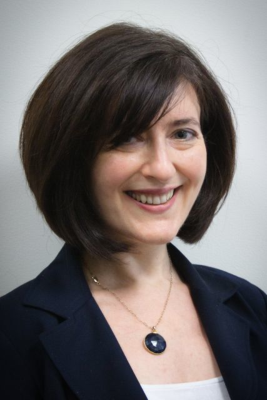
\includegraphics[height=100px]{content/day2/kuperberg-headshot.pdf}
\end{center}

\noindent
{\bfseries Abstract:} It is well established that we draw upon our real-world knowledge to predict
upcoming events and even individual words. I will discuss evidence that the neurocognitive
mechanisms that we engage in retrieving conceptual information associated with incoming words are
quite distinct from those engaged when these predictions are disconfirmed by the input. Drawing
broad links with computational models conceptualizing language comprehension as an incremental
process of belief updating, I will suggest that the engagement of these distinct neurocognitive
systems allows for comprehension that is both highly efficient and highly flexible (1).

I will first discuss studies using event-related potentials (ERPs) to examine online brain activity
during sentence and discourse comprehension. I will then draw some (still tentative) links between
this ERP literature and some relevant fMRI and MEG studies. Finally, I will discuss the advantages
of a predictive comprehension system. Predicting correctly clearly offers advantages in terms of
computational efficiency. Here I will argue that the costs incurred when we predict incorrectly are
also crucial for successful and flexible comprehension. Neurocognitive responses triggered by
prediction errors may rescue us from interpretation errors in noisy environments, may allow us learn
novel events, and may enable us to flexibly adjust our comprehension strategies in response to
everchanging task and environmental demands.

\vspace{3em}\par 

\vfill
\noindent
{\bfseries Biography}: Gina R Kuperberg is a Cognitive Neuroscientist and a Professor in the
Department of Psychology and the Cognitive Science Center at Tufts University, Boston. She is also a
Board Certified Psychiatrist and a Principal Investigator in the Psychiatry Neuroscience Program at
Massachusetts General Hospital, Harvard Medical School. Her research program aims to understand the
neurocognitive mechanisms by which the human brain builds meaning from language, and how these
mechanisms break down in neuropsychiatric disorders, particularly schizophrenia.

Dr.\ Kuperberg's Lab is situated across in both the Department of Psychology at Tufts and the
Martinos Center for Biomedical Imaging at Massachusetts General Hospital. The Lab uses multimodal
neuroimaging methods –– event-related potentials (ERPs), functional MRI (fMRI) and
magneto-encephalography (MEG) –– to probe both the spatial and temporal dimensions of cognition in
the brain. Her research program is funded by an RO1 from the National Institute of Mental Health
(NIMH), as well as awards from the Brain and Behavior Research Foundation and the Sidney Baer
Trust. She, her students, postdocs and collaborators publish in a wide range of journals of
Cognitive Neuroscience, Psycholinguistics, Experimental Psychology, Neuroimaging and Psychiatry.

Dr.\ Kuperberg has served as a standing member for the Language and Communication Study Section for
the National Institute of Health, and as a committee representative for Language for the Cognitive
Neuroscience society. Her research accomplishments have been recognized by several awards, including
the A.E. Bennett Research Award from the Society for Biological Psychiatry, the Joseph Zubin Award
for Significant Contributions to Research in Psychopathology, and an Award from Brain Research for
their most highly cited article, for her review of the architecture of the language system, Neural
Mechanisms of Language Comprehension: Challenges to Syntax.

Dr.\ Kuperberg earned her MD at St. Bartholomew's Medical School, London, and her PhD in Psychology
and Cognitive Neuroscience at Kings College, University of London. She completed an internship at
St. Bartholomew's Hospital and residency training in Psychiatry at the Maudsley Hospital and
Institute of Psychiatry, London. In 1998, she came to Boston where she completed research
fellowships in Neuroimaging and Cognitive Electrophysiology at Massachusetts General Hospital,
Harvard Medical School and Tufts University, working with David Caplan, Anders Dale and Phil
Holcomb.
\newpage
\newpage

%\section{Oral Presentations}
%\vspace{1em}\par\centerline{\bfseries\Large Paper Abstracts}\vspace{1em}\par
%% \addcontentsline{toc}{section}{Session 1}
\clearpage
\par\centerline{\bfseries\large Session M1a: Machine Translation}\vspace{1em}\par
\paperabstract{Monday}{10:40am--11:05am}{garbage}{garbage}{main-268}
\paperabstract{Monday}{11:05am--11:30am}{garbage}{garbage}{main-319}
\paperabstract{Monday}{11:30am--11:55am}{garbage}{garbage}{main-276}
\paperabstract{Monday}{11:55am--12:20pm}{garbage}{garbage}{main-419}
\clearpage
\par\centerline{\bfseries\large Session M1b: Information Extraction}\vspace{1em}\par
\paperabstract{Monday}{10:40am--11:05am}{garbage}{garbage}{main-441}
\paperabstract{Monday}{11:05am--11:30am}{garbage}{garbage}{main-282}
\paperabstract{Monday}{11:30am--11:55am}{garbage}{garbage}{main-174}
\paperabstract{Monday}{11:55am--12:20pm}{garbage}{garbage}{main-125}
\clearpage
\par\centerline{\bfseries\large Session M1c: Cognitive and Psycholinguistics}\vspace{1em}\par
\paperabstract{Monday}{10:40am--11:05am}{garbage}{garbage}{main-377}
\paperabstract{Monday}{11:05am--11:30am}{garbage}{garbage}{main-474}
\paperabstract{Monday}{11:30am--11:55am}{garbage}{garbage}{main-082}
\paperabstract{Monday}{11:55am--12:20pm}{garbage}{garbage}{main-370}
\clearpage
\par\centerline{\bfseries\large Session M2a: Parsing and Syntax}\vspace{1em}\par
\paperabstract{Monday}{2:00pm--2:25pm}{garbage}{garbage}{main-233}
\paperabstract{Monday}{2:25pm--2:50pm}{garbage}{garbage}{main-002}
\paperabstract{Monday}{2:50pm--3:15pm}{garbage}{garbage}{main-239}
\paperabstract{Monday}{3:15pm--3:40pm}{garbage}{garbage}{TACL-001}
\clearpage
\par\centerline{\bfseries\large Session M2b: Topic Modeling and Text Mining}\vspace{1em}\par
\paperabstract{Monday}{2:00pm--2:25pm}{garbage}{garbage}{main-266}
\paperabstract{Monday}{2:25pm--2:50pm}{garbage}{garbage}{main-317}
\paperabstract{Monday}{2:50pm--3:15pm}{garbage}{garbage}{main-308}
\paperabstract{Monday}{3:15pm--3:40pm}{garbage}{garbage}{main-155}
\clearpage
\par\centerline{\bfseries\large Session M2c: Spoken Language Processing}\vspace{1em}\par
\paperabstract{Monday}{2:00pm--2:25pm}{garbage}{garbage}{main-363}
\paperabstract{Monday}{2:25pm--2:50pm}{garbage}{garbage}{main-429}
\paperabstract{Monday}{2:50pm--3:15pm}{garbage}{garbage}{main-438}
\paperabstract{Monday}{3:15pm--3:40pm}{garbage}{garbage}{main-361}

\newpage

% I'm bypassing the \section command here because I didn't like the layout
% from the ACL-IJNLP handbook that I started from. UG

\setheaders{NAACL HLT: Poster and Demonstrations Session}{Monday, June 10, 2013}

\vspace{1em}\par\centerline{\bfseries\Large Poster Madness!}\vspace{1em}\par
\addcontentsline{toc}{section}{Poster madness!}

Prior to the poster session, poster presenters are given one minute each to pitch their
paper. Posters from the Student Research Workshop are included. Following the Poster Madness!
session, there will be a buffet dinner and a combined Posters and Demonstrations session.

\noindent
\vspace{1em}\par\centerline{\bfseries\large Main Conference Posters}\vspace{1em}\par
\posterabstract{main-180}
\posterabstract{main-393}
\posterabstract{main-345}
\posterabstract{main-108}
\posterabstract{main-195}
\posterabstract{main-410}
\posterabstract{main-020}
\posterabstract{main-206}
\posterabstract{main-089}
\posterabstract{main-420}
\posterabstract{TACL-002}
\posterabstract{main-289}
\posterabstract{main-184}
\posterabstract{main-293}
\posterabstract{main-120}
\posterabstract{main-390}
\posterabstract{main-431}
\posterabstract{main-137}
\posterabstract{main-457}
\posterabstract{main-336}
\posterabstract{main-402}
\posterabstract{main-075}
\posterabstract{main-385}
\posterabstract{main-300}
\posterabstract{main-128}
\posterabstract{main-264}
\posterabstract{main-278}
\posterabstract{main-397}
\posterabstract{main-212}
\posterabstract{main-250}
\posterabstract{main-313}
\posterabstract{main-351}
\posterabstract{main-225}
\posterabstract{main-340}
\posterabstract{main-023}
\posterabstract{main-446}
\posterabstract{main-004}
\posterabstract{main-372}
\posterabstract{main-066}
\posterabstract{main-449}
\posterabstract{main-095}
\posterabstract{main-057}
\posterabstract{main-283}
\posterabstract{main-275}
\posterabstract{main-467}
\posterabstract{main-070}
\posterabstract{main-221}
\posterabstract{main-072}


\noindent
\vspace{1em}\par\centerline{\bfseries\large Student Research Workshop Posters}\vspace{1em}\par
\noindent
%% \posterentry{srw-005}\\[1ex]
\posterentry{srw-020}\\[1ex]
\posterentry{srw-008}\\[1ex]
\posterentry{srw-007}\\[1ex]
\posterentry{srw-002}\\[1ex]
\posterentry{srw-010}\\[1ex]
\posterentry{srw-018}\\[1ex]
\posterentry{srw-015}\\[1ex]
\posterentry{srw-024}\\[1ex]
\posterentry{srw-016}\\[1ex]
\posterentry{srw-014}\\[1ex]
\posterentry{srw-012}\\[1ex]
\posterentry{srw-021}\\[1ex]

\posterabstract{srw-002}\par
\posterabstract{srw-005}\par
\posterabstract{srw-007}\par
\posterabstract{srw-008}\par
\posterabstract{srw-010}\par
\posterabstract{srw-012}\par
\posterabstract{srw-014}\par
\posterabstract{srw-015}\par
\posterabstract{srw-016}\par
\posterabstract{srw-018}\par
\posterabstract{srw-020}\par
\posterabstract{srw-021}\par
\posterabstract{srw-024}\par


\noindent
\vspace{1em}\par\centerline{\bfseries\large Demonstrations}\vspace{1em}\par
\addcontentsline{toc}{section}{Poster and Demonstrations Session}

Demonstrations will be held during the Poster and Demonstrations Session, but are not part of the
Poster Madness!

\noindent
%% \posterentry{demo-001}\\[1ex]
\posterentry{demo-002}\\[1ex]
\posterentry{demo-004}\\[1ex]
\posterentry{demo-006}\\[1ex]
\posterentry{demo-008}\\[1ex]
\posterentry{demo-009}\\[1ex]
\posterentry{demo-012}\\[1ex]
\posterentry{demo-015}\\[1ex]
\posterentry{demo-016}\\[1ex]

\paperabstract{Monday}{6:00pm--9:00pm}{Poster Session}{\PosterSessionLoc}{demo-001}\par
\paperabstract{Monday}{6:00pm--9:00pm}{Poster Session}{\PosterSessionLoc}{demo-002}\par
\paperabstract{Monday}{6:00pm--9:00pm}{Poster Session}{\PosterSessionLoc}{demo-004}\par
\paperabstract{Monday}{6:00pm--9:00pm}{Poster Session}{\PosterSessionLoc}{demo-006}\par
\paperabstract{Monday}{6:00pm--9:00pm}{Poster Session}{\PosterSessionLoc}{demo-008}\par
\paperabstract{Monday}{6:00pm--9:00pm}{Poster Session}{\PosterSessionLoc}{demo-009}\par
\paperabstract{Monday}{6:00pm--9:00pm}{Poster Session}{\PosterSessionLoc}{demo-012}\par
\paperabstract{Monday}{6:00pm--9:00pm}{Poster Session}{\PosterSessionLoc}{demo-015}\par
\paperabstract{Monday}{6:00pm--9:00pm}{Poster Session}{\PosterSessionLoc}{demo-016}\par

 
% %\mbox{}\vspace*{-5cm}\par

\chapter{Tuesday, June 5, 2012: Main Conference}
\thispagestyle{emptyheader}
\setheaders{NAACL HLT Main Conference}{Tuesday, June 5, 2012}
%\vspace{-.5cm}
\section*{Overview}
\renewcommand{\arraystretch}{1.2}
\begin{SingleTrackSchedule}
 7:00am & -- & 6:00pm &
 {\bfseries Registration} \hfill (\RegLoc)
 \\

 7:30am & -- & 9:00am &
 {\bfseries Continental Breakfast} \hfill (\BreakfastLoc)
 \\

  9:15am & -- &  10:15am & 
  {\bfseries Best Paper Awards Session} \hfill (\PBLRM)
  \\[1ex]%\hline[-2ex]

  10:15am & -- & 10:45am & \bfseries Break \hfill (\BreakLoc)
  \\[1ex]%\hline[-2ex]

  10:45am & -- & 12:00pm & 
  {\bfseries Parallel Sessions: Short papers}\newline
  \hfill \emph{Machine Translation and Multilinguality} \hfill (\PBC)\newline
  \hfill \emph{Sentiment Analysis and Topic Modeling} \hfill (\PLZBLRM)\newline
  \hfill \emph{Spoken Language Processing} \hfill (\PDE)
  \\[1ex]%\hline[-2ex]
  
  12:00pm & -- & 2:00pm & 
  {\bfseries Lunch}\hfill
  \\[1ex]%\hline[-2ex]

  1:00pm & -- & 2:00pm & 
  {\bfseries Business Meeting}\hfill (\PBC)\newline
  \hfill \emph{All are welcome!}
  \\[1ex]%\hline[-2ex]

  2:00pm & -- & 3:15pm & 
  {\bfseries Parallel Sessions: Short papers}\newline
  \hfill \emph{Semantics} \hfill (\PBC)\newline
  \hfill \emph{Information Extraction} \hfill (\PLZBLRM)\newline
  \hfill \emph{Discourse and Dialog		} \hfill (\PDE)
  \\[1ex]%\hline[-2ex]

  3:15pm & -- & 3:45pm & 
  \bfseries Break \hfill (\BreakLoc)
  \\[1ex]%\hline[-2ex]

  3:45pm & -- & 5:25pm & 
  {\bfseries Parallel Sessions}\newline
  \hfill \emph{Semantics} \hfill (\PBC)\newline
  \hfill \emph{Information Extraction} \hfill (\PLZBLRM)\newline
  \hfill \emph{Discourse} \hfill (\PDE)
  \\[1ex]%\hline[-2ex]

  7:00pm & -- & 11:00pm & 
  \bfseries Banquet at World of Coca-Cola Museum

\end{SingleTrackSchedule}

%%\begin{landscape}
%\vspace*{-.75cm}
\begin{landscape}
%\mbox{}\vfill 
\noindent
\begin{FourTrackSchedule}
\multicolumn{7}{c}{\bfseries\Large Schedule}\\\hline
\hline\BreakTime{7:30am}{5:00pm}{4}{Registration (\FOY)}\\\hline\noalign{\smallskip}
%\multicolumn{6}{c}{\ }\\[.25ex]
\hline
\BreakTime   {7:30am}{9:00am}{4}{Breakfast (\FOY)}\\\hline
\PlenaryEvent{9:00am}{10:30am}{4}{
{\bfseries Best Paper Awards (\PLN)}\linebreak
\small{\bfseries Chair:} {\textnormal{\itshape Eric Fosler-Lussier}}) } \\\hline

\PlenaryEvent{9:00am}{9:30am}{4}{\paperentry{main-062}}\\\hline
\PlenaryEvent{9:30am}{10:00am}{4}{\paperentry{main-054}}\\\hline
\PlenaryEvent{10:00am}{10:30am}{4}{\paperentry{main-101}}\\\hline
%\multicolumn{3}{|c|}{$\downarrow$}&\multicolumn{4}{c|}{$\downarrow$}\\
%\end{FourTrackSchedule}


%\begin{FourTrackSchedule}
%\multicolumn{3}{|c|}{$\vdots$} & \multicolumn{4}{c|@{}}{$\vdots$}\\

\BreakTime{10:30am}{11:00am}{4}{Coffee Break (\FOY)}\\\hline
\multicolumn{3}{|c|}{\bfseries Parallel Sessions}
& \bfseries East Ballroom
& \bfseries Center Ballroom
& \bfseries West Ballroom
& \bfseries Drummond
\\\hline

\bfseries 11:00am & -- & \bfseries 12:30pm
& \bfseries \PM 
& \bfseries \MT~II  
& \bfseries \SM~I 
& \bfseries \SP  
\\
&&
& {\small {\bfseries Chair:} {\itshape T.B.D.}} 
& {\small {\bfseries Chair:} {\itshape Chris Callison-Burch}} 
& {\small {\bfseries Chair:} {\itshape Chris Brew}} 
& {\small {\bfseries Chair:} {\itshape Noah Smith}}\\\hline
10:45am & -- & 11:00am & \paperentry{main-047}\\\hline
11:00am & -- & 11:15am & \paperentry{main-022}\\\hline
11:15am & -- & 11:30am & \paperentry{main-444}\\\hline
11:30am & -- & 11:45am & \paperentry{main-392}\\\hline
11:45am & -- & 12:00pm & \paperentry{main-071}\\\hline
10:45am & -- & 11:00am & \paperentry{main-016}\\\hline
11:00am & -- & 11:15am & \paperentry{main-106}\\\hline
11:15am & -- & 11:30am & \paperentry{main-400}\\\hline
11:30am & -- & 11:45am & \paperentry{main-310}\\\hline
11:45am & -- & 12:00pm & \paperentry{main-314}\\\hline
10:45am & -- & 11:00am & \paperentry{main-329}\\\hline
11:00am & -- & 11:15am & \paperentry{main-404}\\\hline
11:15am & -- & 11:30am & \paperentry{main-455}\\\hline
11:30am & -- & 11:45am & \paperentry{main-442}\\\hline
11:45am & -- & 12:00pm & \paperentry{main-353}\\\hline
\hline
\BreakTime{12:30pm}{2:00pm}{4}{Lunch Break}\\\hline
\end{FourTrackSchedule}
\end{landscape}\pagebreak
\noindent
\begin{landscape}
\noindent
\begin{FourTrackSchedule}\hline
\PlenaryEvent{2:00pm}{3:30pm}{4}{%
\index{Charniak, Eugene}\index{Hirst, Graeme}\index{Mooney, Ray}%
\index{Ostendorf, Mari}\index{Eisner, Jason}\index{Resnik, Philip}%
\index{Vanderwende, Lucy}\renewcommand{\baselinestretch}{1}%
\centering
{\bfseries\rule{0pt}{2.5ex} NLP Idol: Plucked from Obscurity (\CBR)} 
\linebreak
\normalfont\small
{\itshape Eugene Charniak, Graeme Hirst, Ray Mooney,} and {\itshape
  Mari Ostendorf $\dots$}\linebreak
$\dots$ have dug out papers from the past that they think should still get us excited today.\linebreak Come and see
what they've brought for show and tell! Can they convince the
judges?\vspace{.5ex}\linebreak
{\bfseries Moderator:} {\itshape Brian Roark} \hspace{1em}
{\bfseries Judges:} {\itshape Jason Eisner, Philip Resnik, Lucy Vanderwende}}%\\
\\\hline

\BreakTime{3:30pm}{4:00pm}{4}{Coffee Break (\FOY)}\\\hline

\multicolumn{3}{|c|}{\bfseries Parallel Sessions}
& \bfseries East Ballroom
& \bfseries Center Ballroom
& \bfseries West Ballroom
& \bfseries Drummond
\\\hline

\multicolumn{3}{|c|}{\bfseries Short Papers}
& \bfseries \DC 
& \bfseries \MT  
& \bfseries \CTM  
& \bfseries Syntax  
\\
&&
& {\small {\bfseries Chair:} {\itshape Vincent Ng}} 
& {\small {\bfseries Chair:} {\itshape George Foster}} 
& {\small {\bfseries Chair:} {\itshape Diana Inkpen}} 
& {\small {\bfseries Chair:} {\itshape Chris Manning}} 
\\\hline

2:00pm & -- & 2:15pm & \paperentry{main-001}\\\hline
2:15pm & -- & 2:30pm & \paperentry{main-119}\\\hline
2:30pm & -- & 2:45pm & \paperentry{main-037}\\\hline
2:45pm & -- & 3:00pm & \paperentry{main-197}\\\hline
3:00pm & -- & 3:15pm & \paperentry{main-434}\\\hline
2:00pm & -- & 2:15pm & \paperentry{main-114}\\\hline
2:15pm & -- & 2:30pm & \paperentry{main-046}\\\hline
2:30pm & -- & 2:45pm & \paperentry{main-163}\\\hline
2:45pm & -- & 3:00pm & \paperentry{main-417}\\\hline
3:00pm & -- & 3:15pm & \paperentry{main-375}\\\hline
2:00pm & -- & 2:15pm & \paperentry{main-292}\\\hline
2:15pm & -- & 2:30pm & \paperentry{main-462}\\\hline
2:30pm & -- & 2:45pm & \paperentry{main-098}\\\hline
2:45pm & -- & 3:00pm & \paperentry{main-274}\\\hline
3:00pm & -- & 3:15pm & \paperentry{main-160}\\\hline


\BreakTime{7:00pm}{late}{4}{Banquet at Le Windsor Ballroom}\\\hline
\end{FourTrackSchedule}
\vfill
\end{landscape}

\newpage

%\section[]{Best Paper Awards Session}
\noindent
\vspace{1em}\par\centerline{\bfseries\Large Best Paper Awards}\vspace{1em}\par
\addcontentsline{toc}{section}{Best Paper Awards}

\paperabstract{Tuesday}{9:25am--9:45am}{\Btitle}{\PBLRM}{main-027}
\paperabstract{Tuesday}{9:45am--10:15am}{\Btitle}{\PBLRM}{main-332}

\clearpage
%\section{Banquet}
\noindent
\par
\addcontentsline{toc}{section}{Banquet Venue}
%\section{NAACL 2013 Banquet}
\begin{center}

\begin{Large}
{\bfseries\Large NAACL 2013 Banquet at World of Coca Cola}\vspace{1em}\par
\end{Large}

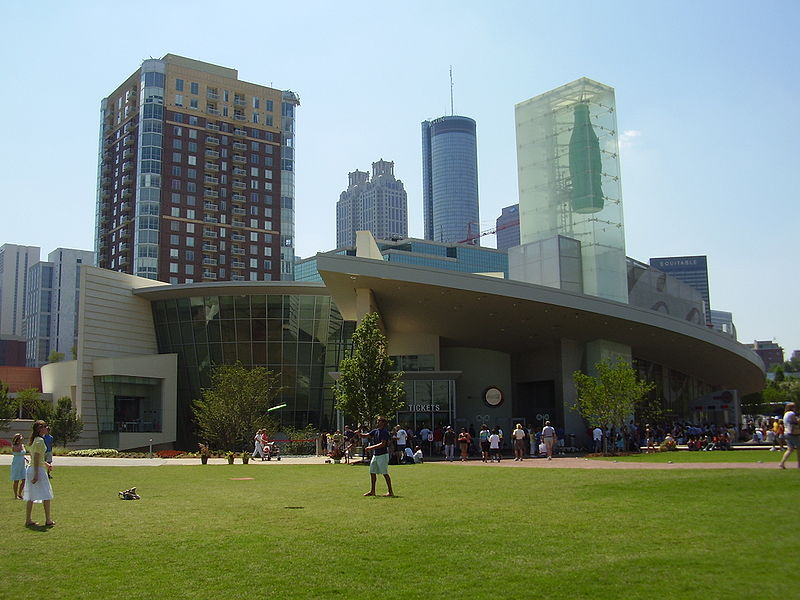
\includegraphics[height=100px]{content/day3/cocacola.jpg}

Tuesday, June 11, 2013, 7:00pm -- 9:00am \vspace{1em}\\
The World of Coca-Cola\\
121 Baker St. NW\\
Atlanta, GA 30313-1807\\
\end{center}

\noindent
This year's NAACL banquet promises to be a unique and interactive experience! Taking place in the intriguing World of Coca Cola Museum, attendees will have access to a multi-sensory 4D theater, an extraordinary 1880s soda fountain, the smallest bottling line in the world, plus an opportunity to sample nearly 70 different beverages from around the globe. Multiple buffet stations and seating areas will allow banquet-goers to enjoy the food and explore the museum at their leisure. And, of course there will be a DJ for your dancing pleasure. The banquet will take place at the World of Coca Cola Museum , Tuesday evening, June 11th. So, save yourselves the standard \$15-16 entrance fee and join us on Tuesday.


\newpage


\clearpage
%\section{Oral Presentations}
\noindent
\vspace{1em}\par\centerline{\bfseries\Large Paper Abstracts}\vspace{1em}\par
\addcontentsline{toc}{section}{Paper Abstracts}
\paperabstract{Tuesday}{10:45am--11:00am}{\Btitle}{\PBC}{main-047}
\paperabstract{Tuesday}{11:00am--11:15am}{\Btitle}{\PBC}{main-022}
\paperabstract{Tuesday}{11:15am--11:30am}{\Btitle}{\PBC}{main-444}
\paperabstract{Tuesday}{11:30am--11:45am}{\Btitle}{\PBC}{main-392}
\paperabstract{Tuesday}{11:45am--12:00pm}{\Btitle}{\PBC}{main-071}
\paperabstract{Tuesday}{10:45am--11:00am}{\Btitle}{\PLZBLRM}{main-016}
\paperabstract{Tuesday}{11:00am--11:15am}{\Btitle}{\PLZBLRM}{main-106}
\paperabstract{Tuesday}{11:15am--11:30am}{\Btitle}{\PLZBLRM}{main-400}
\paperabstract{Tuesday}{11:30am--11:45am}{\Btitle}{\PLZBLRM}{main-310}
\paperabstract{Tuesday}{11:45am--12:00pm}{\Btitle}{\PLZBLRM}{main-314}
\paperabstract{Tuesday}{10:45am--11:00am}{\Btitle}{\PDE}{main-329}
\paperabstract{Tuesday}{11:00am--11:15am}{\Btitle}{\PDE}{main-404}
\paperabstract{Tuesday}{11:15am--11:30am}{\Btitle}{\PDE}{main-455}
\paperabstract{Tuesday}{11:30am--11:45am}{\Btitle}{\PDE}{main-442}
\paperabstract{Tuesday}{11:45am--12:00pm}{\Btitle}{\PDE}{main-353}

\paperabstract{Tuesday}{2:00pm--2:15pm}{\Btitle}{\PBC}{main-001}
\paperabstract{Tuesday}{2:15pm--2:30pm}{\Btitle}{\PBC}{main-119}
\paperabstract{Tuesday}{2:30pm--2:45pm}{\Btitle}{\PBC}{main-037}
\paperabstract{Tuesday}{2:45pm--3:00pm}{\Btitle}{\PBC}{main-197}
\paperabstract{Tuesday}{3:00pm--3:15pm}{\Btitle}{\PBC}{main-434}
\paperabstract{Tuesday}{2:00pm--2:15pm}{\Btitle}{\PLZBLRM}{main-114}
\paperabstract{Tuesday}{2:15pm--2:30pm}{\Btitle}{\PLZBLRM}{main-046}
\paperabstract{Tuesday}{2:30pm--2:45pm}{\Btitle}{\PLZBLRM}{main-163}
\paperabstract{Tuesday}{2:45pm--3:00pm}{\Btitle}{\PLZBLRM}{main-417}
\paperabstract{Tuesday}{3:00pm--3:15pm}{\Btitle}{\PLZBLRM}{main-375}
\paperabstract{Tuesday}{2:00pm--2:15pm}{\Btitle}{\PDE}{main-292}
\paperabstract{Tuesday}{2:15pm--2:30pm}{\Btitle}{\PDE}{main-462}
\paperabstract{Tuesday}{2:30pm--2:45pm}{\Btitle}{\PDE}{main-098}
\paperabstract{Tuesday}{2:45pm--3:00pm}{\Btitle}{\PDE}{main-274}
\paperabstract{Tuesday}{3:00pm--3:15pm}{\Btitle}{\PDE}{main-160}

\clearpage{\thispagestyle{emptyheader}\cleardoublepage}

 
% \chapter{Wednesday, June 12, 2013: Main Conference}
\thispagestyle{emptyheader}
\setheaders{NAACL HLT Main Conference}{Wednesday, June 12, 2013}
\centerline{\bfseries\Large Overview}
\renewcommand{\arraystretch}{1.2}
\begin{SingleTrackSchedule}
 7:00am & -- & 6:00pm &
 {\bfseries Registration} \hfill (\RegLoc)
 \\

 7:30am & -- & 9:00am &
 {\bfseries Continental Breakfast} \hfill (\BreakfastLoc)
 \\

  9:00am & -- & 10:10am & 
  {\bfseries Invited Talk: Kathleen McKeown} \hfill (\ATLBRM)
  \\[1ex]%\hline[-2ex]

  10:10am & -- & 10:40am & {\bfseries Break} \hfill (\BreakLoc)
  \\[1ex]%\hline[-2ex]

  10:40am & -- & 12:20pm & 
  {\bfseries Parallel Sessions}\newline
  \hfill \emph{Machine Translation} \hfill (\MOaLoc)\newline
  \hfill \emph{Semantics} \hfill (\MObLoc)\newline
  \hfill \emph{Social Media Processing} \hfill (\MOcLoc)
  \\[1ex]%\hline[-2ex]
  
  12:20pm & -- & 2:00pm & 
  \bfseries Lunch
  \\[1ex]%\hline[-2ex]

  2:00pm & -- & 3:15pm & 
  {\bfseries Parallel Sessions}\newline
  \hfill \emph{Parsing and Syntax} \hfill (\MOaLoc)\newline
  \hfill \emph{Dialog} \hfill (\MObLoc)\newline
  \hfill \emph{Annotation and Language Resources} \hfill (\MOcLoc)
  \\[1ex]%\hline[-2ex]

  3:15pm & -- & 3:45pm & 
     {\bfseries Break} \hfill (\BreakLoc)
  \\[1ex]%\hline[-2ex]

  3:45pm & -- & 5:00pm & 
  {\bfseries Parallel Sessions}\newline
  \hfill \emph{Semantics and Syntax} \hfill (\MOaLoc)\newline
  \hfill \emph{Summarization and Generation} \hfill (\MObLoc)\newline
  \hfill \emph{Morphology and Phonology} \hfill (\MOcLoc)
  \\[1ex]%\hline[-2ex]

  5:00pm & & & 
  \bfseries Conference adjourns!
  \\[1ex]%\hline[-2ex]

\end{SingleTrackSchedule}

\newpage
%\begin{landscape}
\centerline{\bfseries\Large Schedule}%\vspace{2ex}

\noindent
\begin{ThreeTrackSchedule}
\hline\BreakTime{7:30am}{5:00pm}{3}{Registration (\FOY)}\\\hline\noalign{\bigskip}
%\multicolumn{6}{c}{\ }\\[.25ex]
\hline
\BreakTime   {7:30am}{9:00am}{3}{Breakfast (\FOY)}\\\hline
\PlenaryEvent{9:00am}{10:15am}{3}{{\bfseries Invited Talk (\PLN)}\linebreak
{\itshape J. W. Pennebaker:} {``A, is, I, and, the: How our smallest words reveal the most about who we Are''}\linebreak{\small {\bfseries Chair:} by {\itshape Srinivas Bangalore}}}\\\hline
\BreakTime{10:15am}{10:40am}{3}{Coffee Break (\FOY)}\\\hline

\multicolumn{3}{|c|}{\bfseries Parallel Sessions}
& \bfseries East Ballroom
& \bfseries Center Ballroom
& \bfseries West Ballroom
\\\hline

\multicolumn{3}{|c|}{\bfseries Short Papers}
& \bfseries \SSM 
& \bfseries \SM  
& \bfseries \SU  
\\
&&
& {\small {\bfseries Chair:} {\itshape Theresa Wilson}} 
& {\small {\bfseries Chair:} {\itshape Phil Resnik}} 
& {\small {\bfseries Chair:} {\itshape Ani Nenkova}} 
\\\hline

\input{auto/main/wednesday-main-1}

\end{ThreeTrackSchedule}

\clearpage

\begin{ThreeTrackSchedule}

\hline
\BreakTime{12:00pm}{1:00pm}{3}{Lunch Break}\\\hline

\PlenaryEvent{1:00pm}{2:00pm}{3}{%
{\bfseries NAACL Business Meeting (open to all; \CBR)}}\\\hline

\multicolumn{3}{|c|}{\bfseries Parallel Sessions}
& \bfseries East Ballroom
& \bfseries Center Ballroom
& \bfseries West Ballroom
\\\hline

%\bfseries 2:30pm & -- & \bfseries 4:00pm
&&
& \bfseries \SSM  
& \bfseries \ML~II 
& \bfseries \DDP~II \\
&&
& {\small {\bfseries Chair:} {\itshape Saif Mohammed}} 
& {\small {\bfseries Chair:} {\itshape Scott Yih}} 
& {\small {\bfseries Chair:} {\itshape Diane Litman}} 
\\\hline

\input{auto/main/wednesday-main-2}

\BreakTime{3:40pm}{4:10pm}{3}{Coffee Break (\FOY)}\\\hline

\multicolumn{3}{|c|}{\bfseries Parallel Sessions}
& \bfseries East Ballroom
& \bfseries Center Ballroom
& \bfseries West Ballroom
\\\hline

%\bfseries 2:30pm & -- & \bfseries 4:00pm
&&
& \bfseries \SU  
& \bfseries \SM~II 
& \bfseries \CTM \\
&&
& {\small {\bfseries Chair:} {\itshape Advaith Siddharthan}} 
& {\small {\bfseries Chair:} {\itshape Mona Diab}} 
& {\small {\bfseries Chair:} {\itshape Ryan McDonald}}
\\\hline
\input{auto/main/wednesday-main-3}
\end{ThreeTrackSchedule}
\end{landscape}

%\thispagestyle{myheadings}
\section{Invited Talk: Kathleen McKeown}
\index{McKeown, Kathleen}
\begin{center}
%% --- Keynote Address ---
%% \vspace{2em}\\
%% \vfill

\begin{Large}
{\bfseries\Large ``Natural Language Applications from Fact to Fiction''}\vspace{1em}\par
\end{Large}

{\itshape Kathleen McKeown}\vspace{1em}\par
Wednesday, June 12, 2013, 9:00am -- 10:10am \vspace{1em}\\
\PlenaryLoc
\end{center}

\noindent
{\bfseries Abstract:} Much research in the natural language field has been carried out on news, given the large amount of annotated data now available for this genre.

Certainly, the ability to analyze the facts of real world events, enabling systems to answer questions and summarize the events of the day is an important application. As research has moved to analysis of new genres, whether fact, opinion or fiction, new approaches to existing applications have arisen and opportunities for new applications have emerged. In this talk, I will present research in my group at Columbia as it has moved from news to scientific articles to online discussion forums to novels. I will touch on summarization, open-ended question answering, social influence and social networks.

\vspace{3em}\par 

\vfill
\noindent
{\bfseries Biography:} A leading scholar and researcher in the field of natural language processing,
McKeown focuses her research on big data; her interests include text summarization, question
answering, natural language generation, multimedia explanation, digital libraries, and multilingual
applications. Her research group's Columbia Newsblaster, which has been live since 2001, is an
online system that automatically tracks the day's news, and demonstrates the group's new
technologies for multi-document summarization, clustering, and text categorization, among
others. Currently, she leads a large research project involving prediction of technology emergence
from a large collection of journal articles.

McKeown joined Columbia in 1982, immediately after earning her Ph.D. from University of Pennsylvania. In 1989, she became the first woman professor in the school to receive tenure, and later the first woman to serve as a department chair (1998-2003). McKeown has received numerous honors and awards for her research and teaching. She received the National Science Foundation Presidential Young Investigator Award in 1985, and also is the recipient of a National Science Foundation Faculty Award for Women, was selected as an AAAI Fellow, a Founding Fellow of the Association for Computational Linguistics and an ACM Fellow. In 2010, she won both the Columbia Great Teacher Award—an honor bestowed by the students—and the Anita Borg Woman of Vision Award for Innovation.

McKeown served as a board member of the Computing Research Association and as secretary of the board. She was president of the Association of Computational Linguistics in 1992, vice president in 1991, and secretary treasurer for 1995-1997. She was also a member of the Executive Council of the Association for Artificial Intelligence and the co-program chair of their annual conference in 1991.

\newpage

\newpage

%\section{Oral Presentations}
\vspace{1em}\par\centerline{\bfseries\Large Paper Abstracts}\vspace{1em}\par
\addcontentsline{toc}{section}{Paper Abstracts}
\input{auto/main/wednesday-main-1-B-abstracts.tex}
\input{auto/main/wednesday-main-2-B-abstracts.tex}
\input{auto/main/wednesday-main-3-B-abstracts.tex}
\clearpage{\thispagestyle{emptyheader}\cleardoublepage}

 
% \input{content/star-sem/star-sem}
\vspace*{-3cm}\par
\chapter{Workshops}
\thispagestyle{emptyheader}
\setheaders{Workshops}{June 13--14, 2013}
\section{Overview}
\begin{center}
\renewcommand{\arraystretch}{1.1}
\vspace{-1em}
\begin{tabular}{@{}%
  >{\raggedright\arraybackslash}p{.2\textwidth}
  >{\raggedright\arraybackslash}p{.65\textwidth}
  >{\raggedleft\arraybackslash}p{.05\textwidth}}

  \textbf{Room} & \textbf{Name} & \textbf{Page} \\
\WShopLocA & The 8th Workshop on Innovative Use of NLP for Building Educational Applications (BEA8) &
p.~\pageref{WShopA} \\
\WShopLocB & Seventh Workshop on Syntax, Semantics and Structure in Statistical Translation (SSST-7) & p.~\pageref{WShopB}\\[2em]
\WShopLocC & First workshop on Metaphor in NLP (Meta4NLP) & p.~\pageref{WShopC}\\
\WShopLocD & 9th Workshop on Multiword Expressions (MWE) & p.~\pageref{WShopD}\\
\WShopLocE & Language Analysis in Social Media (LASM) & p.~\pageref{WShopE}\\[3em]
\WShopLocF & Events: Definition, Detection, Coreference, and Representation & p.~\pageref{WShopF}\\
\WShopLocG & Workshop on Vision and Natural Language Processing & p.~\pageref{WShopG}\\
\WShopLocH & Computational Linguistics for Literature & p.~\pageref{WShopH}\\
\WShopLocI & Natural Language Processing for Improving Textual Accessibility (NLP4ITA) & p.~\pageref{WShopI}\\
\WShopLocJ & 4th Workshop on Computational Approaches to Subjectivity, Sentiment and Social Media Analysis (WASSA 2013) & p.~\pageref{WShopJ}\\
\end{tabular}
\end{center}

\clearpage
\setheaders{Workshops}{Thursday, June 13, 2013}
\begin{wsschedule}
{The 8th Workshop on Innovative Use of NLP for Building Educational Applications (BEA8)}
{5}{WShopA}
{The 8th Workshop on Innovative Use of NLP for Building Educational Applications (BEA8)}
{Thursday, June 13}{\WShopLocA}

\item[] {\Large\bfseries Thursday, June 13, 2013
}\\\vspace{1.5ex}

\vspace{1ex}
\item[8:45--9:00] {\bfseries  Load Presentations
}

\vspace{1ex}
\item[9:00--9:15] {\bfseries  Opening Remarks
}

\vspace{1ex}
\item[] {\bfseries Session 1
}
\item[9:15--9:40] \wspaperentry{BEA8-010}
\item[9:40--10:05] \wspaperentry{BEA8-023}
\item[10:05--10:30] \wspaperentry{BEA8-021}

\vspace{1ex}
\item[10:30--11:00] {\bfseries  Break
}

\vspace{1ex}
\item[] {\bfseries Session 2
}
\item[11:00--11:25] \wspaperentry{BEA8-017}
\item[11:25--11:45] \wspaperentry{BEA8-003}
\item[11:45--12:10] \wspaperentry{BEA8-051}

\vspace{1ex}
\item[12:10--1:50] {\bfseries  Lunch
}

\vspace{1ex}
\item[1:50--2:40] {\bfseries  BEA8 Poster Session A
}
\item[$\bullet$] \wspaperentry{BEA8-020}
\item[$\bullet$] \wspaperentry{BEA8-002}
\item[$\bullet$] \wspaperentry{BEA8-007}

\vspace{1ex}
\item[1:50--2:40] {\bfseries  NLI 2013 Poster Session A
}
\item[$\bullet$] \wspaperentry{BEA8-049}
\item[$\bullet$] \wspaperentry{BEA8-039}
\item[$\bullet$] \wspaperentry{BEA8-047}
\item[$\bullet$] \wspaperentry{BEA8-050}
\item[$\bullet$] \wspaperentry{BEA8-031}
\item[$\bullet$] \wspaperentry{BEA8-048}
\item[$\bullet$] \wspaperentry{BEA8-029}
\item[$\bullet$] \wspaperentry{BEA8-045}
\item[$\bullet$] \wspaperentry{BEA8-042}
\item[$\bullet$] \wspaperentry{BEA8-046}
\item[$\bullet$] \wspaperentry{BEA8-044}

\vspace{1ex}
\item[2:40--3:30] {\bfseries  BEA8 Poster Session B
}
\item[$\bullet$] \wspaperentry{BEA8-005}
\item[$\bullet$] \wspaperentry{BEA8-009}
\item[$\bullet$] \wspaperentry{BEA8-016}

\vspace{1ex}
\item[2:40--3:30] {\bfseries  NLI 2013 Poster Session B
}
\item[$\bullet$] \wspaperentry{BEA8-037}
\item[$\bullet$] \wspaperentry{BEA8-032}
\item[$\bullet$] \wspaperentry{BEA8-040}
\item[$\bullet$] \wspaperentry{BEA8-034}
\item[$\bullet$] \wspaperentry{BEA8-027}
\item[$\bullet$] \wspaperentry{BEA8-041}
\item[$\bullet$] \wspaperentry{BEA8-036}
\item[$\bullet$] \wspaperentry{BEA8-033}
\item[$\bullet$] \wspaperentry{BEA8-028}
\item[$\bullet$] \wspaperentry{BEA8-035}
\item[$\bullet$] \wspaperentry{BEA8-038}
\item[$\bullet$] \wspaperentry{BEA8-030}
\item[$\bullet$] \wspaperentry{BEA8-043}

\vspace{1ex}
\item[3:30--4:00] {\bfseries  Break
}

\vspace{1ex}
\item[] {\bfseries Session 3
}
\item[4:00--4:20] \wspaperentry{BEA8-019}
\item[4:20--4:40] \wspaperentry{BEA8-014}
\item[4:40--5:00] \wspaperentry{BEA8-011}
\item[5:00--5:20] \wspaperentry{BEA8-012}

\vspace{1ex}
\item[5:20--5:30] {\bfseries  Closing Remarks
}

\end{wsschedule}
\clearpage
\begin{wsschedule}
{Future directions and needs in the Spoken Dialog Community}
{5}{WShopE}
{Future directions and needs\linebreak in the Spoken Dialog Community}
{Thursday, June7}{\WShopLocE}
\input{content/workshops/sdctd-schedule}
\end{wsschedule}
\clearpage
\begin{wsschedule}
{First workshop on Metaphor in NLP (Meta4NLP)}
{3}{WShopC}
{First workshop on Metaphor in NLP}
{Thursday, June 13}{\WShopLocC}

%\item[] {\Large\bfseries Thursday, June 13, 2013}\\\vspace{1.5ex}

\vspace*{-25px}\par
\item[9:00--9:10] {\bfseries  Opening remarks}

\vspace{1ex}
\item[9:10--10:05] {\bfseries  Invited talk: Srini Narayanan ``From Metaphor to Action''}

\vspace{1ex}
\item[] {\bfseries Session 1}
\item[10:05--10:30] \wspaperentry{Meta4NLP2013-002}

\vspace{1ex}
\item[10:30--11:00] {\bfseries  Coffee break}

\vspace{1ex}
\item[] {\bfseries Session 2}
\item[11:00--11:25] \wspaperentry{Meta4NLP2013-003}
\item[11:25--11:45] \wspaperentry{Meta4NLP2013-012}
\item[11:45--12:10] \wspaperentry{Meta4NLP2013-007}

\vspace{1ex}
\item[12:10--13:40] {\bfseries  Lunch}

\vspace{1ex}
\item[13:40--14:20] {\bfseries  Invited talk: John Barnden ``Computational Approaches to Metaphor Interpretation: Some Considerations arising from a Deep Reasoning System''}

\vspace{1ex}
\item[] {\bfseries Session 3}
\item[14:20--14:45] \wspaperentry{Meta4NLP2013-001}
\item[14:45--15:10] \wspaperentry{Meta4NLP2013-009}
\item[15:10--15:30] \wspaperentry{Meta4NLP2013-006}

\vspace{1ex}
\item[15:30--16:00] {\bfseries  Coffee break}

\vspace{1ex}
\item[] {\bfseries Session 4}
\item[16:00--16:25] \wspaperentry{Meta4NLP2013-013}
\item[16:25--16:50] \wspaperentry{Meta4NLP2013-005}
\item[16:50--17:15] \wspaperentry{Meta4NLP2013-014}

\vspace{1ex}
\item[17:15--17:30] {\bfseries  Closing remarks}

\end{wsschedule}
\clearpage
\begin{wsschedule}
{9th workshop on Multiword Expressions (MWE)}
{4}{WShopD}
{9th workshop on Multiword Expressions (MWE)}
{Thursday, June 13}{\WShopLocD}

%\item[] {\Large\bfseries Thursday, June 13, 2013
%}\\\vspace{1.5ex}

\vspace{1ex}
\item[09:00--09:15] {\bfseries  Opening Remarks
}

\vspace{1ex}
\item[] {\bfseries Oral Session 1: Resources and Applications
}
\item[09:15--09:40] \wspaperentry{MWE2013-003}
\item[09:40--10:05] \wspaperentry{MWE2013-017}
\item[10:05--10:30] \wspaperentry{MWE2013-021}

\vspace{1ex}
\item[10:30--11:00] {\bfseries  COFFEE BREAK
}

\vspace{1ex}
\item[] {\bfseries Invited Talk 1
}
\item[11:00--12:00] \wspaperentry{MWE2013-030}

\vspace{1ex}
\item[] {\bfseries Oral Session 2: Compositionality
}
\item[12:00--12:25] \wspaperentry{MWE2013-023}

\vspace{1ex}
\item[12:30-14:00] {\bfseries  LUNCH BREAK
}

\vspace{1ex}
\item[] {\bfseries Oral Session 2: Compositionality (continued)
}
\item[14:05--14:30] \wspaperentry{MWE2013-020}

\vspace{1ex}
\item[] {\bfseries Invited Talk 2
}
\item[14:30--15:30] \wspaperentry{MWE2013-029}

\vspace{1ex}
\item[15:30--16:00] {\bfseries  COFFEE BREAK
}

\vspace{1ex}
\item[] {\bfseries Oral Session 3: Short Papers
}
\item[16:00--16:15] \wspaperentry{MWE2013-009}
\item[16:15--16:30] \wspaperentry{MWE2013-012}

\vspace{1ex}
\item[16:30--16:40] {\bfseries  Poster Boosters
}
\item[$\bullet$] \wspaperentry{MWE2013-007}
\item[$\bullet$] \wspaperentry{MWE2013-011}
\item[$\bullet$] \wspaperentry{MWE2013-013}
\item[$\bullet$] \wspaperentry{MWE2013-019}
\item[$\bullet$] \wspaperentry{MWE2013-022}
\item[$\bullet$] \wspaperentry{MWE2013-026}

\vspace{1ex}
\item[16:30--17:40] {\bfseries  Poster Session
}

\item[] {\Large\bfseries Friday, June 14, 2013
}\\\vspace{1.5ex}

\vspace{1ex}
\item[] {\bfseries Oral Session 4: Identification and Classification
}
\item[09:10--09:35] \wspaperentry{MWE2013-014}
\item[09:35--10:00] \wspaperentry{MWE2013-002}

\vspace{1ex}
\item[] {\bfseries Oral Session 5: Short Papers
}
\item[10:00--10:15] \wspaperentry{MWE2013-004}
\item[10:15--10:30] \wspaperentry{MWE2013-028}

\vspace{1ex}
\item[10:30--11:00] {\bfseries  COFFEE BREAK
}

\vspace{1ex}
\item[] {\bfseries Invited Talk 3
}
\item[11:00--12:00] \wspaperentry{MWE2013-031}

\vspace{1ex}
\item[] {\bfseries Oral Session 5: Short Papers (continued)
}
\item[12:00--12:15] \wspaperentry{MWE2013-016}

\vspace{1ex}
\item[12:15--12:30] {\bfseries  Closing Remarks}

\end{wsschedule}
\clearpage
\begin{wsschedule}
{Language Analysis in Social Media (LASM)}
{5}{WShopE}
{Language Analysis in Social Media (LASM)}
{Thursday, June 13}{\WShopLocE}

%\item[] {\Large\bfseries Thursday, June 13, 2013}\\\vspace{1.5ex}

\vspace{1ex}
\item[9:00--9:15] {\bfseries  Introductions}

\vspace{1ex}
\item[9:15--10:30] {\bfseries  Invited Key Note, Prof. Mor Naaman}

\vspace{1ex}
\item[10:30--11:00] {\bfseries  Coffee Break}

\vspace{1ex}
\item[] {\bfseries Session 1}
\item[11:00--11:30] \wspaperentry{LASM2013-001}
\item[11:30--12:00] \wspaperentry{LASM2013-002}
\item[12:00--12:30] \wspaperentry{LASM2013-015}

\vspace{1ex}
\item[12:30--2:00] {\bfseries  Lunch}

\vspace{1ex}
\item[] {\bfseries Session 2}
\item[2:00--2:30] \wspaperentry{LASM2013-010}
\item[2:30--3:00] \wspaperentry{LASM2013-011}
\item[3:00--3:30] \wspaperentry{LASM2013-014}

\vspace{1ex}
\item[3:30--3:45] {\bfseries  Coffee Break}

\vspace{1ex}
\item[] {\bfseries Session 3}
\item[3:45--4:15] \wspaperentry{LASM2013-006}
\item[4:15--4:45] \wspaperentry{LASM2013-017}
\item[4:45--5:15] \wspaperentry{LASM2013-007}

\vspace{1ex}
\item[5:15--5:30] {\bfseries  Closing Remarks}

\end{wsschedule}
\clearpage
\setheaders{Workshops}{Friday, June 14, 2013}
\begin{wsschedule}
{Events: Definition, Detection, Coreference, and Representation (EVENTS)}
{5}{WShopF}
{Events: Definition, Detection, Coreference, and Representation (EVENTS)}
{Thursday, June13}{\WShopLocF}

%\item[] {\Large\bfseries Friday, June 14, 2013}\\\vspace{1.5ex}

\vspace*{-25px}\par
\item[9:00--9:15] {\bfseries  Welcome}

\vspace{1ex}
\item[9:15--9:30] {\bfseries  Working Session Instructions}

\vspace{1ex}
\item[9:30--10:30] {\bfseries  Invited Talk: The Role of Event-based Representations and Reasoning in Language, James Pustejovsky}

\vspace{1ex}
\item[10:30--11:00] {\bfseries  Break}

\vspace{1ex}
\item[11:00--12:00] {\bfseries  Working Session I: What are events?}

\vspace{1ex}
\item[12:00--1:00] {\bfseries  Poster Session}
\item[$\bullet$] \wspaperentry{EVENTS-001}
\item[$\bullet$] \wspaperentry{EVENTS-002}
\item[$\bullet$] \wspaperentry{EVENTS-003}
\item[$\bullet$] \wspaperentry{EVENTS-004}
\item[$\bullet$] \wspaperentry{EVENTS-005}
\item[$\bullet$] \wspaperentry{EVENTS-006}

\vspace{1ex}
\item[2:00--3:30] {\bfseries  Working Session II: When are two events the same? What relations are between events?}

\vspace{1ex}
\item[3:30--4:00] {\bfseries  Break}

\vspace{1ex}
\item[4:00--5:30] {\bfseries  Working Session III: How best to represent events? What aspects to annotate?}

\vspace{1ex}
\item[5:30--6:00] {\bfseries  General Discussion}

\end{wsschedule}
\clearpage
\begin{wsschedule}
{Future directions and needs in the Spoken Dialog Community}
{5}{WShopE}
{Future directions and needs\linebreak in the Spoken Dialog Community}
{Thursday, June7}{\WShopLocE}
\input{content/workshops/sdctd-schedule}
\end{wsschedule}
\clearpage
\begin{wsschedule}
{Computational Linguistics for Literature (CLFL)}
{8}{WShopH}
{Computational Linguistics for Literature (CLFL)}
{Thursday, June 13}{\WShopLocH}

%\item[] {\Large\bfseries Friday, June 14, 2013}\\\vspace{1.5ex}

\vspace{1ex}
\item[9:00--9:05] {\bfseries  Welcome}

\vspace{1ex}
\item[9:05-10:00] {\bfseries  Invited talk by Livia Polanyi}
\item[10:00-10:30] \wspaperentry{CLfL-004}

\vspace{1ex}
\item[10:30-11:00] {\bfseries  Coffee break}
\item[11:00-11:30] \wspaperentry{CLfL-011}
\item[11:30-12:00] \wspaperentry{CLfL-015}
\item[12:00-12:30] \wspaperentry{CLfL-005}

\vspace{1ex}
\item[12:30-14:00] {\bfseries  Lunch break}

\vspace{1ex}
\item[14:00-15:00] {\bfseries  Invited talk by Mark Riedl}

\vspace{1ex}
\item[15:00-15:30] {\bfseries  Poster teasers}
\item[$\bullet$] \wspaperentry{CLfL-009}
\item[$\bullet$] \wspaperentry{CLfL-001}
\item[$\bullet$] \wspaperentry{CLfL-012}
\item[$\bullet$] \wspaperentry{CLfL-007}
\item[$\bullet$] \wspaperentry{CLfL-003}

\vspace{1ex}
\item[15:30-16:00] {\bfseries  Coffee break}

\vspace{1ex}
\item[16:00-16:30] {\bfseries  Poster session}
\item[16:30-17:00] \wspaperentry{CLfL-006}

\vspace{1ex}
\item[17:00-17:30] {\bfseries  An informal talk by He, Barbosa and Kondrak}

\vspace{1ex}
\item[17:30--18:00] {\bfseries  Farewell}

\end{wsschedule}
\clearpage
\begin{wsschedule}
{Natural Language Processing for Improving Textual Accessibility (NLP4ITA)}
{5}{WShopI}
{Natural Language Processing for Improving Textual Accessibility (NLP4ITA)}
{Thursday, June 13}{\WShopLocI}

%\item[] {\Large\bfseries Friday, June 14, 2013}\\\vspace{1.5ex}

\vspace*{-25px}\par
\item[9:15--9:30] {\bfseries  Opening Remarks by Workshop Chairs}
\item[9:30--10:00] \wspaperentry{NLP4ITA2013-002}
\item[10:00--10:30] \wspaperentry{NLP4ITA2013-010}

\vspace{1ex}
\item[10:30--11:00] {\bfseries  Coffee Break}
\item[11:00--11:30] \wspaperentry{NLP4ITA2013-006}

\vspace{1ex}
\item[11:30--12:30] {\bfseries  Invited Talk: {\em Information Accessibility: More than just text
deep} (Kathleen F. McCoy, University of Delaware, USA)}

\vspace{1ex}
\item[12:30--14:00] {\bfseries  Lunch Break}
\item[14:00--14:30] \wspaperentry{NLP4ITA2013-005}
\item[14:30--15:00] \wspaperentry{NLP4ITA2013-003}
\item[15:00--15:30] \wspaperentry{NLP4ITA2013-007}

\vspace{1ex}
\item[15:30--16:00] {\bfseries  Coffee Break}

\vspace{1ex}
\item[16:00--17:00] {\bfseries  Final Discussion and Closing Remarks}

\end{wsschedule}
\clearpage
\begin{wsschedule}
{Future directions and needs in the Spoken Dialog Community}
{5}{WShopE}
{Future directions and needs\linebreak in the Spoken Dialog Community}
{Thursday, June7}{\WShopLocE}
\input{content/workshops/sdctd-schedule}
\end{wsschedule}
\clearpage
\clearpage{\thispagestyle{emptyheader}\cleardoublepage}


\clearpage
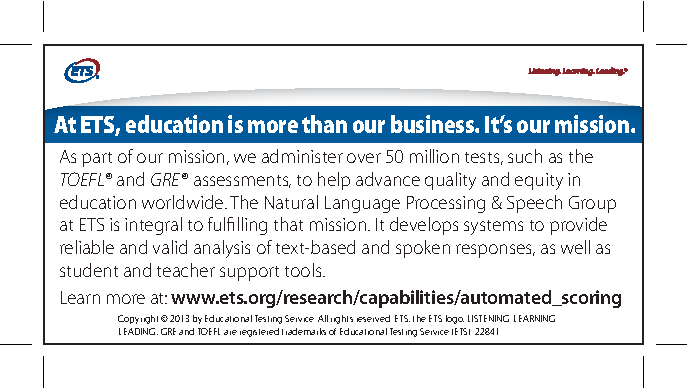
\includegraphics{ads/ETS.pdf}
\vfill{30px}

\includegraphics[height=300px]{ads/ISI.pdf}


\cleardoublepage
\setheaders{Author Index}{Author Index}
\printindex


\includegraphics[height=300px]{ads/SDL_Research_Hire_Ad_4x4_Color.jpg}
\vfill{30px}

\includegraphics{ads/AppenButlerHill-gif.jpg}


\setheaders{Hotel Maps}{Hotel Maps}
\chapter{Maps}
\thispagestyle{emptyheader}
\setheaders{Maps}{Maps}
\vspace{-3em}
\sloppy
%\addcontentsline{toc}{chapter}{Sunday, Jun 9, 2013: Tutorials}
\setlength{\parindent}{0in}
\setlength{\parskip}{2ex}
\renewcommand{\baselinestretch}{0.87}

\begin{center}
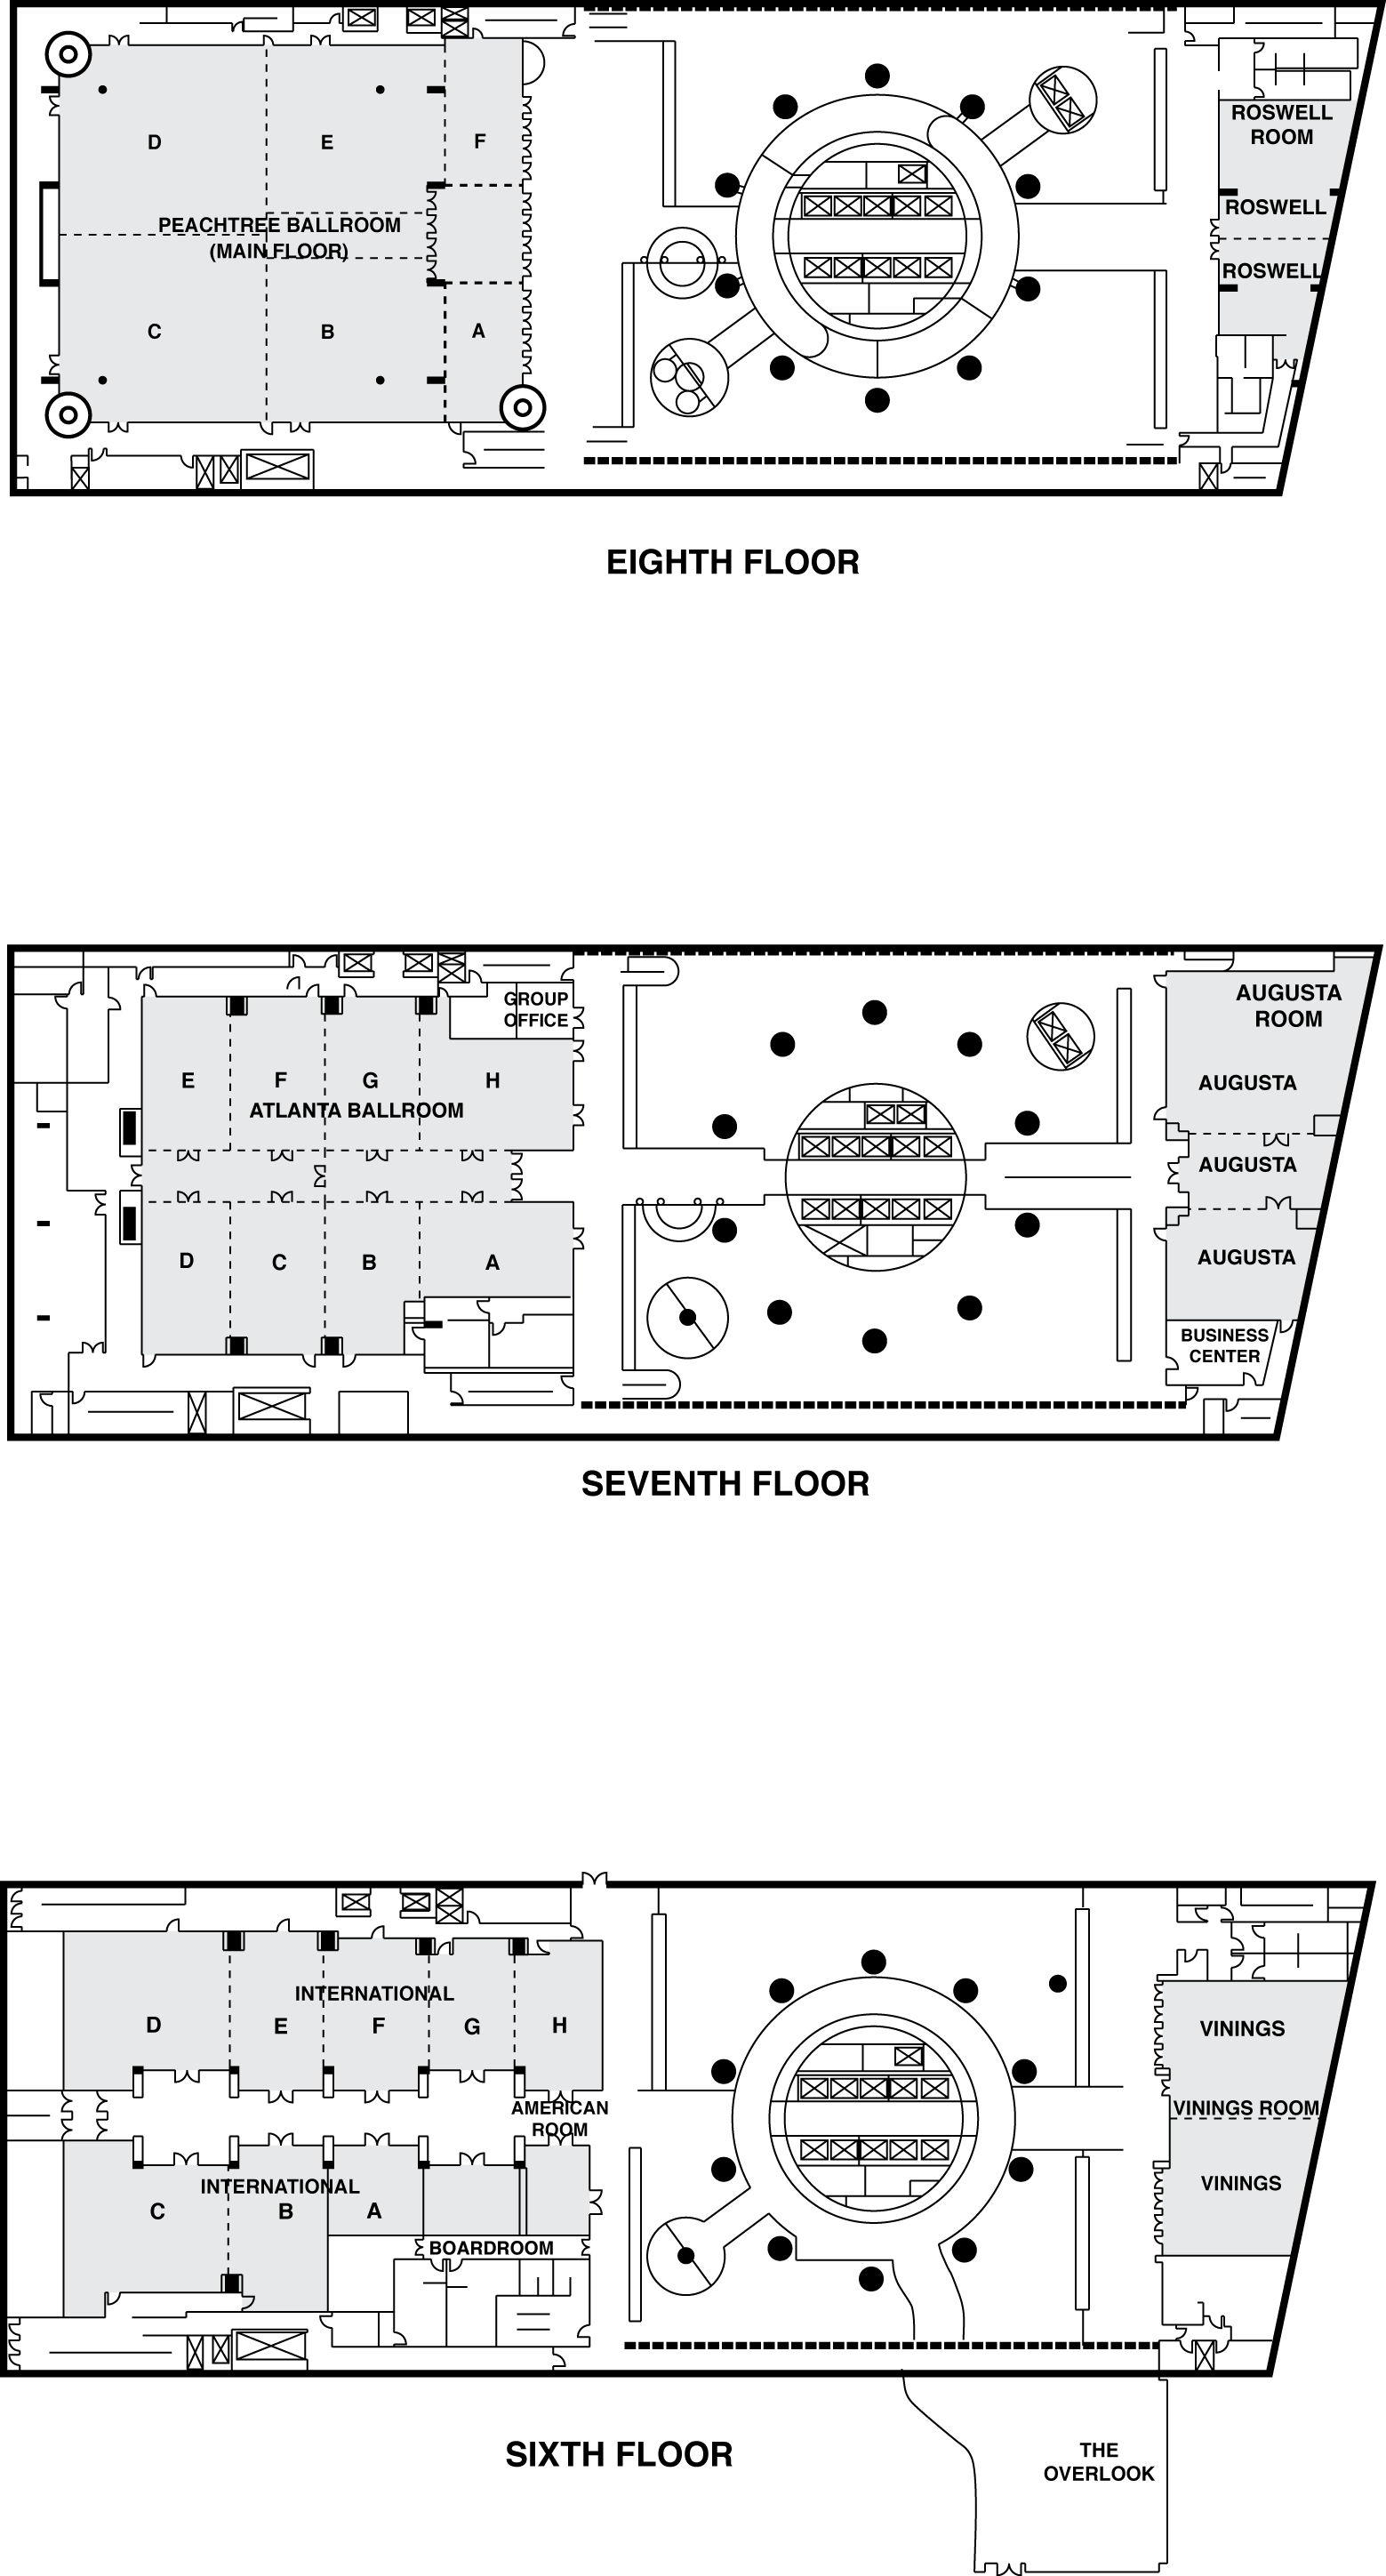
\includegraphics[height=450px]{content/map1.png}
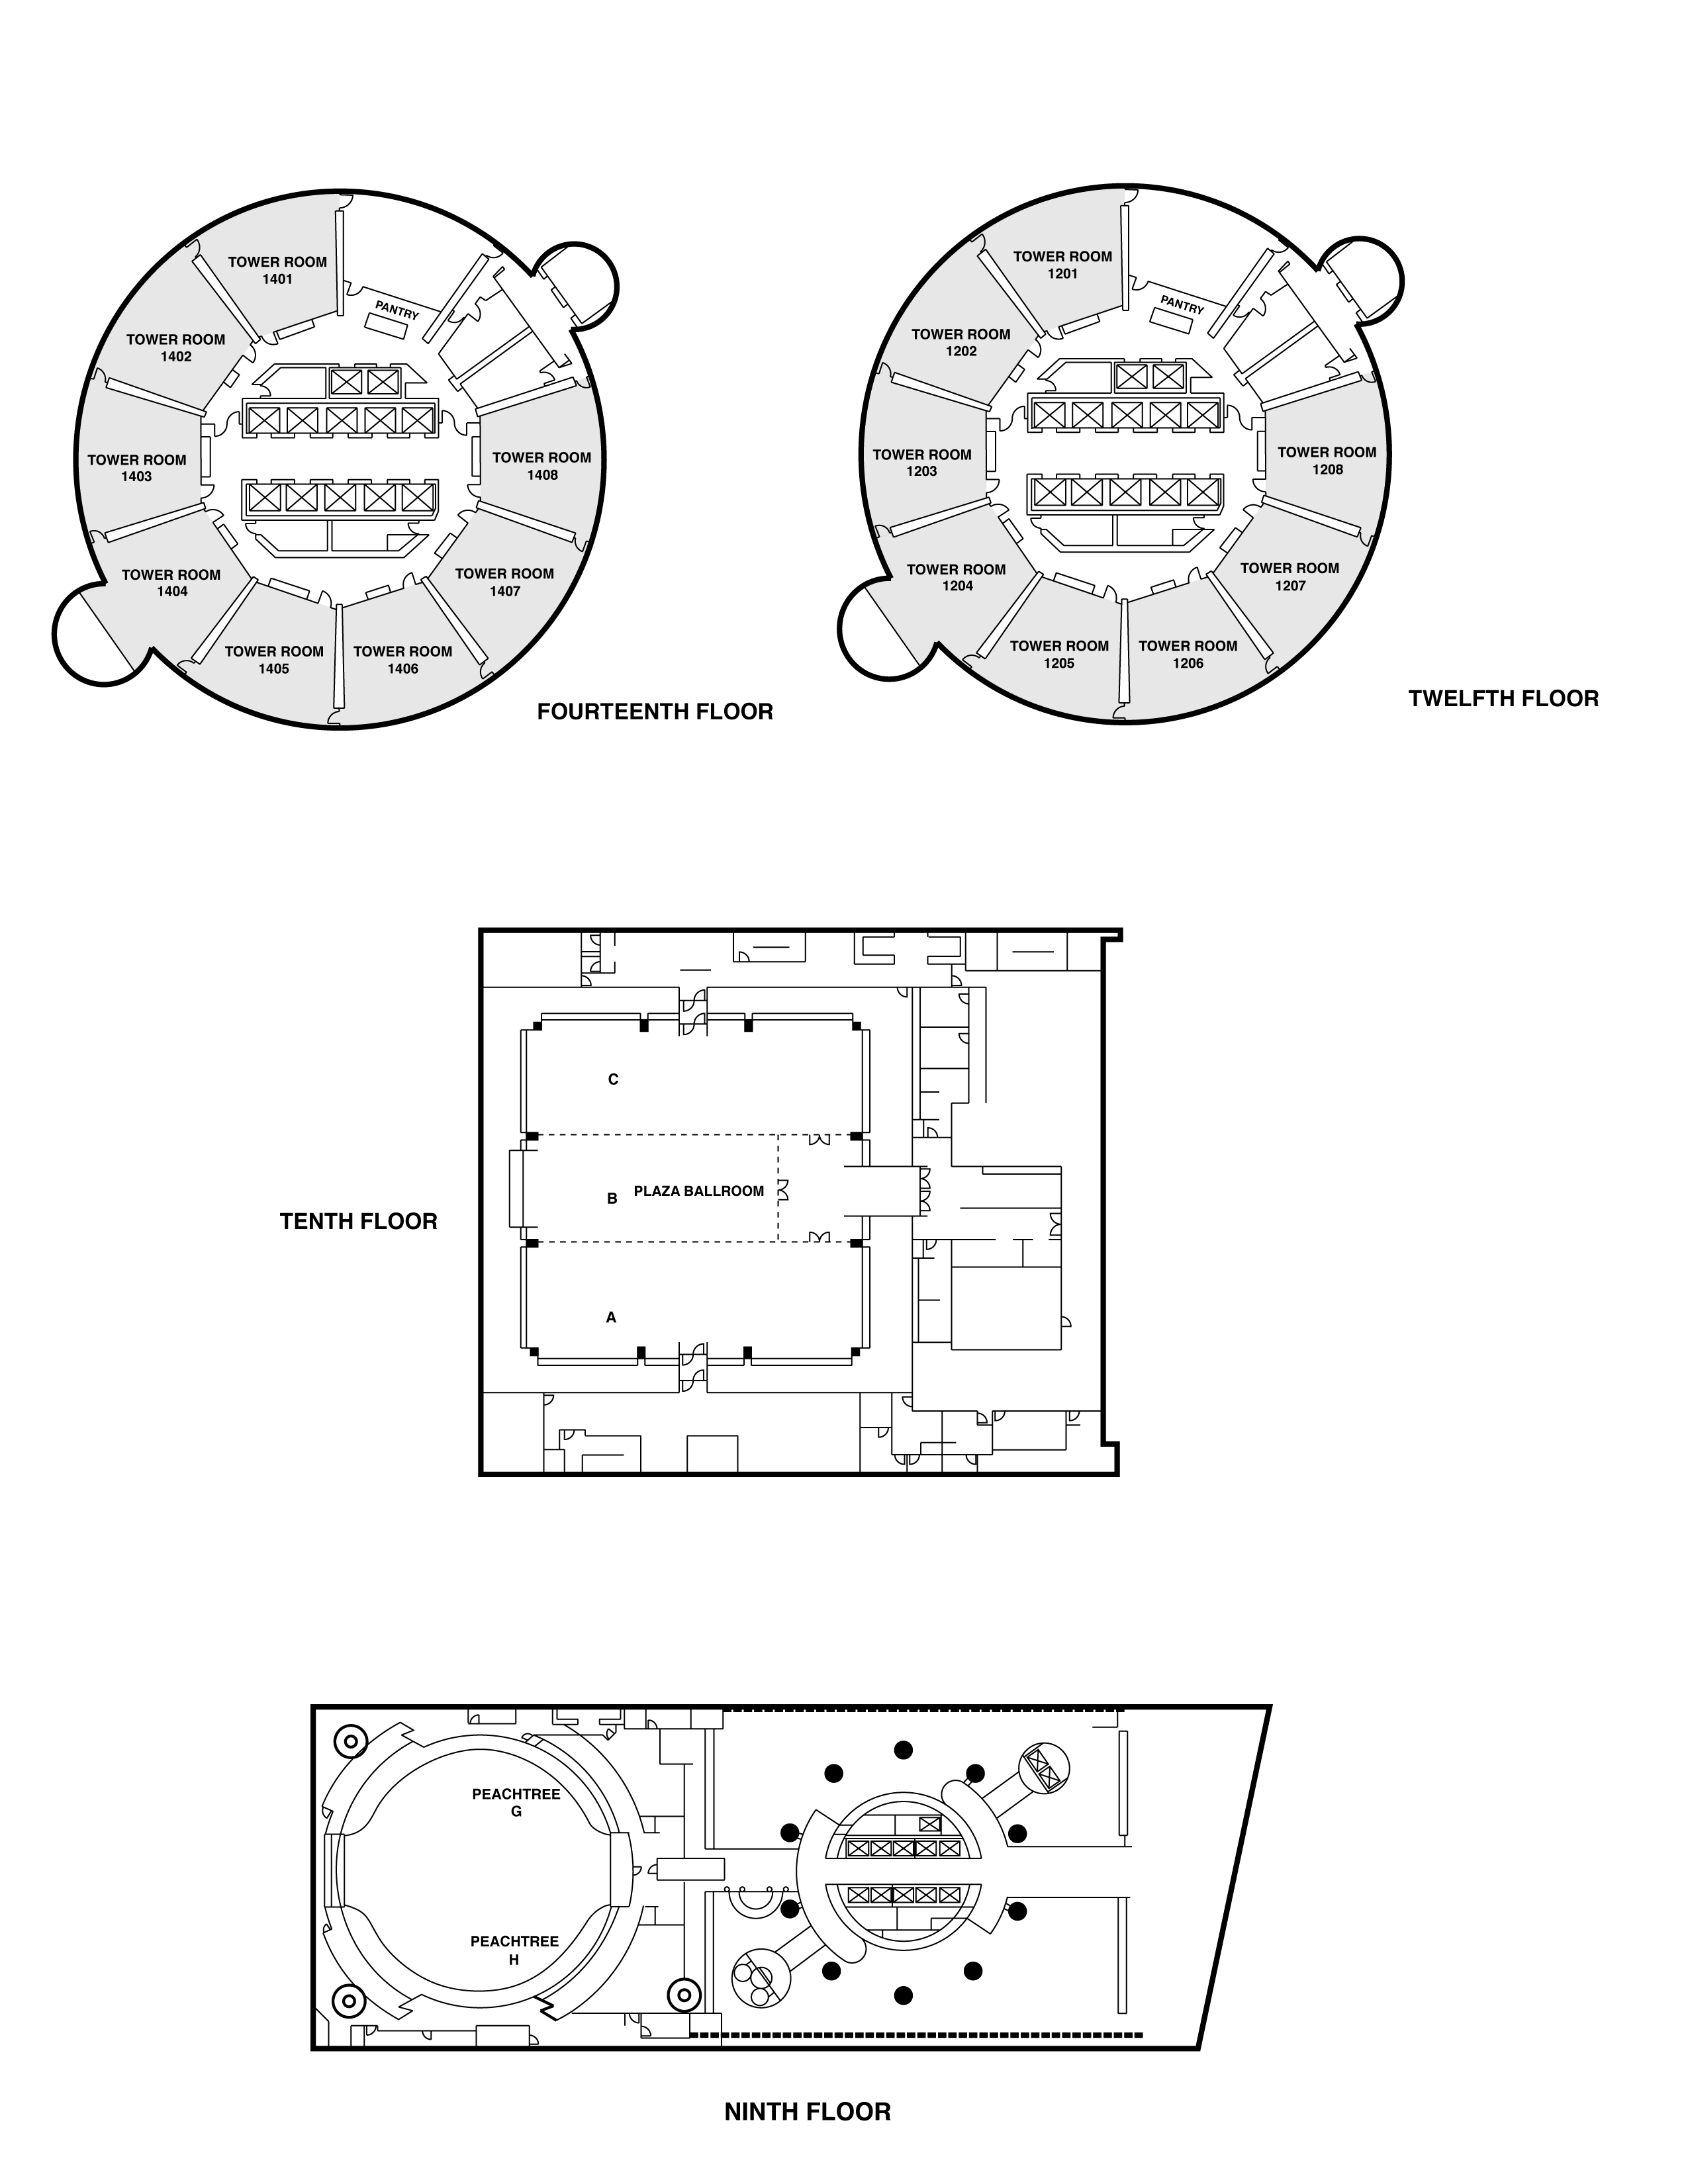
\includegraphics[height=420px]{content/map2.png}
\end{center}


\thispagestyle{empty}

%% \vfill
\large\emph{NAACL HLT 2013 gratefully acknowledges the following sponsors for their support.}

\vspace*{0.5cm}

%
% SPONSOR LOGOS
%
{\bf \large Gold Level}\vspace{5mm} \\
\begin{tabular*}{\textwidth}{@{\extracolsep{\fill}} lll }
    
\includegraphics[width=1.4in]{content/fmatter/sponsors/google.pdf} 
    & 
\includegraphics[width=1.4in]{content/fmatter/sponsors/microsoft_research.pdf} \\
\end{tabular*} \\

\vspace{10mm}
{\bf \large Bronze Level}\vspace{5mm} \\
\begin{tabular*}{\textwidth}{@{\extracolsep{\fill}} lll }
  
\includegraphics[width=1.4in]{content/fmatter/sponsors/ets.pdf}
  & 
\includegraphics[width=1.4in]{content/fmatter/sponsors/rakuten-logo.pdf}
  & 
\includegraphics[width=1.4in]{content/fmatter/sponsors/abh-logo.pdf} \\
\end{tabular*} \\

\vspace{10mm}
{\bf \large Student Best Paper Award and Student Lunch Sponsor}\vspace{5mm} \\
\hspace*{5mm}
\includegraphics[width=1.4in]{content/fmatter/sponsors/IBM_Research.pdf} \\

\vspace{10mm}
{\bf \large Student Volunteer Sponsor}\vspace{5mm} \\
%\hspace*{5mm}University of Southern California, Information Sciences Institute \\
\hspace*{5mm}
\includegraphics[width=1.4in]{content/fmatter/sponsors/usc-logo.pdf}

\vspace{10mm}
{\bf \large Conference Bags}\vspace*{5mm} \\
\hspace*{5mm}
\includegraphics[width=1.4in]{content/fmatter/sponsors/sdl-logo.pdf}

\vfill

\end{document}
%%%%%%%%%%%%%%%%%%%%%%%%%%%%%%%%%%%%%%%%%%%%%%%%%%
